\section{SQL DDL}

% Define colors that match VSCode Light theme
\definecolor{vscode-background}{HTML}{FFFFFF} % White background
\definecolor{vscode-foreground}{HTML}{000000} % Default black text color
\definecolor{vscode-keyword}{HTML}{0000FF}    % Blue for keywords
\definecolor{vscode-comment}{HTML}{008000}    % Green for comments
\definecolor{vscode-string}{HTML}{A31515}     % Red for strings
\definecolor{vscode-function}{HTML}{795E26}   % Brown for function names
\definecolor{vscode-line-numbers}{HTML}{AAAAAA} % Light gray for line numbers

\lstset{
  language=SQL,
  basicstyle=\ttfamily\small,  % Set font style and size
  numbers=left,                % Line numbers on the left
  numberstyle=\tiny\color{gray},
  keywordstyle=\color{vscode-keyword},    % keywords in blue
  commentstyle=\color{vscode-comment},    % comments in green
  stringstyle=\color{vscode-string},      % strings in red
  stepnumber=1,
  showstringspaces=false,
  breaklines=true,
  frame=single,
  rulecolor=\color{black},
  tabsize=2,
  breakatwhitespace=false,                % don't break at whitespace
  upquote=true,
  captionpos=b,
}

\subsection{Queries}

\subsubsection{Create Queries}

First of all, let us define the domains.
\lstinputlisting[language=SQL, caption={\textit{Create Domains}}]{sql/domains.sql}

\subsubsubsection{Supplier}

The following script creates the Supplier table.
\lstinputlisting[language=SQL, caption={\textit{Create Supplier Table}}]{sql/create/supplier.sql}

\subsubsubsection{Category}

The following script creates the Category table.
\lstinputlisting[language=SQL, caption={\textit{Create Category Table}}]{sql/create/category.sql}

\subsubsubsection{Product}

The following script creates the Product table.
\lstinputlisting[language=SQL, caption={\textit{Create Product Table}}]{sql/create/product.sql}

\subsubsubsection{Branch}

The following script creates the Branch table.
\lstinputlisting[language=SQL, caption={\textit{Create Branch Table}}]{sql/create/branch.sql}

\subsubsubsection{Department}

The following script creates the Department table.
\lstinputlisting[language=SQL, caption={\textit{Create Department Table}}]{sql/create/department.sql}

\subsubsubsection{Employee}

The following script creates the Employee table.
\lstinputlisting[language=SQL, caption={\textit{Create Employee Table}}]{sql/create/employee.sql}

\subsubsubsection{Driver}

The following script creates the Driver table.
\lstinputlisting[language=SQL, caption={\textit{Create Driver Table}}]{sql/create/driver.sql}

\subsubsubsection{Customer}

The following script creates the Customer table.
\lstinputlisting[language=SQL, caption={\textit{Create Customer Table}}]{sql/create/customer.sql}

\subsubsubsection{Order}

The following script creates the Order table.
\lstinputlisting[language=SQL, caption={\textit{Create Order Table}}]{sql/create/orders.sql}

\subsubsubsection{Purchased}

The following script creates the Purchased table.
\lstinputlisting[language=SQL, caption={\textit{Create Purchased Table}}]{sql/create/purchased.sql}

\subsubsubsection{Reviews}

The following script creates the Reviews table.
\lstinputlisting[language=SQL, caption={\textit{Create Reviews Table}}]{sql/create/reviews.sql}

\subsubsubsection{Support Ticket}

The following script creates the Support Ticket table.
\lstinputlisting[language=SQL, caption={\textit{Create Support Ticket Table}}]{sql/create/support_ticket.sql}

\subsubsubsection{Wishlist}

The following script creates the Wishlist table.
\lstinputlisting[language=SQL, caption={\textit{Create Wishlist Table}}]{sql/create/wishlist.sql}

\subsubsubsection{Working hours}

The following script creates the Working hours table.
\lstinputlisting[language=SQL, caption={\textit{Create Working Hours Table}}]{sql/create/working_hours.sql}

\subsubsubsection{Dependent}

The following script creates the Dependent table.
\lstinputlisting[language=SQL, caption={\textit{DCreate ependent Table}}]{sql/create/dependent.sql}

\subsubsubsection{Product Image URLs}

The following script creates the Product Image URLs table.
\lstinputlisting[language=SQL, caption={\textit{Create Product Image URLs Table}}]{sql/create/product_image_urls.sql}

\subsubsubsection{Review Image URLs}

The following script creates the Review Image URLs table.
\lstinputlisting[language=SQL, caption={\textit{Create Review Image URLs Table}}]{sql/create/review_image_urls.sql}

\subsubsubsection{Located in}

The following script creates the Located in table.
\lstinputlisting[language=SQL, caption={\textit{Create Located In Table}}]{sql/create/located_in.sql}

\subsubsubsection{Colors}

The following script creates the Colors table.
\lstinputlisting[language=SQL, caption={\textit{Create Colors Table}}]{sql/create/colors.sql}

\subsubsubsection{Coupon}

The following script creates the Coupon table.
\lstinputlisting[language=SQL, caption={\textit{Create Coupon Table}}]{sql/create/coupon.sql}

\subsubsubsection{Department location}

The following script creates the Department location table.
\lstinputlisting[language=SQL, caption={\textit{Create Department Location Table}}]{sql/create/department_location.sql}

\subsubsection{Alter Queries}

\subsubsubsection{Branch}

The following script alters the Branch table.
\lstinputlisting[language=SQL, caption={\textit{Alter Branch Table}}]{sql/alter/branch.sql}

\subsubsubsection{Department}

The following script alters the Department table.
\lstinputlisting[language=SQL, caption={\textit{Alter Department Table}}]{sql/alter/department.sql}

\subsubsection{Insert Queries}

\subsubsubsection{Supplier}

The following script inserts data into the Supplier table.
\lstinputlisting[language=SQL, caption={\textit{Insert into Supplier Table}}]{sql/insert/supplier.sql}

\subsubsubsection{Category}

The following script inserts data into the Category table.
\lstinputlisting[language=SQL, caption={\textit{Insert into Category Table}}]{sql/insert/category.sql}

\subsubsubsection{Product}

The following script inserts data into the Product table.
\lstinputlisting[language=SQL, caption={\textit{Insert into Product Table}}]{sql/insert/product.sql}

\subsubsubsection{Branch \& Department \& Employee}

\begin{enumerate}[label=Step \arabic*:]
  \item Insert departments with Employee\_SSN as NULL
        \lstinputlisting[language=SQL, caption={\textit{Insert into Department Table}}]{sql/insert/branch-department-employee/1.sql}
  \item Insert branches with Employee\_SSN as NULL
        \lstinputlisting[language=SQL, caption={\textit{Insert into Branch Table}}]{sql/insert/branch-department-employee/2.sql}
  \item Insert employees referencing Department\_name
        \lstinputlisting[language=SQL, caption={\textit{Insert into Employee Table}}]{sql/insert/branch-department-employee/3.sql}
  \item Update departments to set Employee\_SSN (manager's SSN)
        \lstinputlisting[language=SQL, caption={\textit{Update Department Table}}]{sql/insert/branch-department-employee/4.sql}
  \item Update branches to set Employee\_SSN
        \lstinputlisting[language=SQL, caption={\textit{Update Branch Table}}]{sql/insert/branch-department-employee/5.sql}
\end{enumerate}

Finally wrap the whole code with a transaction block. Add \texttt{BEGIN;} at the beginning and \texttt{COMMIT;} at the end.

The final script is as follows:
\lstinputlisting[language=SQL, caption={\textit{Insert into Branch, Department, and Employee Tables}}]{sql/insert/branch-department-employee.sql}

\subsubsubsection{Driver}

The following script inserts data into the Driver table.
\lstinputlisting[language=SQL, caption={\textit{Insert into Driver Table}}]{sql/insert/driver.sql}

\subsubsubsection{Customer}

The following script inserts data into the Customer table.
\lstinputlisting[language=SQL, caption={\textit{Insert into Customer Table}}]{sql/insert/customer.sql}

\subsubsubsection{Order}

The following script inserts data into the Order table.
\lstinputlisting[language=SQL, caption={\textit{Insert into Order Table}}]{sql/insert/orders.sql}

\subsubsubsection{Purchased}

The following script inserts data into the Purchased table.
\lstinputlisting[language=SQL, caption={\textit{Insert into Purchased Table}}]{sql/insert/purchased.sql}

\subsubsubsection{Reviews}

The following script inserts data into the Reviews table.
\lstinputlisting[language=SQL, caption={\textit{Insert into Reviews Table}}]{sql/insert/reviews.sql}

\subsubsubsection{Support Ticket}

The following script inserts data into the Support Ticket table.
\lstinputlisting[language=SQL, caption={\textit{Insert into Support Ticket Table}}]{sql/insert/support_ticket.sql}

\subsubsubsection{Wishlist}

The following script inserts data into the Wishlist table.
\lstinputlisting[language=SQL, caption={\textit{Insert into Wishlist Table}}]{sql/insert/wishlist.sql}

\subsubsubsection{Working hours}

The following script inserts data into the Working hours table.
\lstinputlisting[language=SQL, caption={\textit{Insert into Working Hours Table}}]{sql/insert/working_hours.sql}

\subsubsubsection{Dependent}

The following script inserts data into the Dependent table.
\lstinputlisting[language=SQL, caption={\textit{Insert into Dependent Table}}]{sql/insert/dependent.sql}

\subsubsubsection{Product Image URLs}

The following script inserts data into the Product Image URLs table.
\lstinputlisting[language=SQL, caption={\textit{Insert into Product Image URLs Table}}]{sql/insert/product_image_urls.sql}

\subsubsubsection{Review Image URLs}

The following script inserts data into the Review Image URLs table.
\lstinputlisting[language=SQL, caption={\textit{Insert into Review Image URLs Table}}]{sql/insert/review_image_urls.sql}

\subsubsubsection{Located in}

The following script inserts data into the Located in table.
\lstinputlisting[language=SQL, caption={\textit{Insert into Located In Table}}]{sql/insert/located_in.sql}

\subsubsubsection{Colors}

The following script inserts data into the Colors table.
\lstinputlisting[language=SQL, caption={\textit{Insert into Colors Table}}]{sql/insert/colors.sql}

\subsubsubsection{Coupon}

The following script inserts data into the Coupon table.
\lstinputlisting[language=SQL, caption={\textit{Insert into Coupon Table}}]{sql/insert/coupon.sql}

\subsubsubsection{Department location}

The following script inserts data into the Department location table.
\lstinputlisting[language=SQL, caption={\textit{Insert into Department Location Table}}]{sql/insert/department_location.sql}

\subsubsection{Select Queries}

\subsubsubsection{Supplier}
The following script selects data from the Supplier table.
\lstinputlisting[language=SQL, caption={\textit{Select from Supplier Table}}]{sql/select/supplier.sql}

\begin{figure}[H]
  \centering
  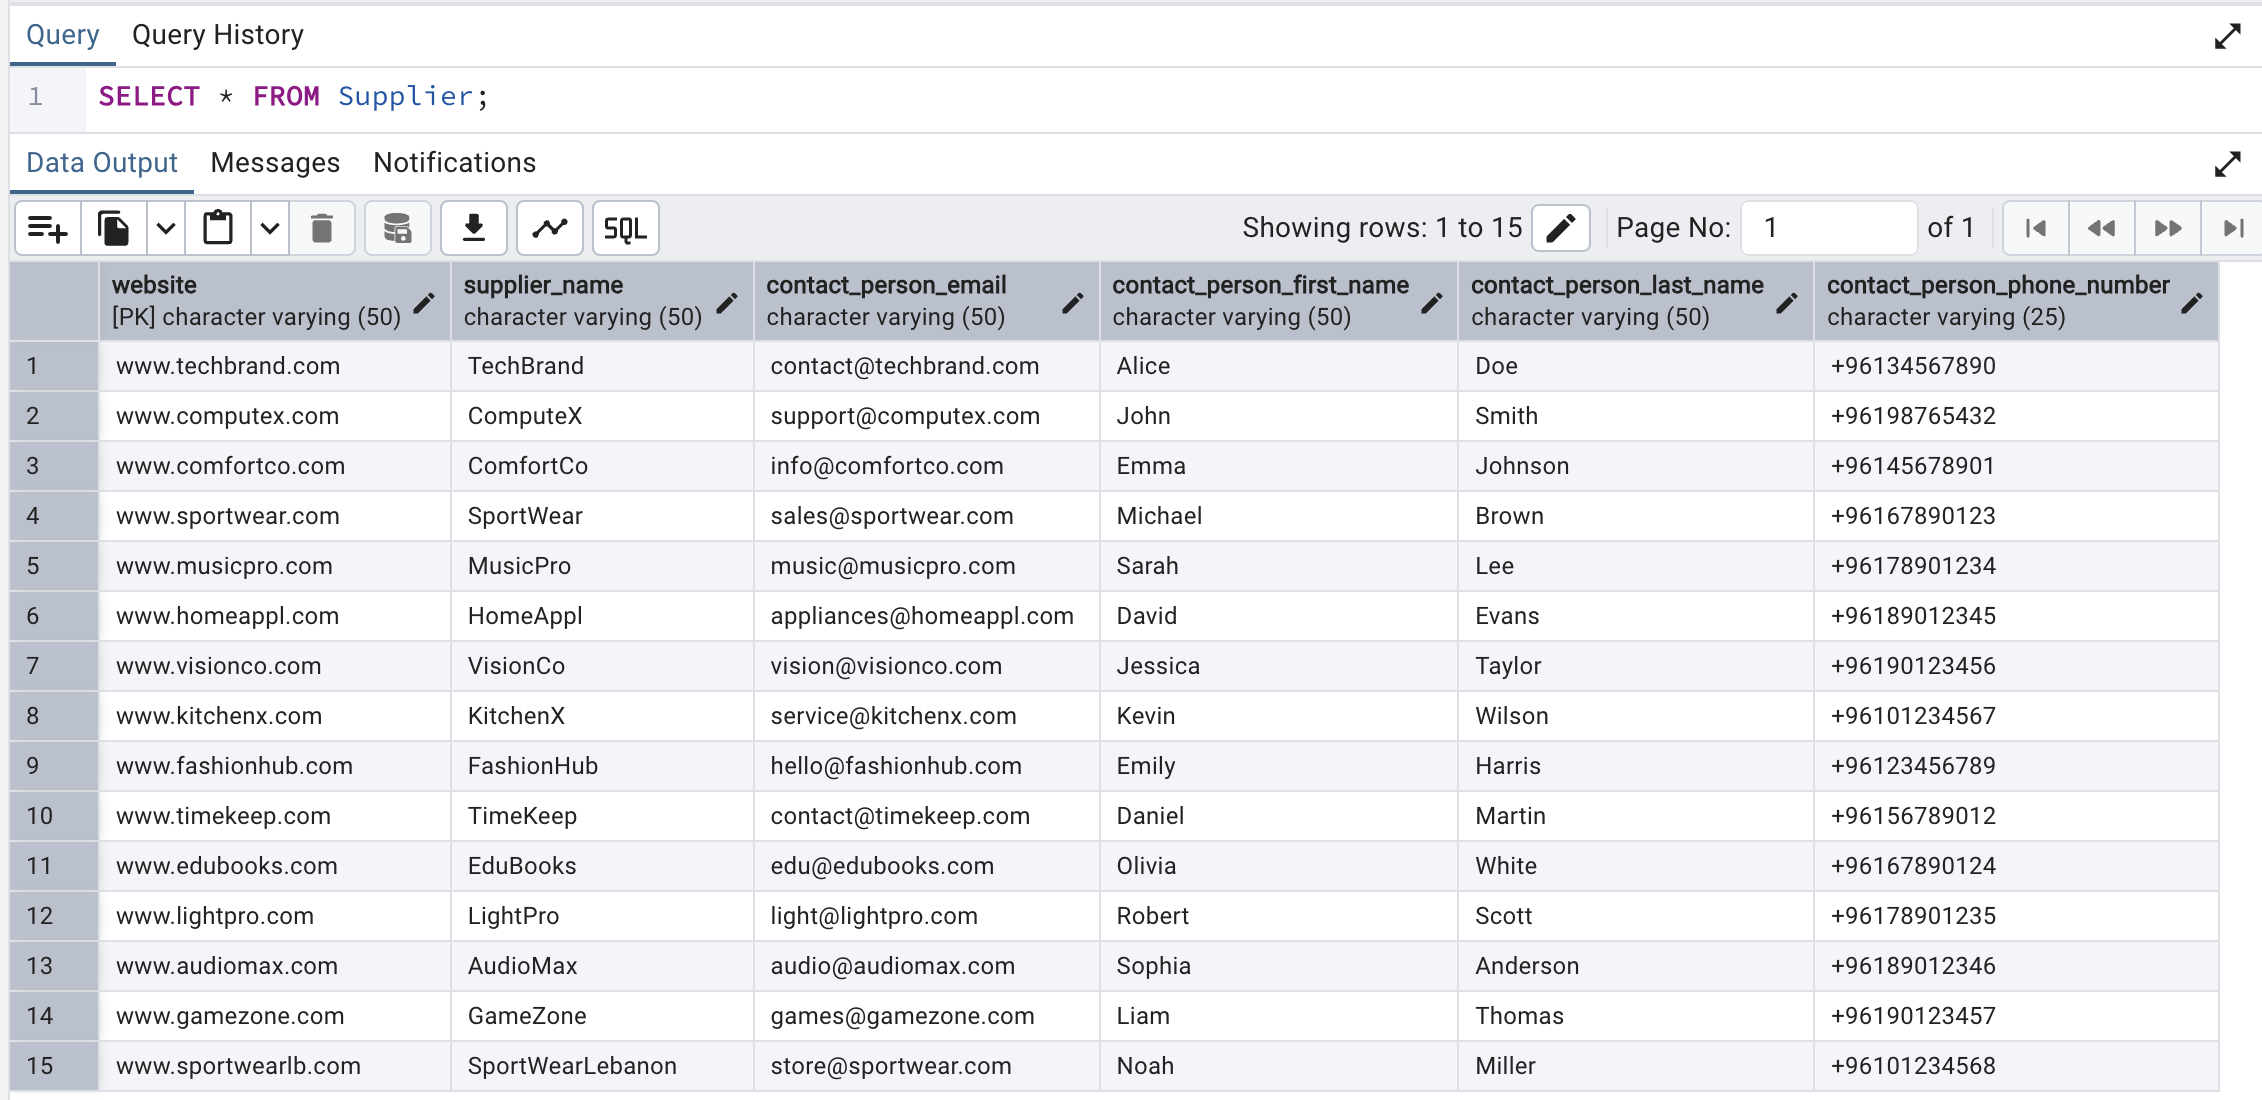
\includegraphics[width=1\textwidth]{images/sql/select/supplier.png}
  \caption{\textit{Select from Supplier Table}}
\end{figure}

\subsubsubsection{Category}
The following script selects data from the Category table.
\lstinputlisting[language=SQL, caption={\textit{Select from Category Table}}]{sql/select/category.sql}

\begin{figure}[H]
  \centering
  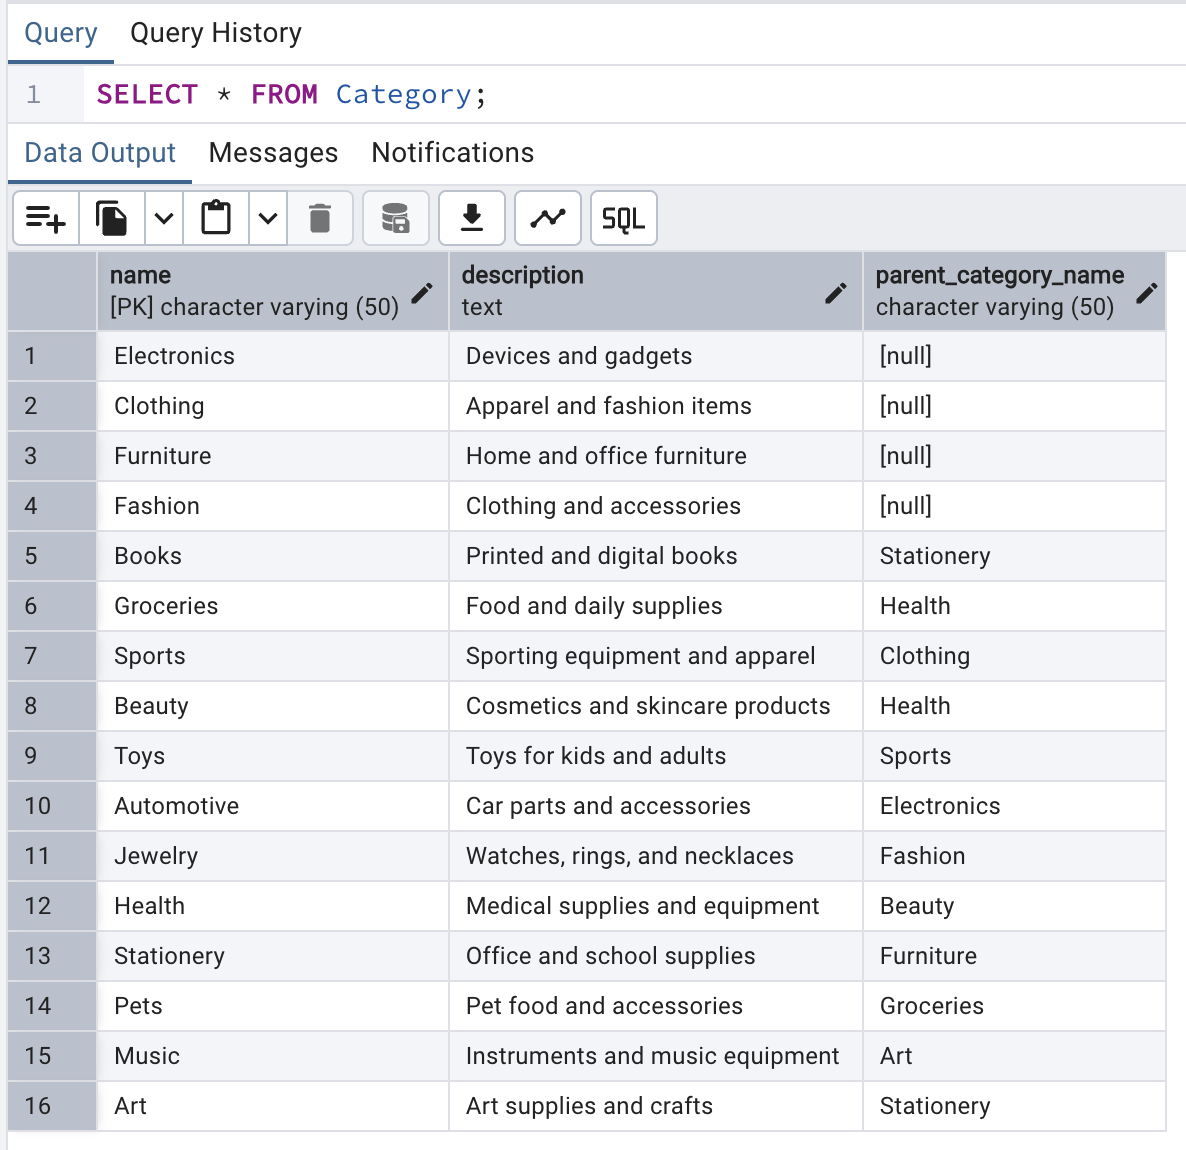
\includegraphics[width=1\textwidth]{images/sql/select/category.png}
  \caption{\textit{Select from Category Table}}
\end{figure}

\subsubsubsection{Product}
The following script selects data from the Product table.
\lstinputlisting[language=SQL, caption={\textit{Select from Product Table}}]{sql/select/product.sql}

\begin{figure}[H]
  \centering
  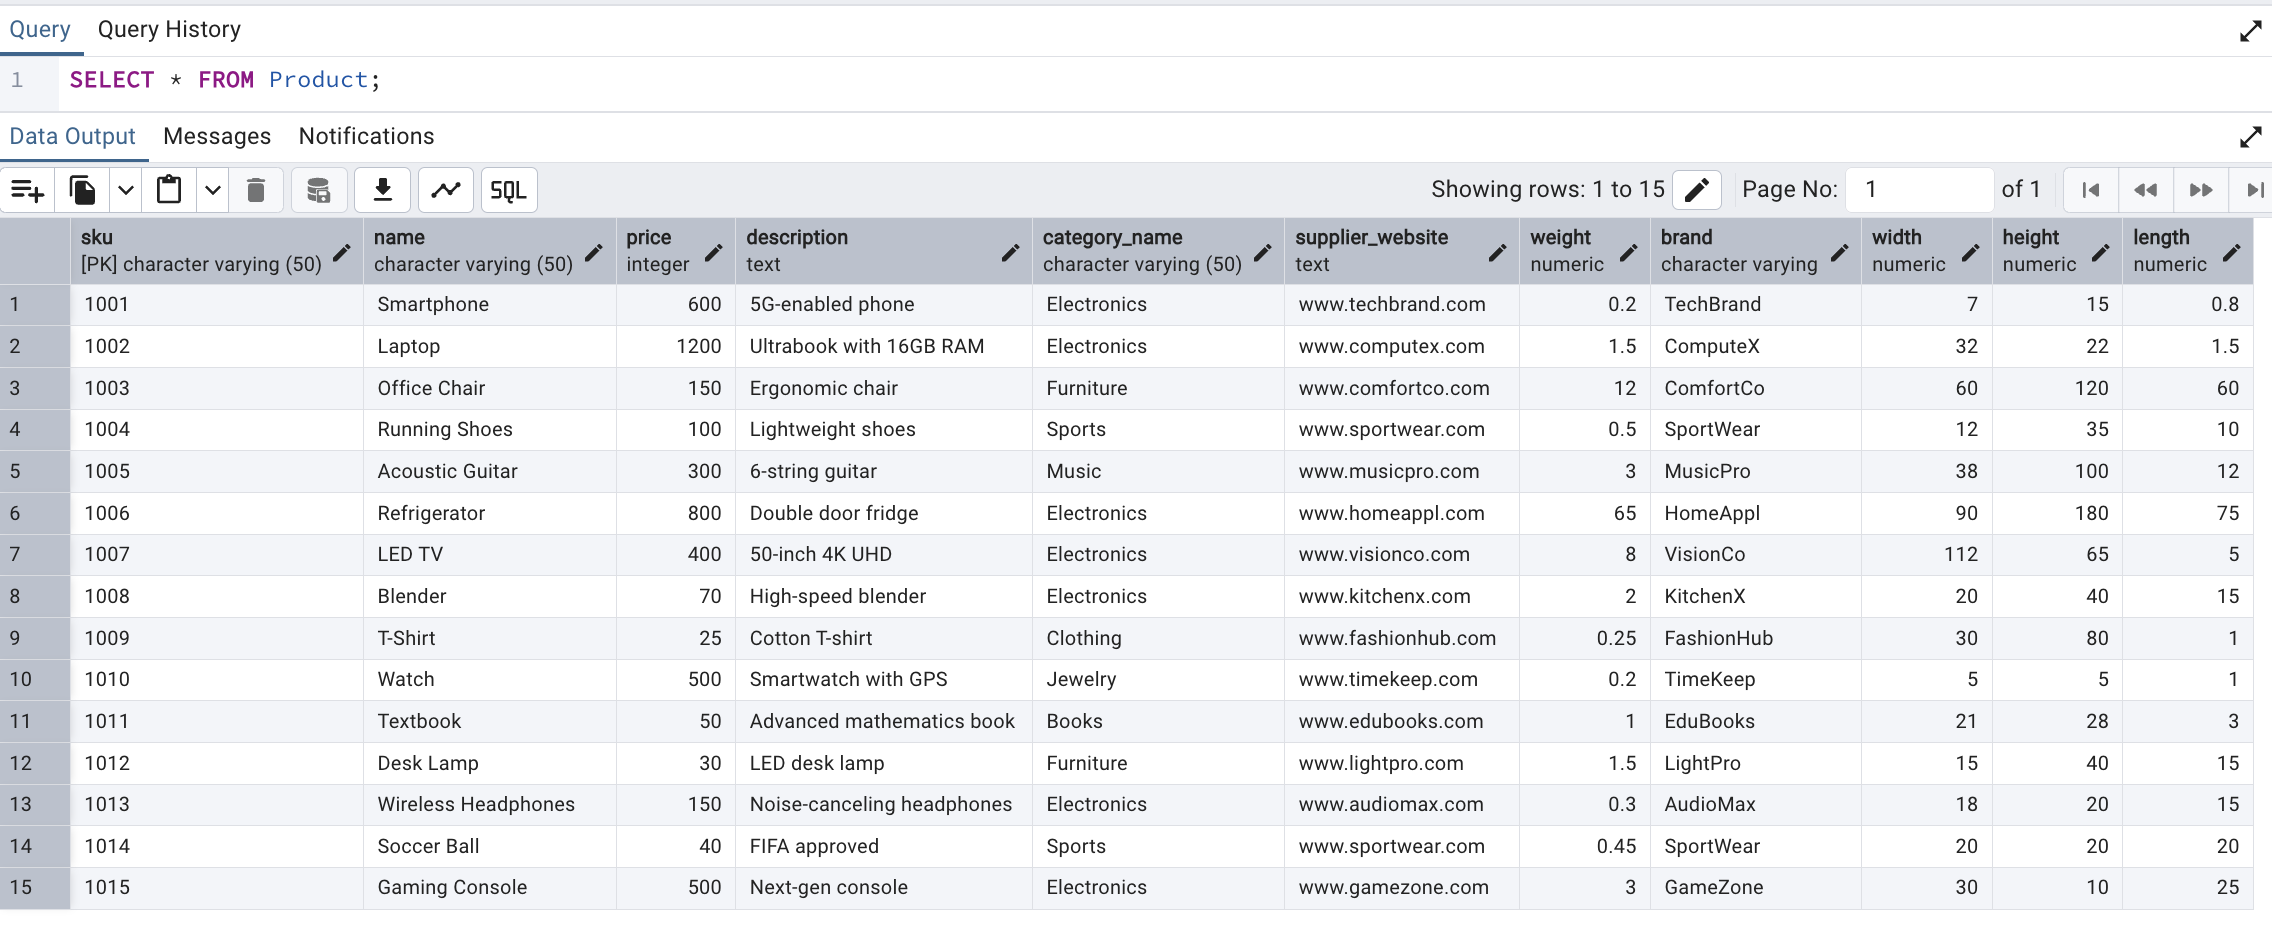
\includegraphics[width=1\textwidth]{images/sql/select/product.png}
  \caption{\textit{Select from Product Table}}
\end{figure}

\subsubsubsection{Branch}
The following script selects data from the Branch table.
\lstinputlisting[language=SQL, caption={\textit{Select from Branch Table}}]{sql/select/branch.sql}

\begin{figure}[H]
  \centering
  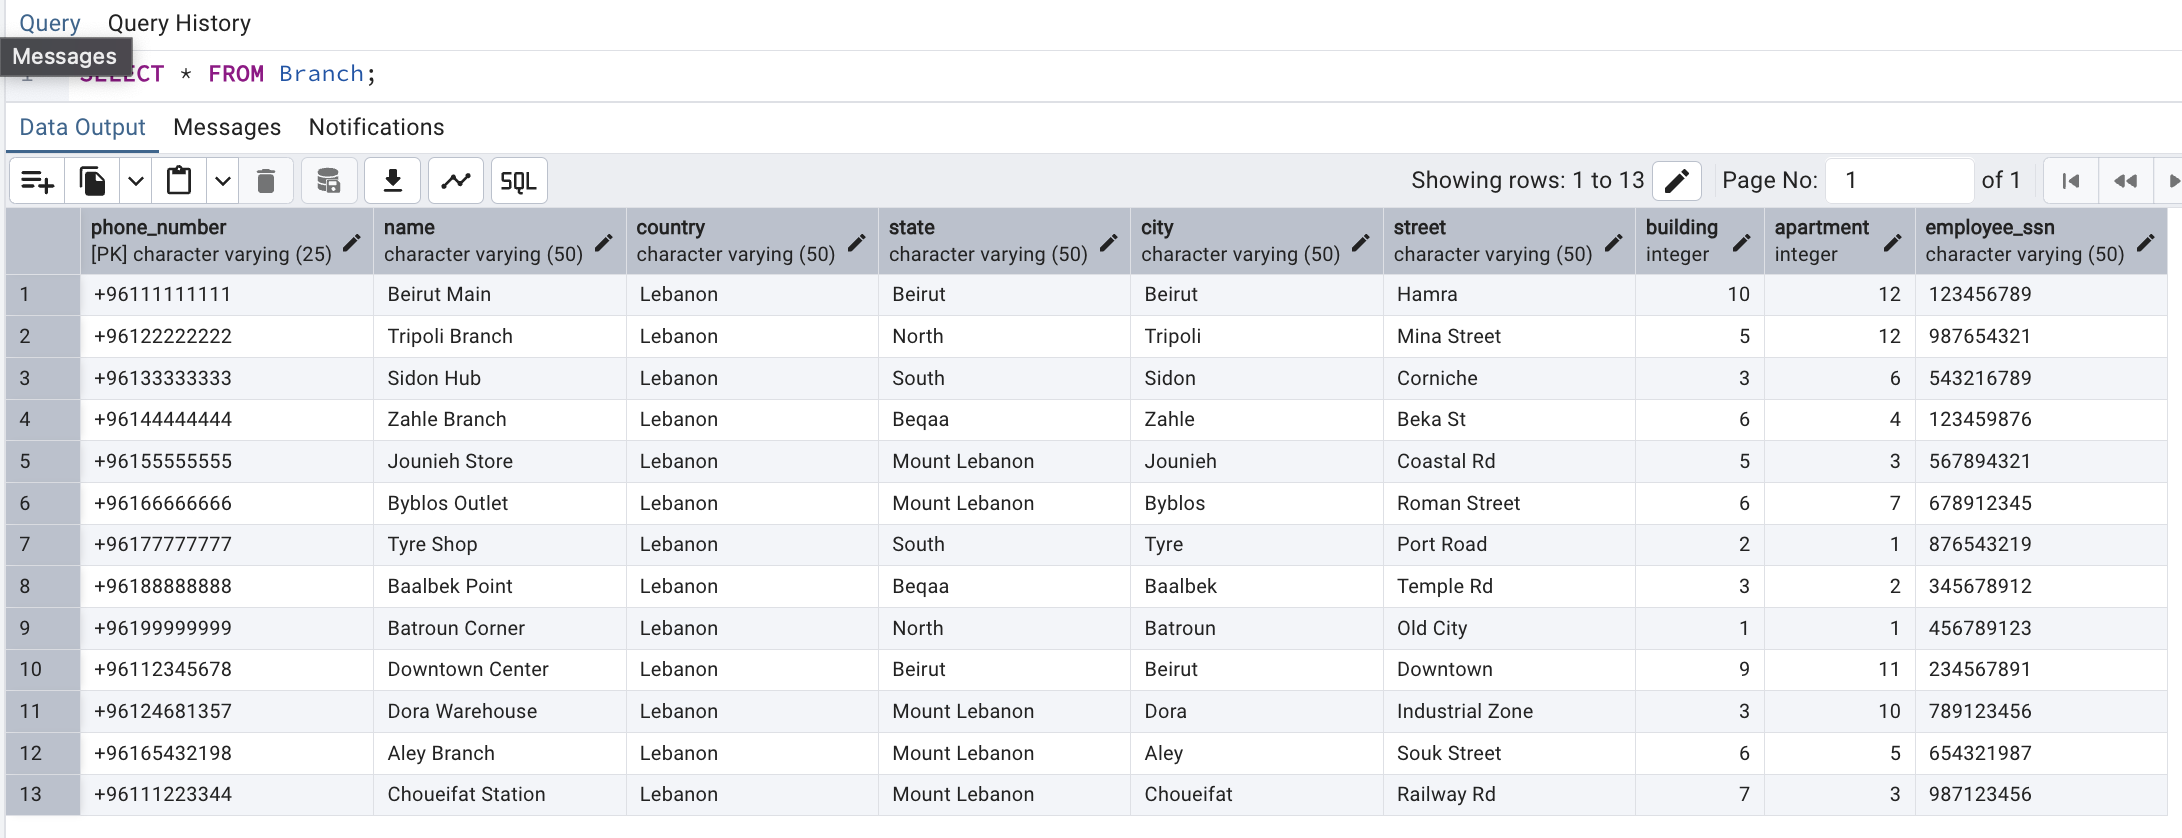
\includegraphics[width=1\textwidth]{images/sql/select/branch.png}
  \caption{\textit{Select from Branch Table}}
\end{figure}

\subsubsubsection{Department}
The following script selects data from the Department table.
\lstinputlisting[language=SQL, caption={\textit{Select from Department Table}}]{sql/select/department.sql}

\begin{figure}[H]
  \centering
  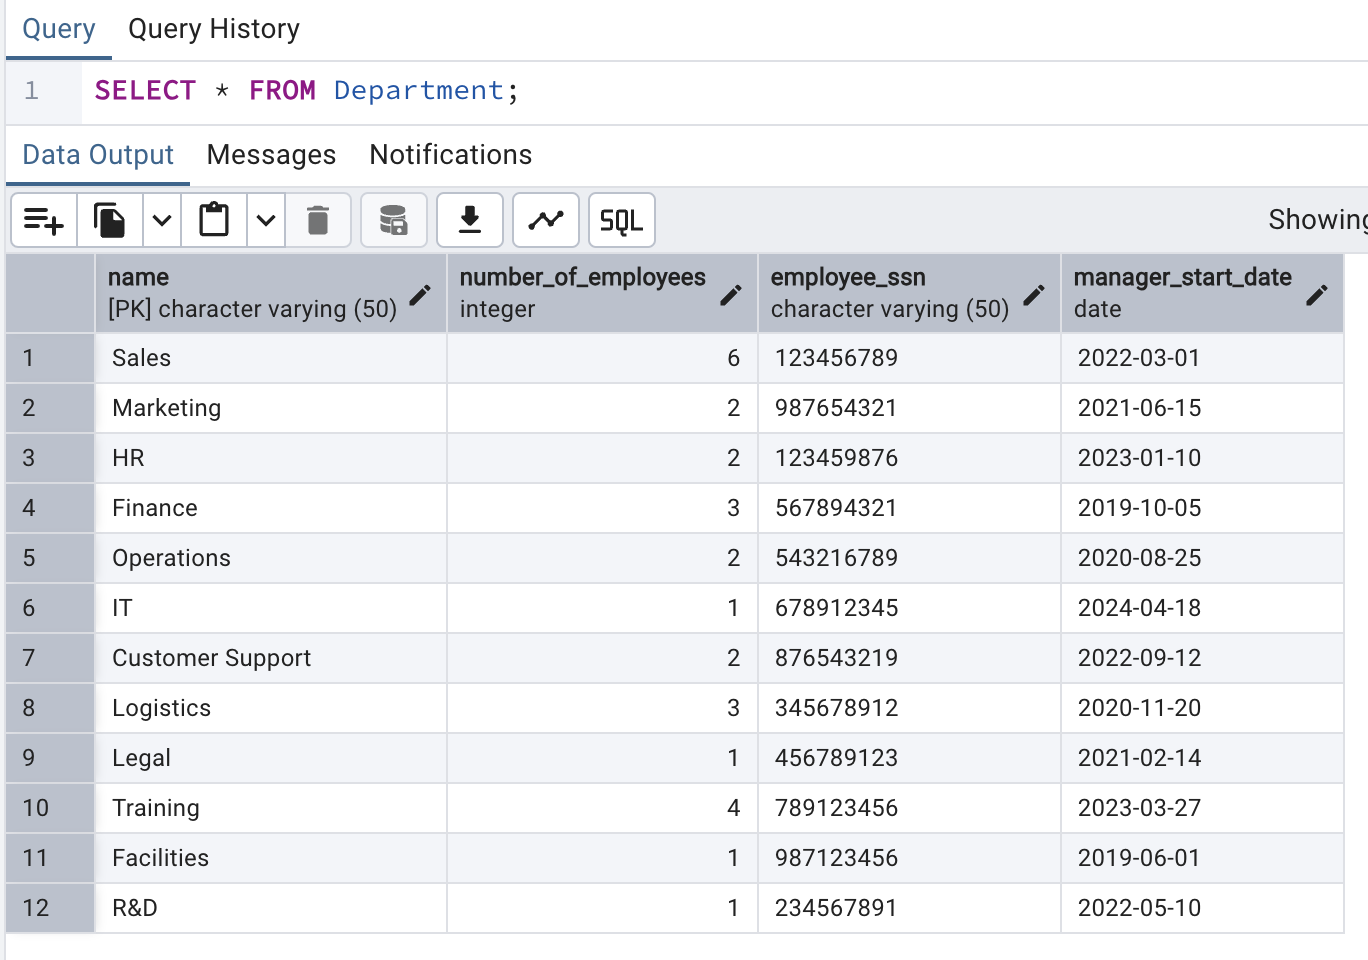
\includegraphics[width=1\textwidth]{images/sql/select/department.png}
  \caption{\textit{Select from Department Table}}
\end{figure}

\subsubsubsection{Employee}
The following script selects data from the Employee table.
\lstinputlisting[language=SQL, caption={\textit{Select from Employee Table}}]{sql/select/employee.sql}

\begin{figure}[H]
  \centering
  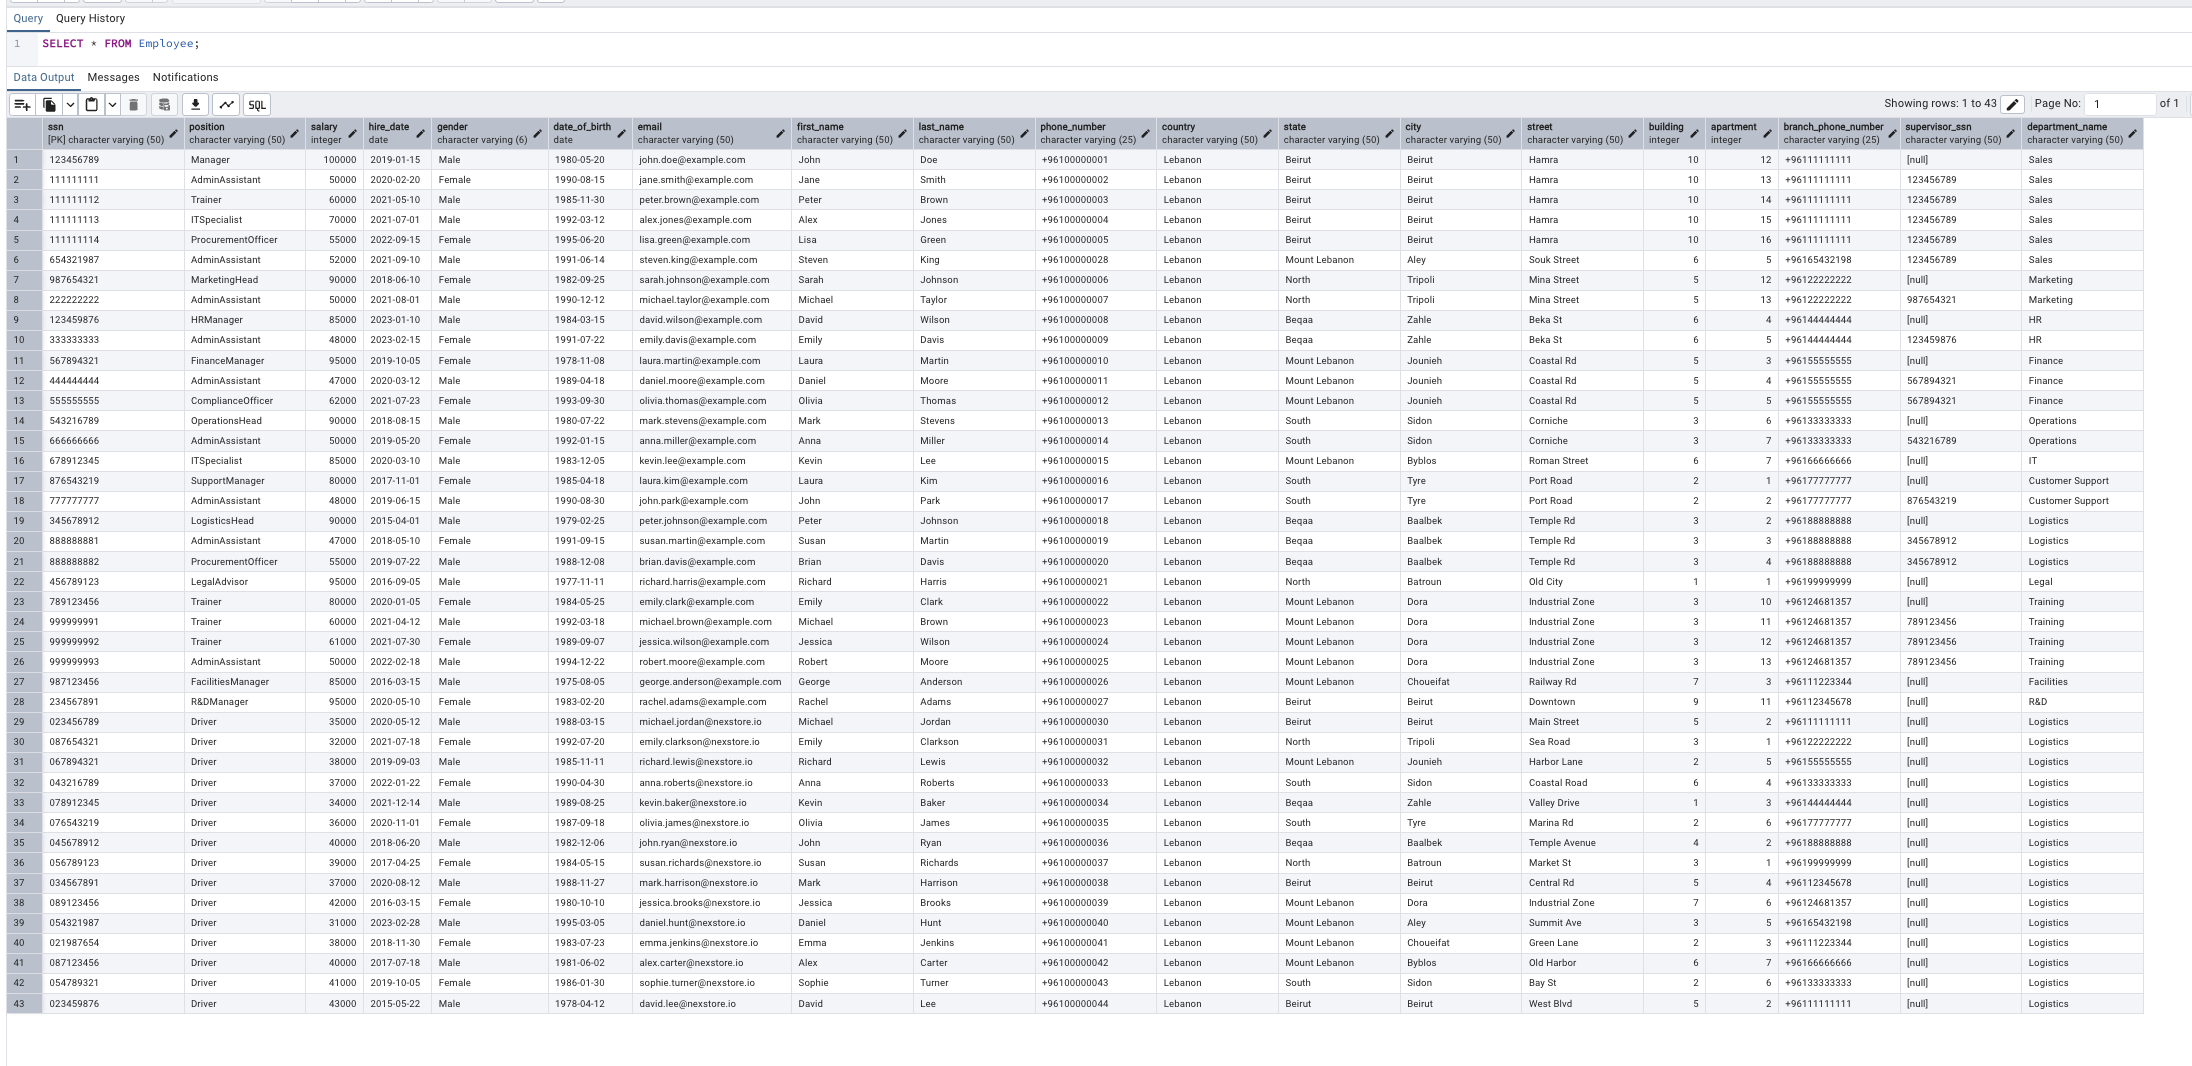
\includegraphics[width=1\textwidth]{images/sql/select/employee.png}
  \caption{\textit{Select from Employee Table}}
\end{figure}

\subsubsubsection{Driver}
The following script selects data from the Driver table.
\lstinputlisting[language=SQL, caption={\textit{Select from Driver Table}}]{sql/select/driver.sql}

\begin{figure}[H]
  \centering
  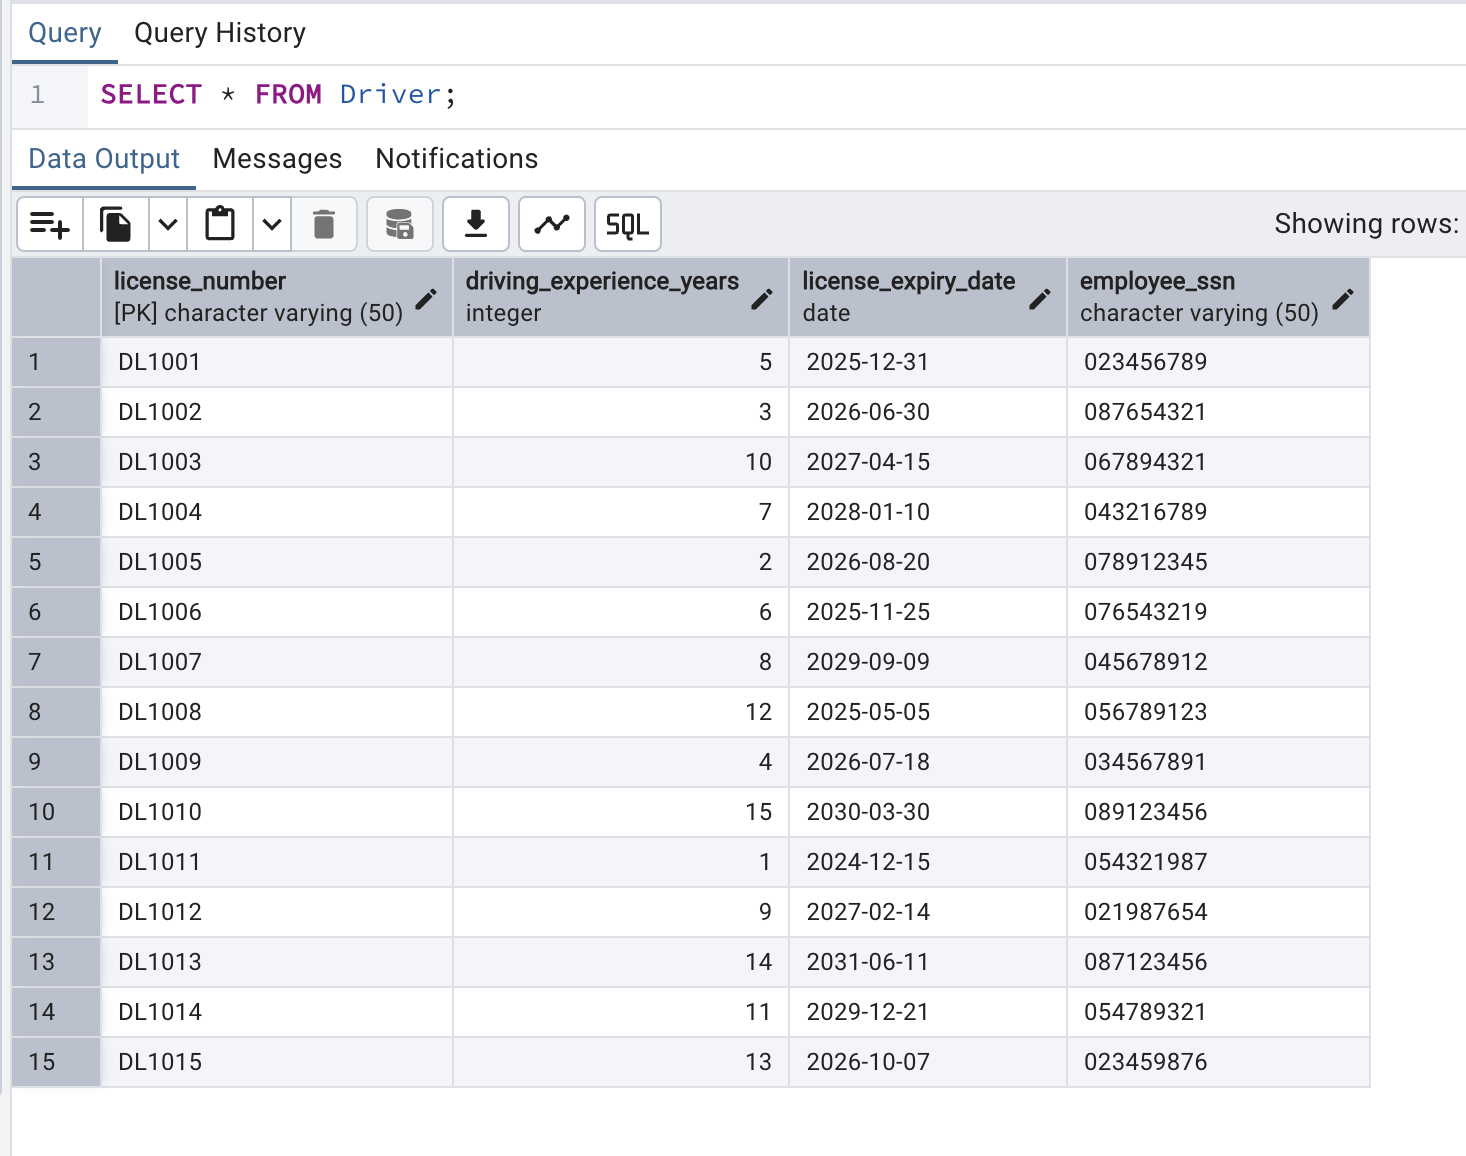
\includegraphics[width=1\textwidth]{images/sql/select/driver.png}
  \caption{\textit{Select from Driver Table}}
\end{figure}

\subsubsubsection{Customer}
The following script selects data from the Customer table.
\lstinputlisting[language=SQL, caption={\textit{Select from Customer Table}}]{sql/select/customer.sql}

\begin{figure}[H]
  \centering
  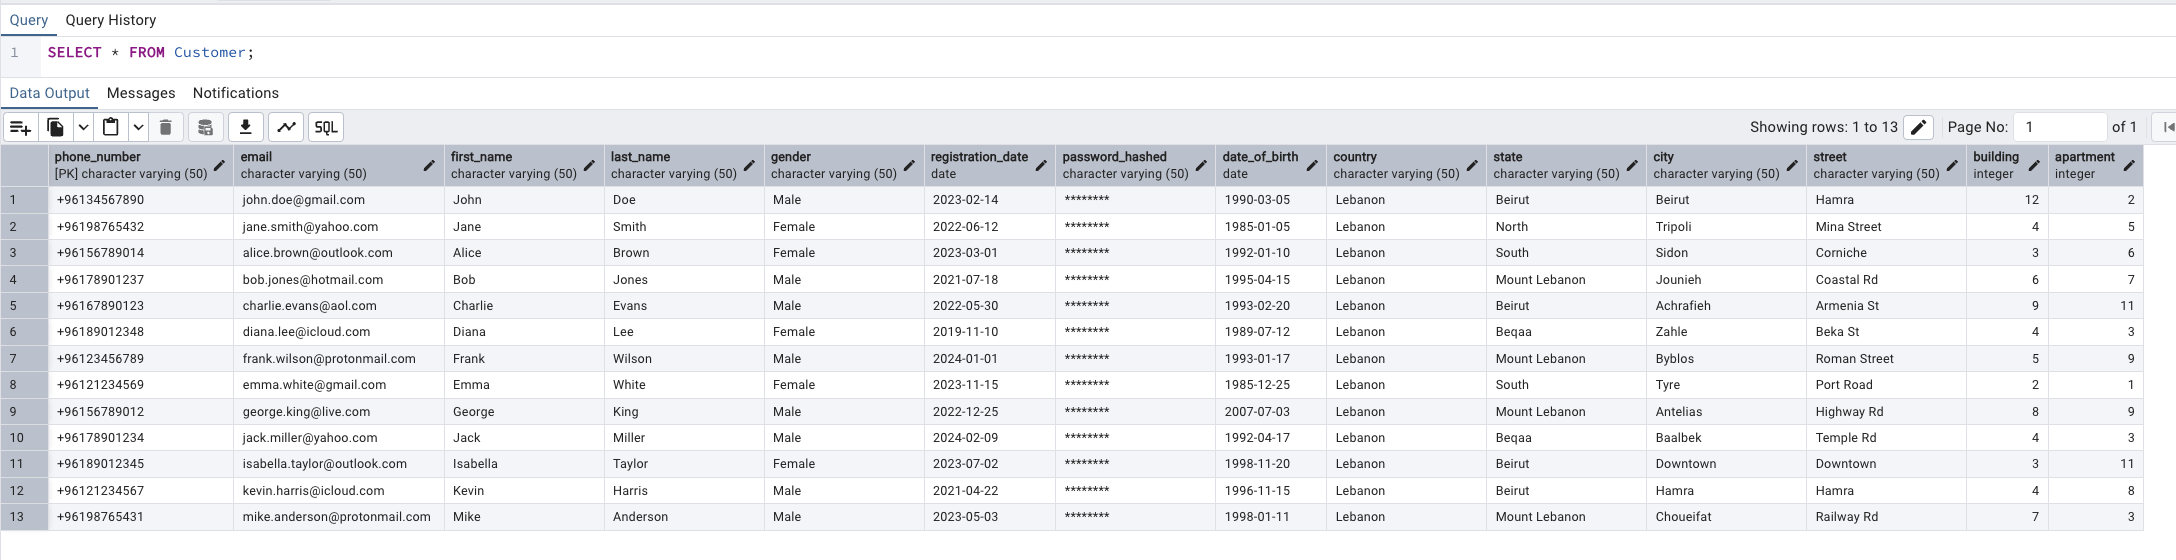
\includegraphics[width=1\textwidth]{images/sql/select/customer.png}
  \caption{\textit{Select from Customer Table}}
\end{figure}

\subsubsubsection{Orders}
The following script selects data from the Orders table.
\lstinputlisting[language=SQL, caption={\textit{Select from Orders Table}}]{sql/select/orders.sql}

\begin{figure}[H]
  \centering
  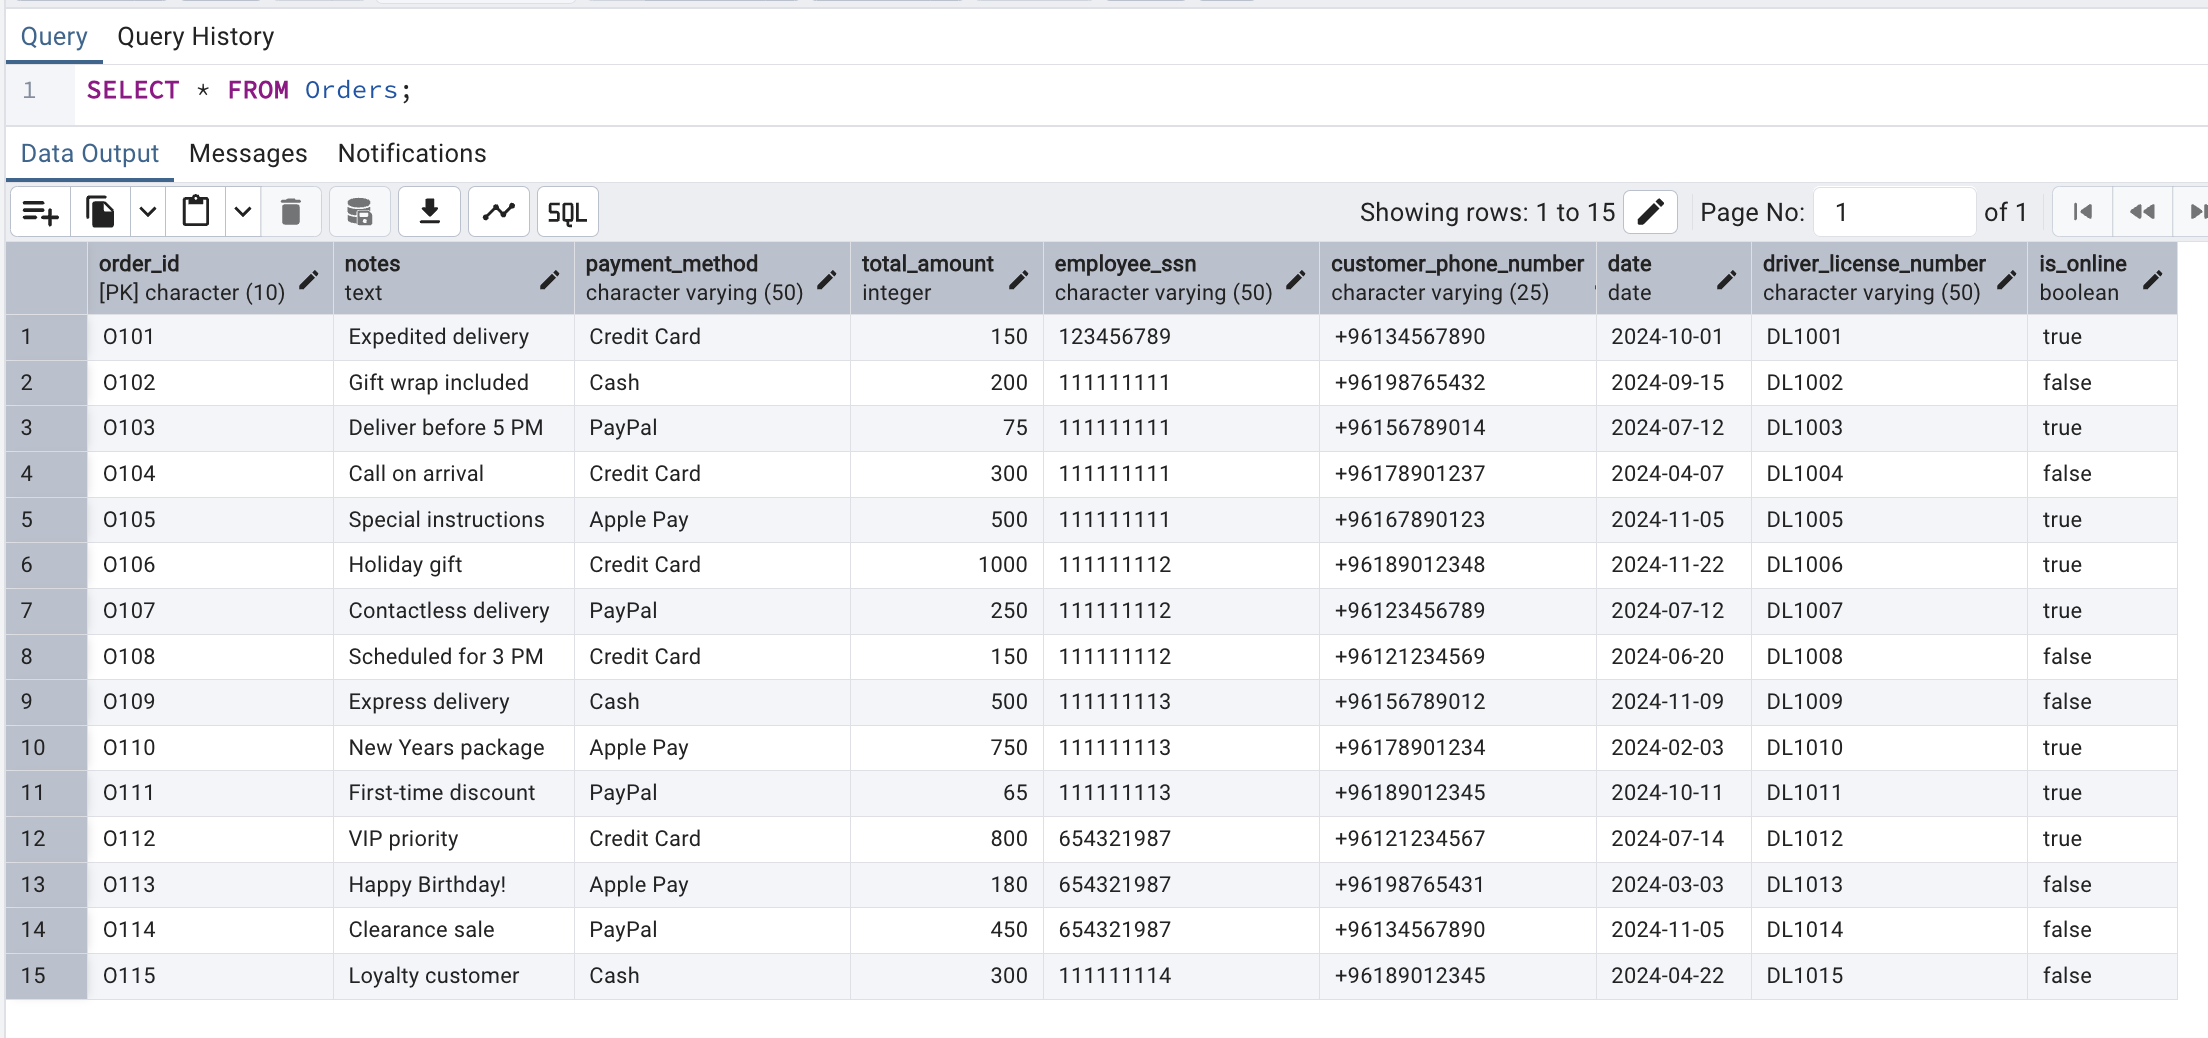
\includegraphics[width=1\textwidth]{images/sql/select/orders.png}
  \caption{\textit{Select from Orders Table}}
\end{figure}

\subsubsubsection{Purchased}
The following script selects data from the Purchased table.
\lstinputlisting[language=SQL, caption={\textit{Select from Purchased Table}}]{sql/select/purchased.sql}

\begin{figure}[H]
  \centering
  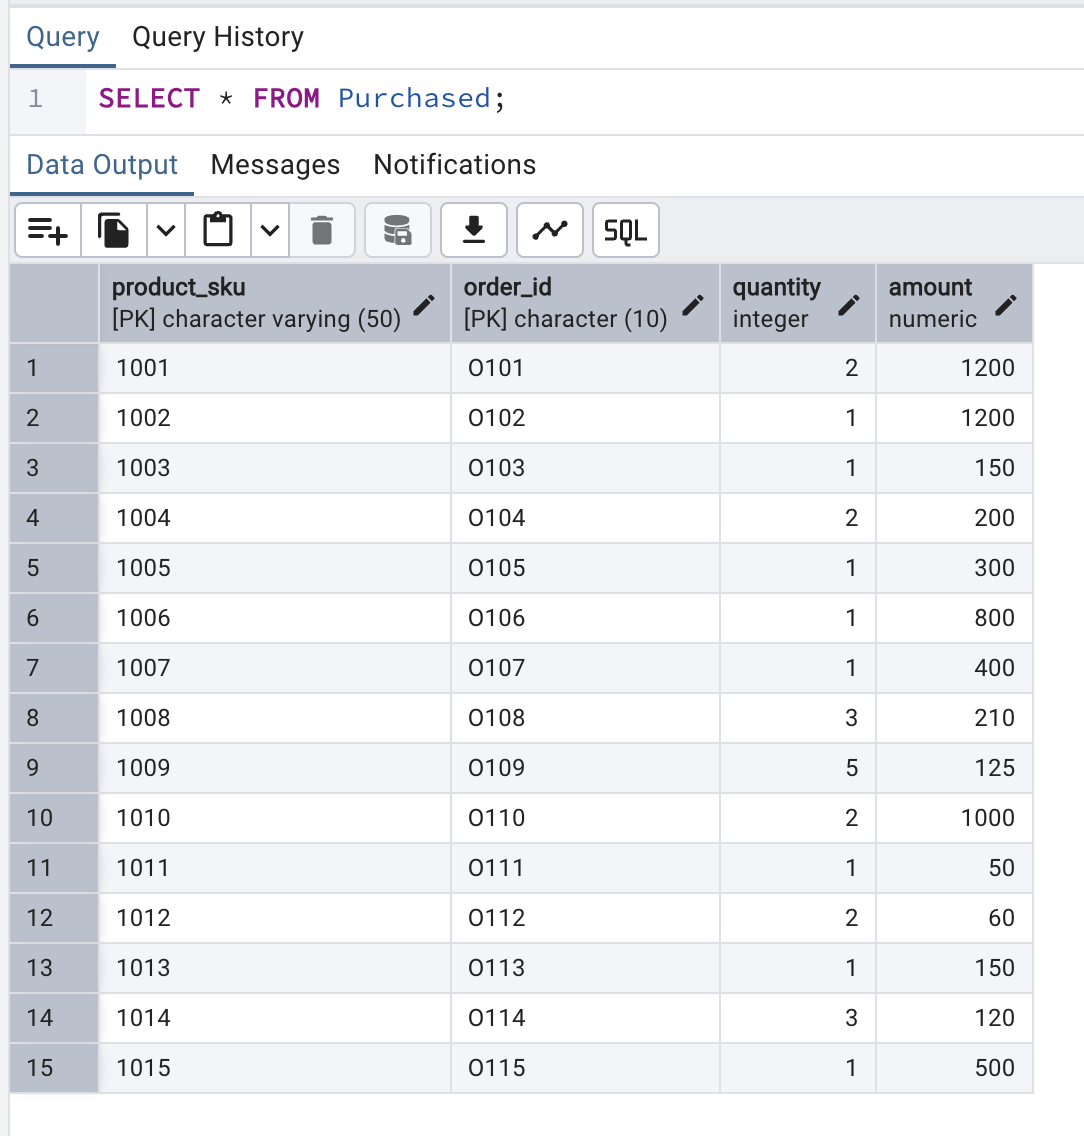
\includegraphics[width=1\textwidth]{images/sql/select/purchased.png}
  \caption{\textit{Select from Purchased Table}}
\end{figure}

\subsubsubsection{Reviews}
The following script selects data from the Reviews table.
\lstinputlisting[language=SQL, caption={\textit{Select from Reviews Table}}]{sql/select/reviews.sql}

\begin{figure}[H]
  \centering
  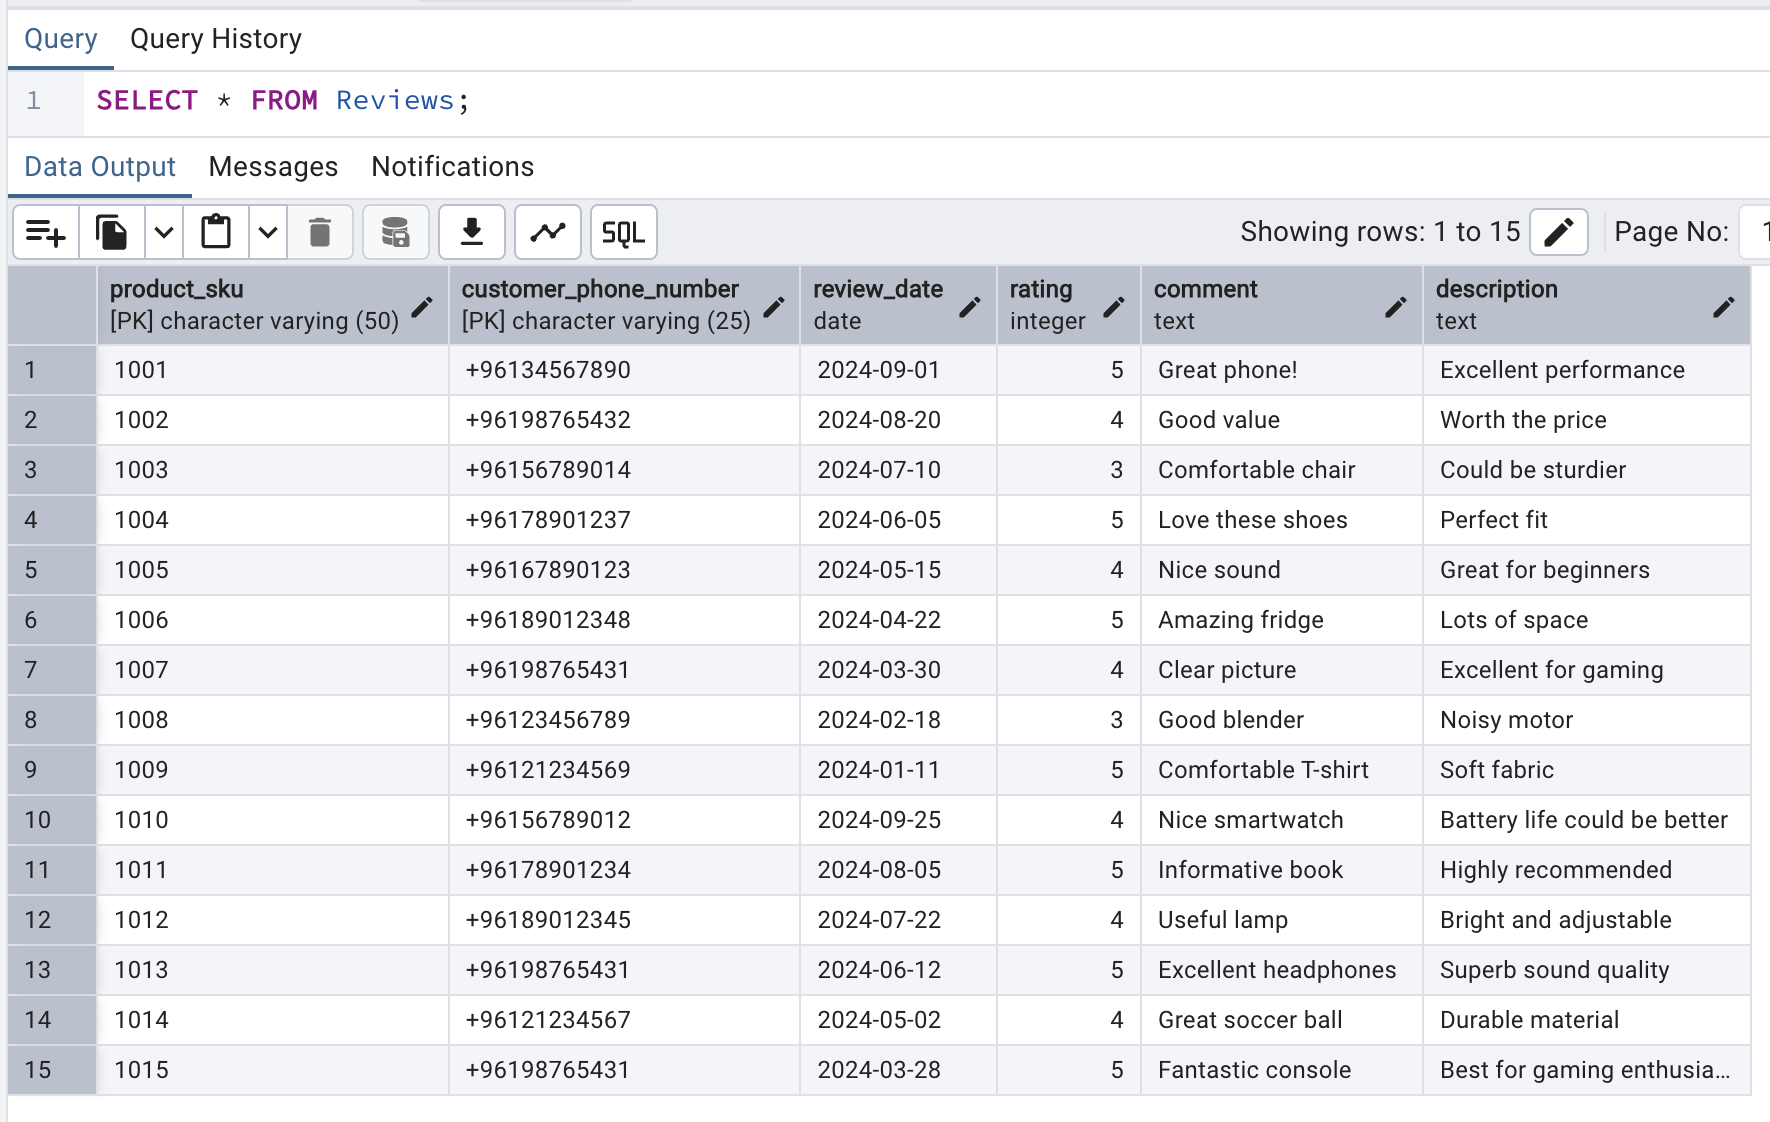
\includegraphics[width=1\textwidth]{images/sql/select/reviews.png}
  \caption{\textit{Select from Reviews Table}}
\end{figure}

\subsubsubsection{Support Ticket}
The following script selects data from the Support Ticket table.
\lstinputlisting[language=SQL, caption={\textit{Select from Support Ticket Table}}]{sql/select/support_ticket.sql}

\begin{figure}[H]
  \centering
  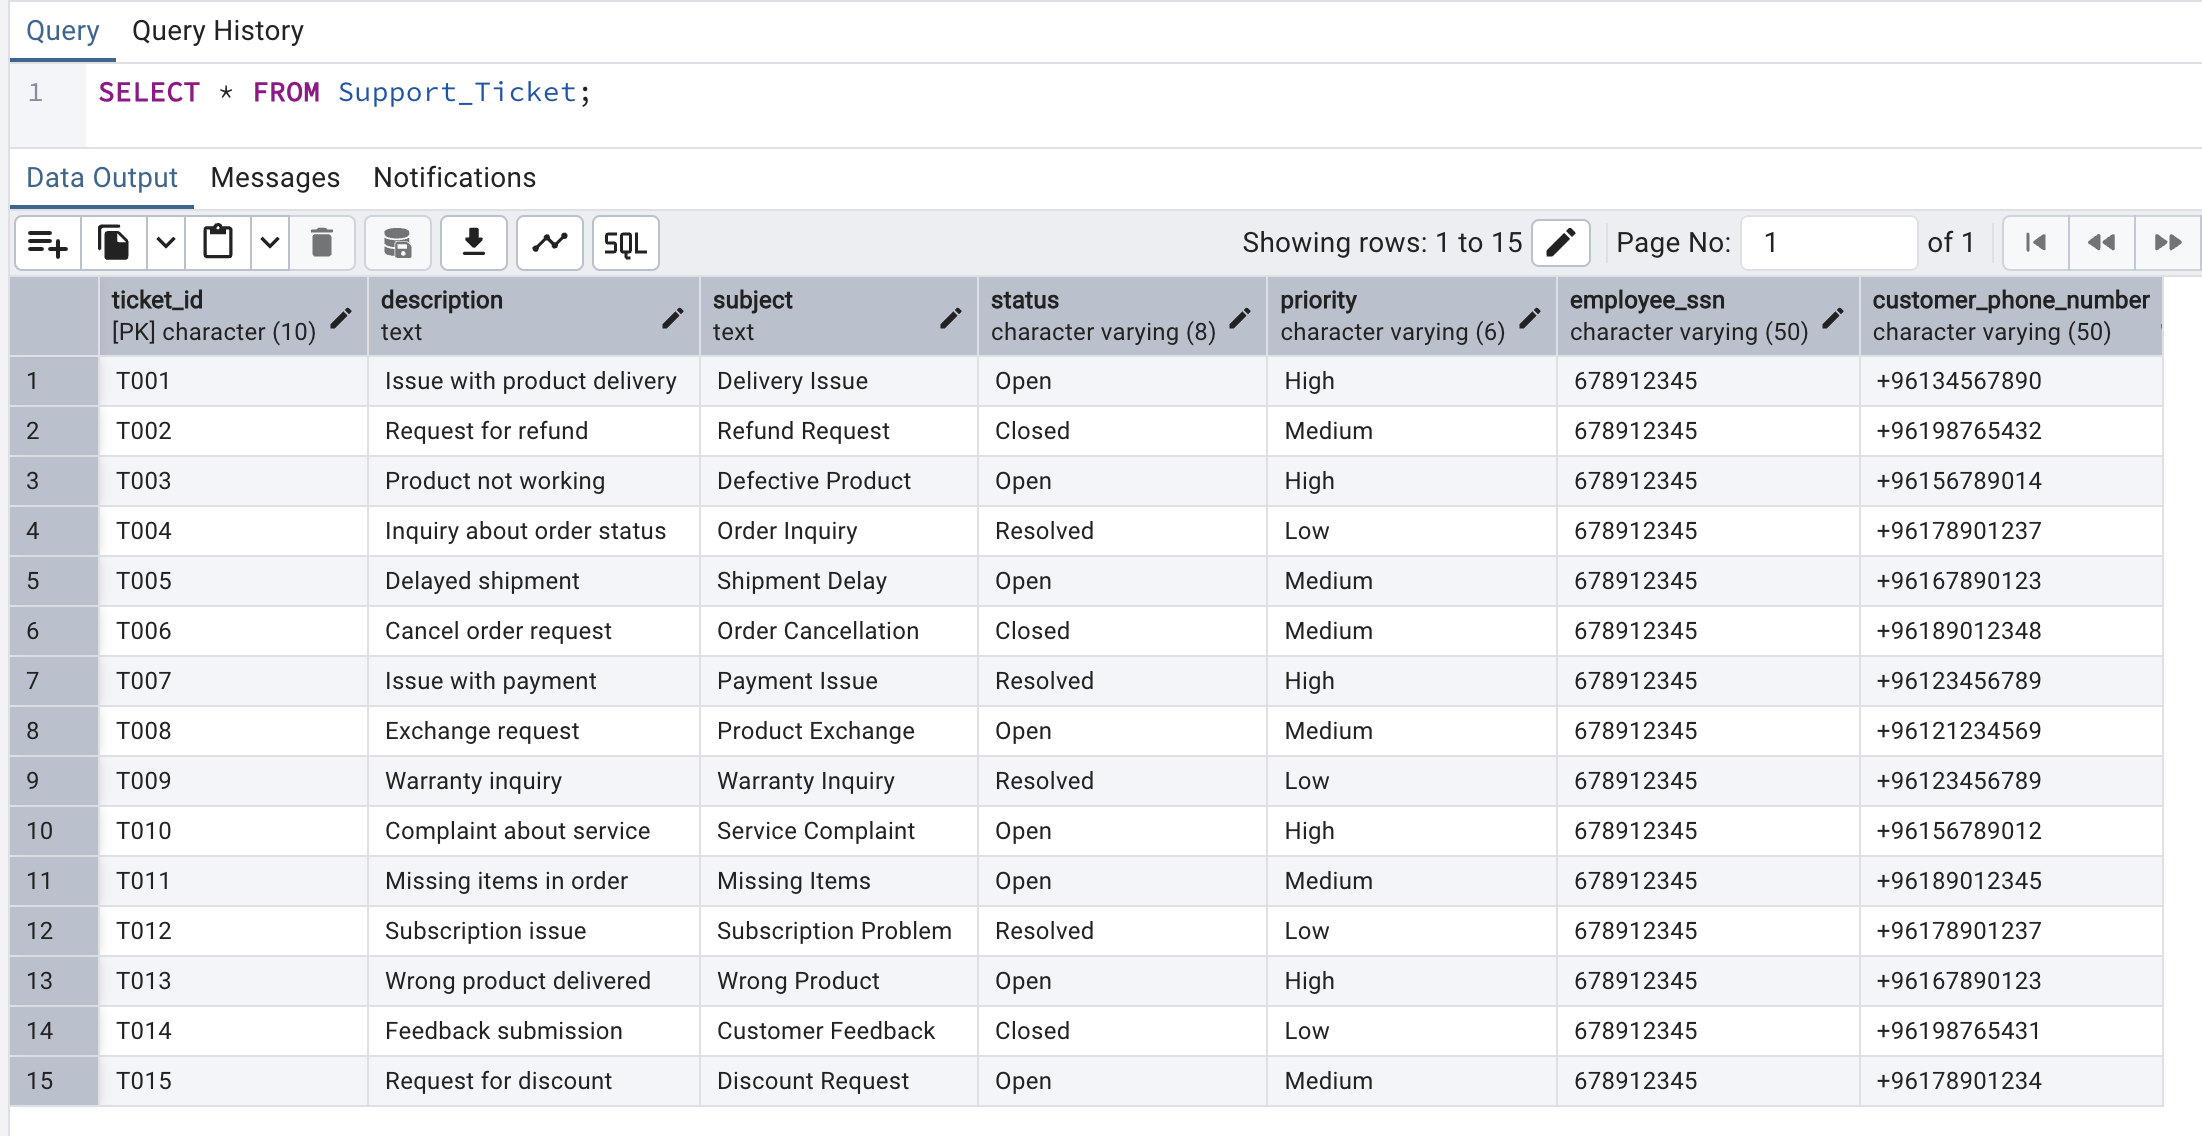
\includegraphics[width=1\textwidth]{images/sql/select/support_ticket.png}
  \caption{\textit{Select from Support Ticket Table}}
\end{figure}

\subsubsubsection{Wishlist}
The following script selects data from the Wishlist table.
\lstinputlisting[language=SQL, caption={\textit{Select from Wishlist Table}}]{sql/select/wishlist.sql}

\begin{figure}[H]
  \centering
  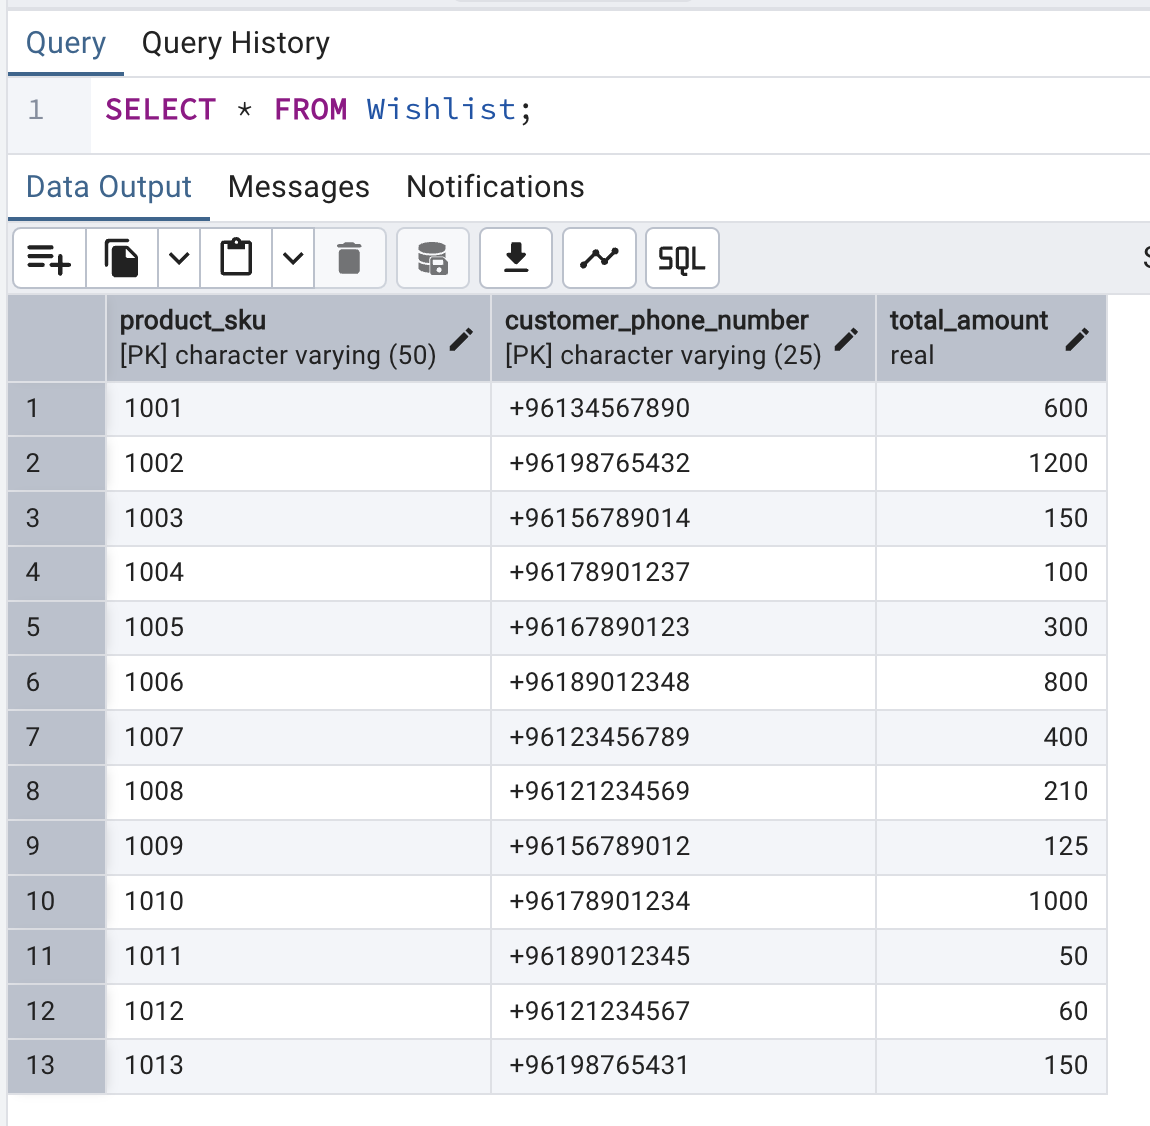
\includegraphics[width=1\textwidth]{images/sql/select/wishlist.png}
  \caption{\textit{Select from Wishlist Table}}
\end{figure}

\subsubsubsection{Working Hours}
The following script selects data from the Working Hours table.
\lstinputlisting[language=SQL, caption={\textit{Select from Working Hours Table}}]{sql/select/working_hours.sql}

\begin{figure}[H]
  \centering
  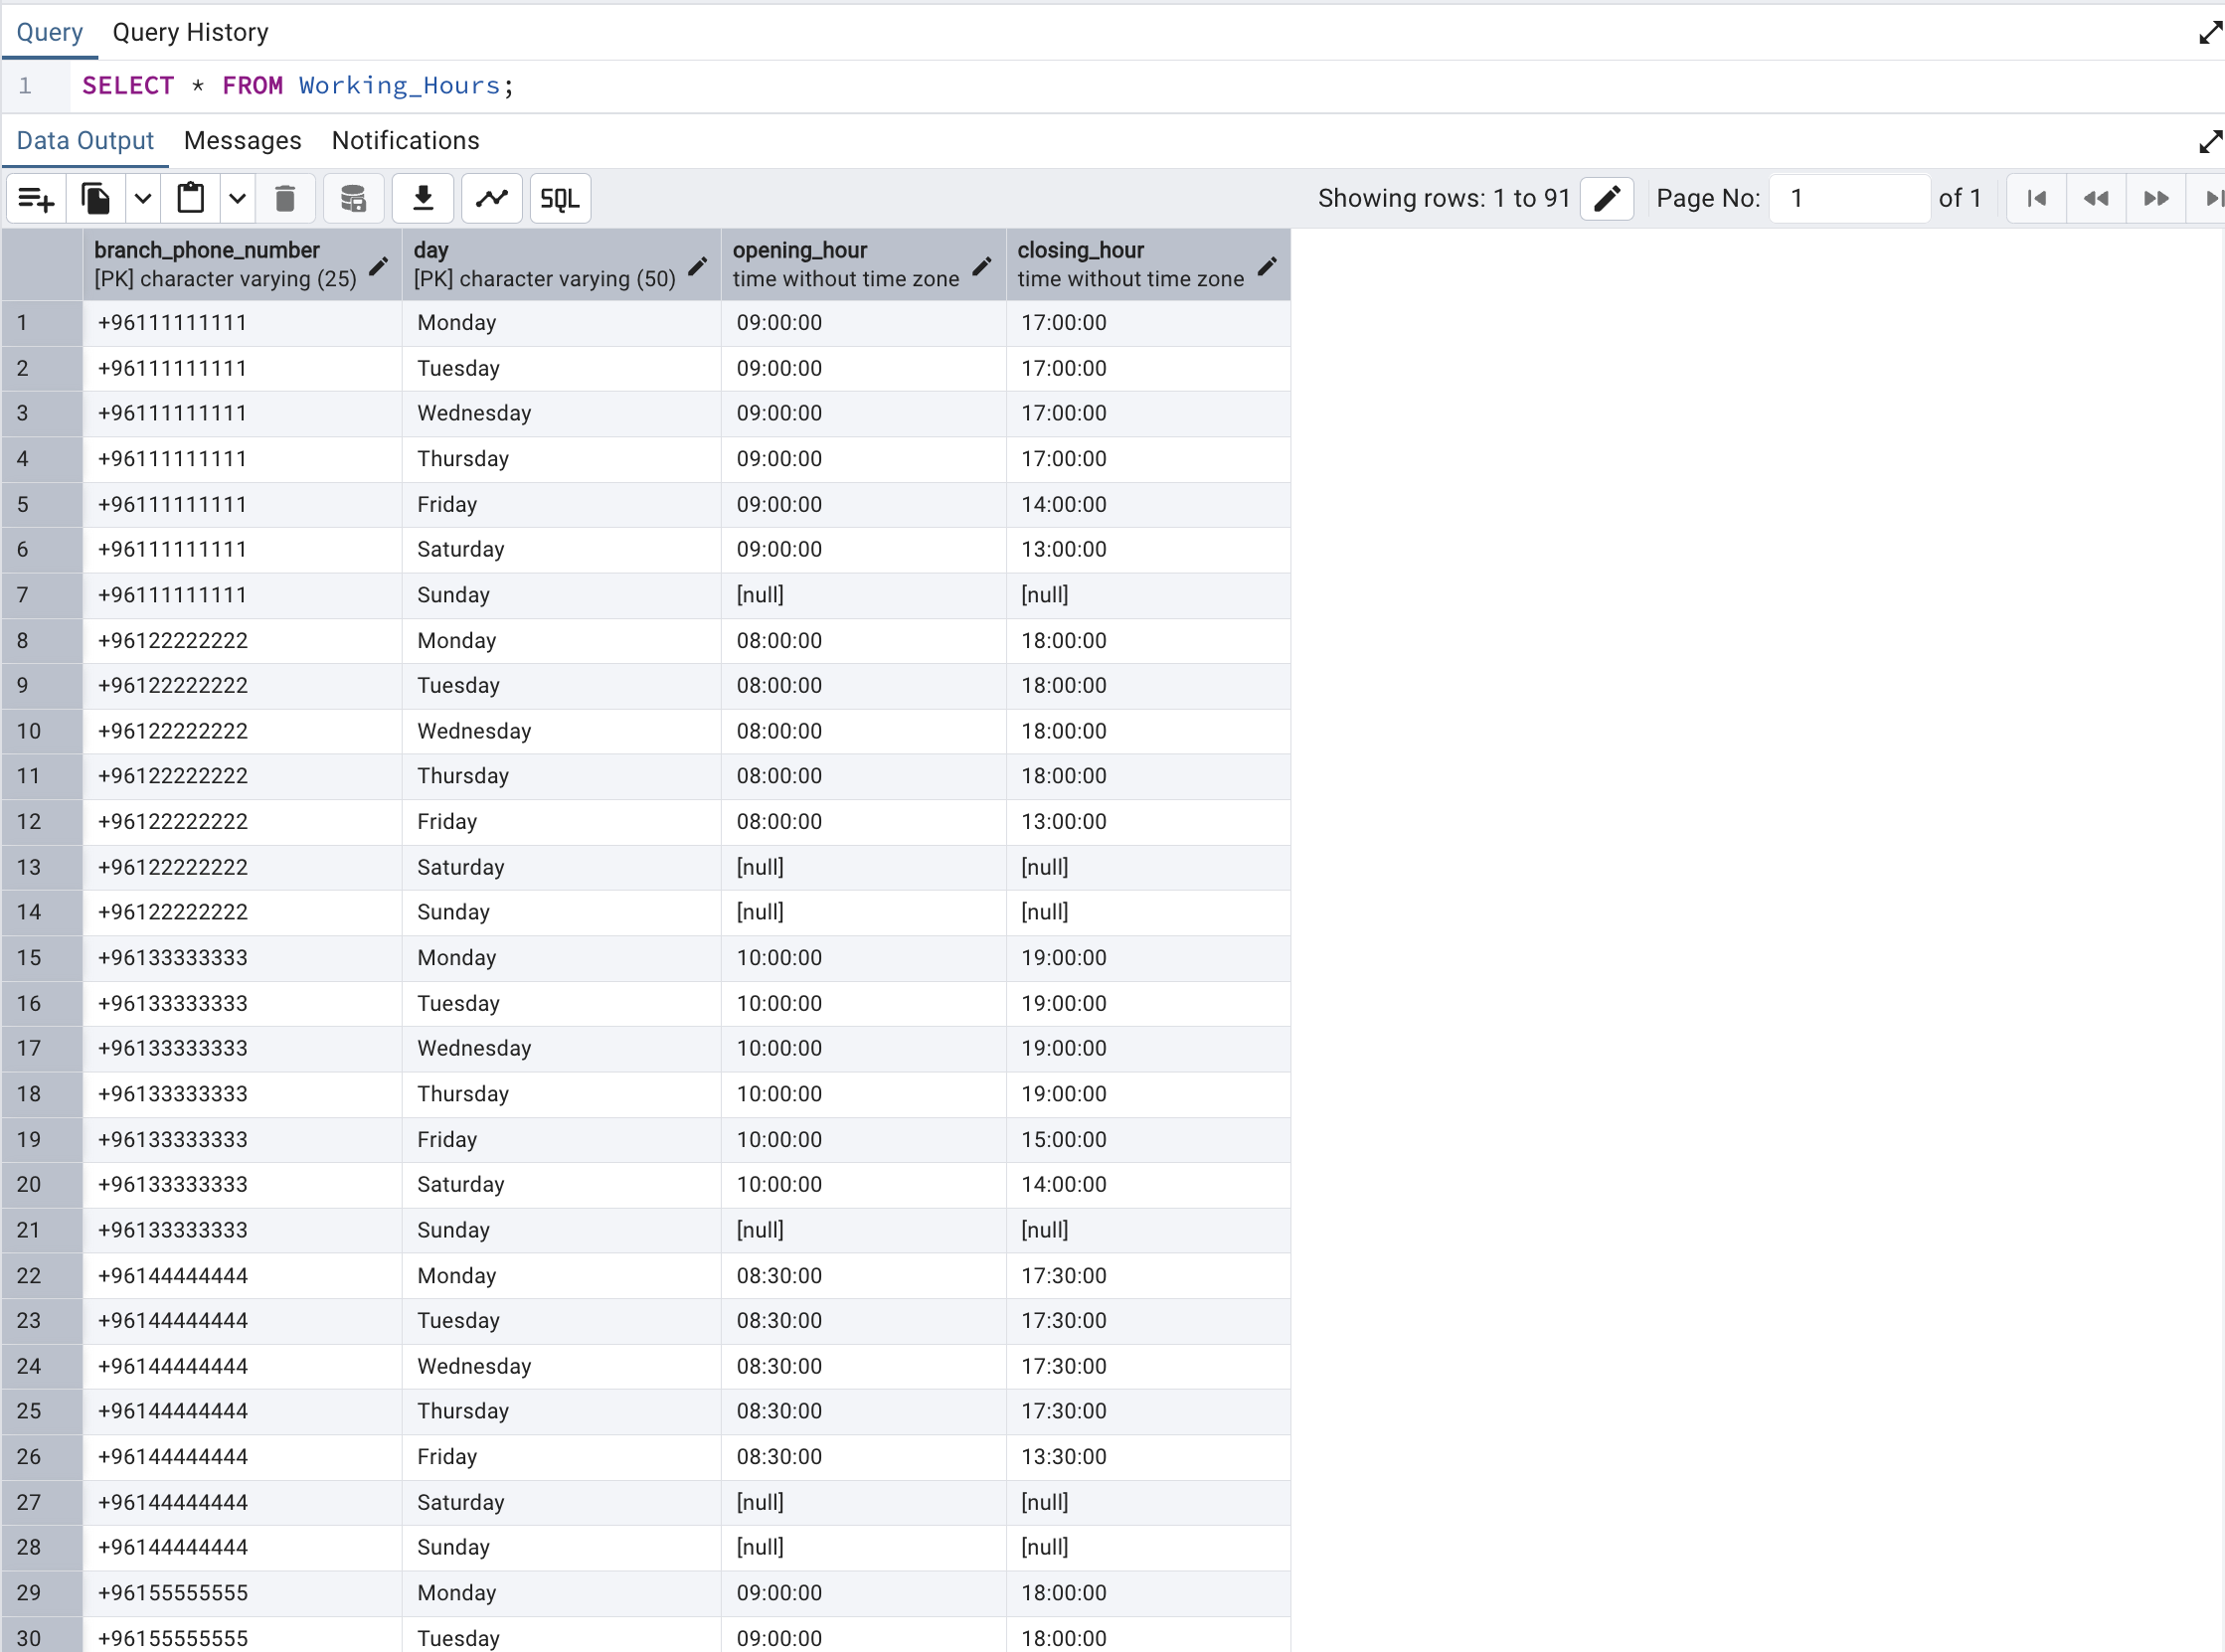
\includegraphics[width=1\textwidth]{images/sql/select/working_hours.png}
  \caption{\textit{Select from Working Hours Table}}
\end{figure}

\subsubsubsection{Dependent}
The following script selects data from the Dependent table.
\lstinputlisting[language=SQL, caption={\textit{Select from Dependent Table}}]{sql/select/dependent.sql}

\begin{figure}[H]
  \centering
  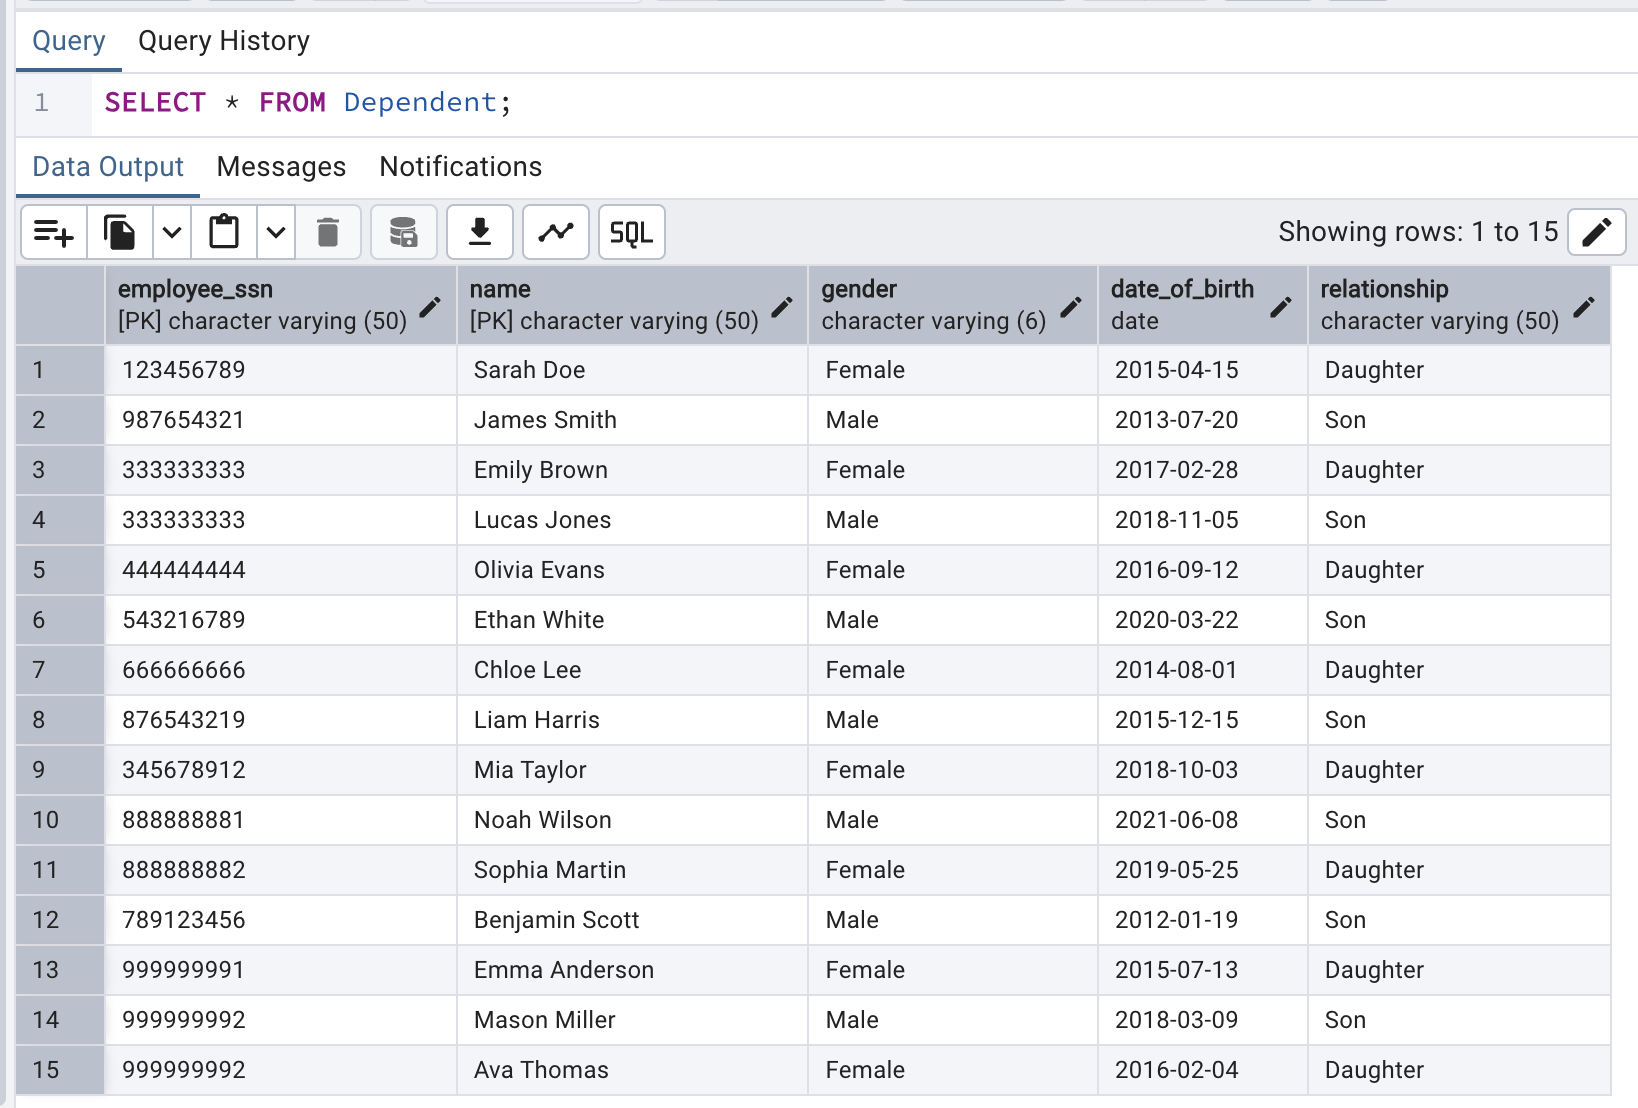
\includegraphics[width=1\textwidth]{images/sql/select/dependent.png}
  \caption{\textit{Select from Dependent Table}}
\end{figure}

\subsubsubsection{Product Image URLs}
The following script selects data from the Product Image URLs table.
\lstinputlisting[language=SQL, caption={\textit{Select from Product Image URLs Table}}]{sql/select/product_image_urls.sql}

\begin{figure}[H]
  \centering
  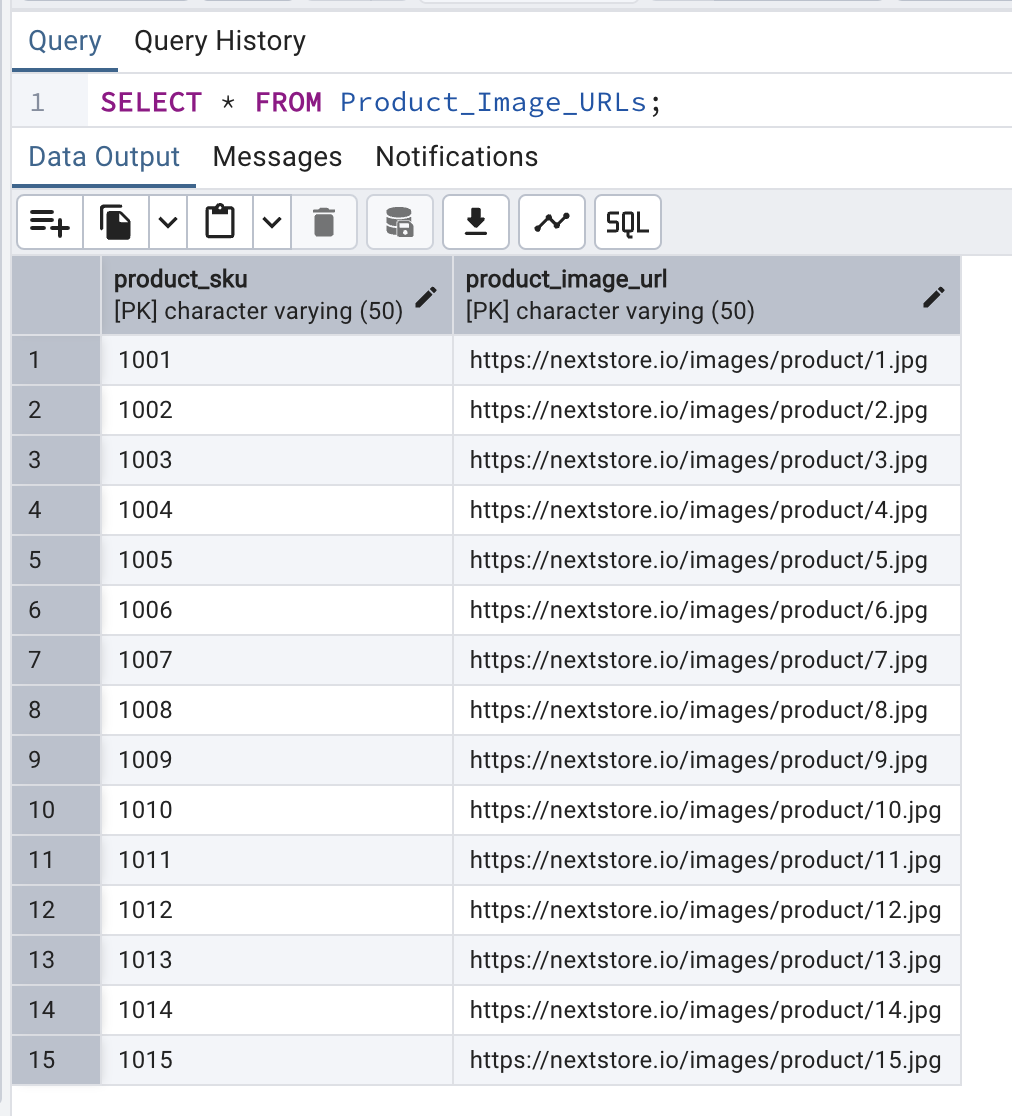
\includegraphics[width=1\textwidth]{images/sql/select/product_image_urls.png}
  \caption{\textit{Select from Product Image URLs Table}}
\end{figure}

\subsubsubsection{Review Image URLs}
The following script selects data from the Review Image URLs table.
\lstinputlisting[language=SQL, caption={\textit{Select from Review Image URLs Table}}]{sql/select/review_image_urls.sql}

\begin{figure}[H]
  \centering
  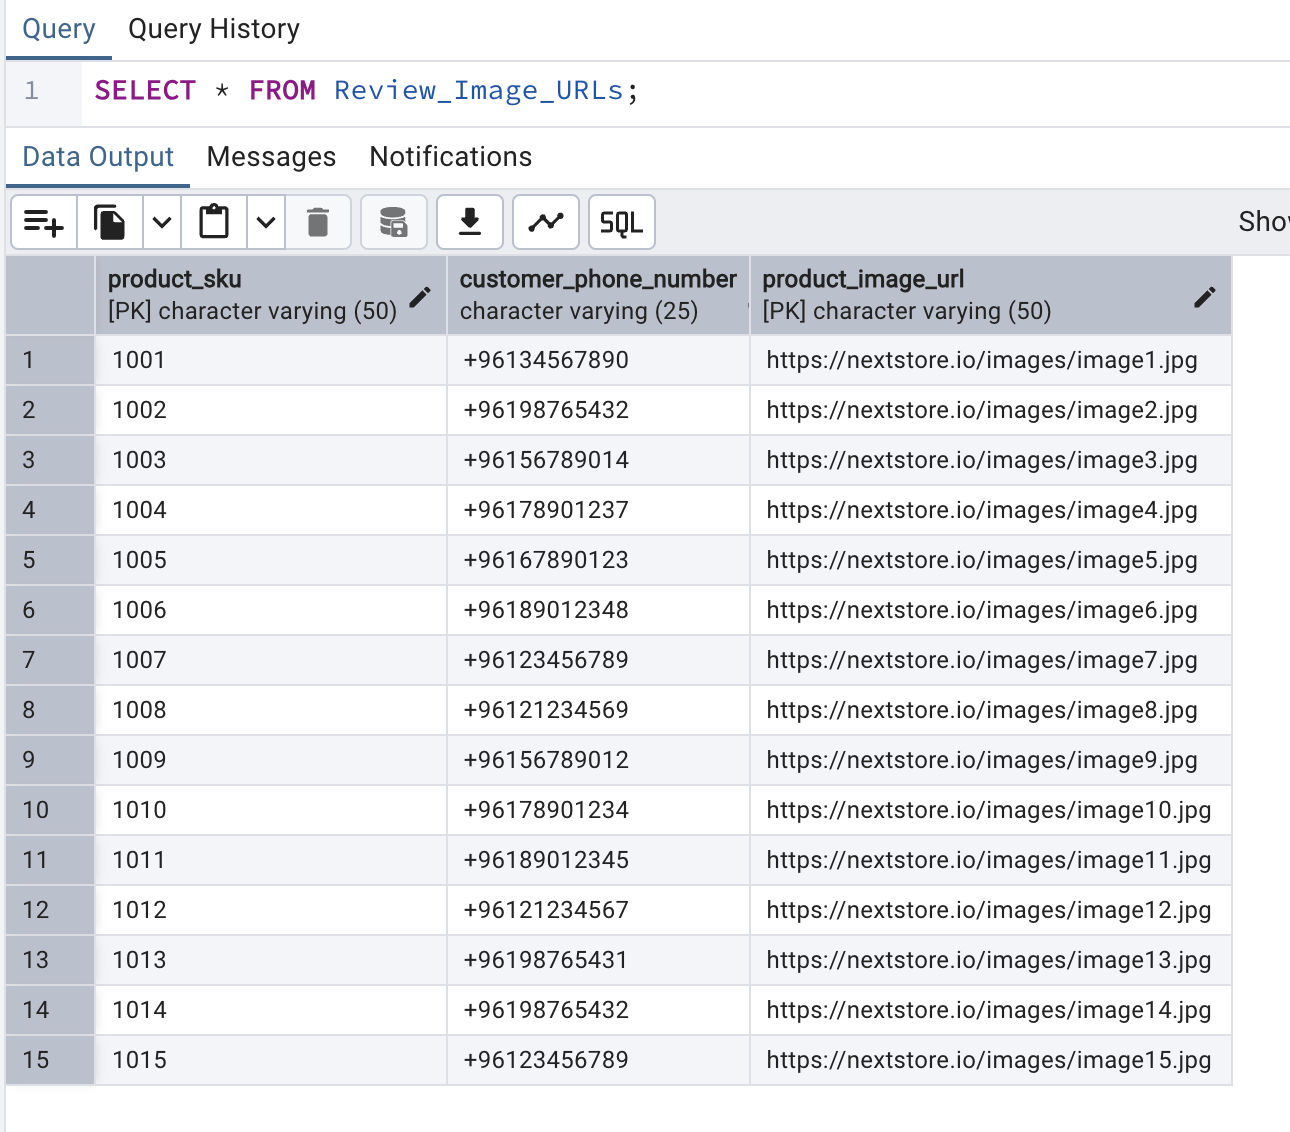
\includegraphics[width=1\textwidth]{images/sql/select/review_image_urls.png}
  \caption{\textit{Select from Review Image URLs Table}}
\end{figure}

\subsubsubsection{Located In}
The following script selects data from the Located In table.
\lstinputlisting[language=SQL, caption={\textit{Select from Located In Table}}]{sql/select/located_in.sql}

\begin{figure}[H]
  \centering
  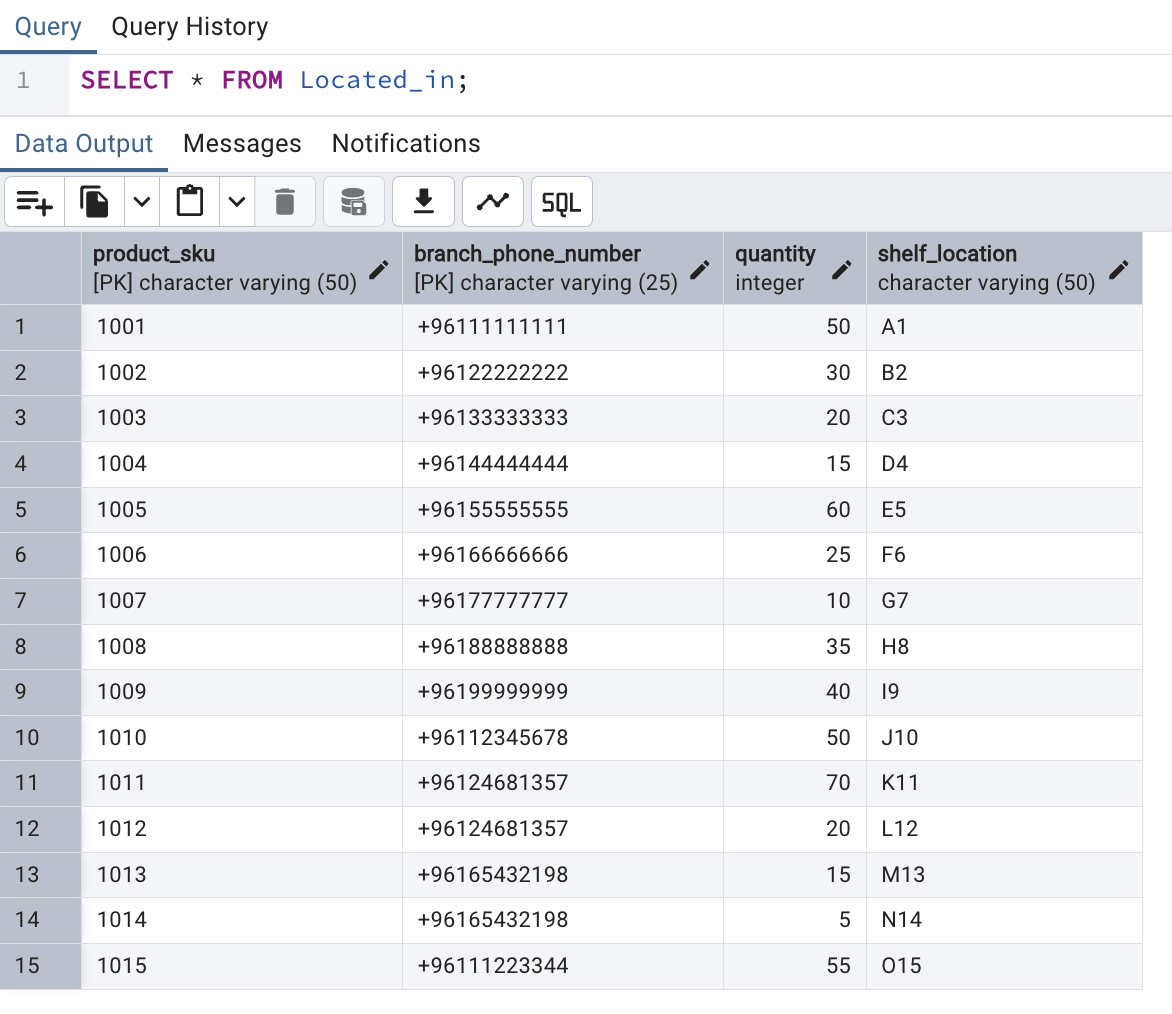
\includegraphics[width=1\textwidth]{images/sql/select/located_in.png}
  \caption{\textit{Select from Located In Table}}
\end{figure}

\subsubsubsection{Colors}
The following script selects data from the Colors table.
\lstinputlisting[language=SQL, caption={\textit{Select from Colors Table}}]{sql/select/colors.sql}

\begin{figure}[H]
  \centering
  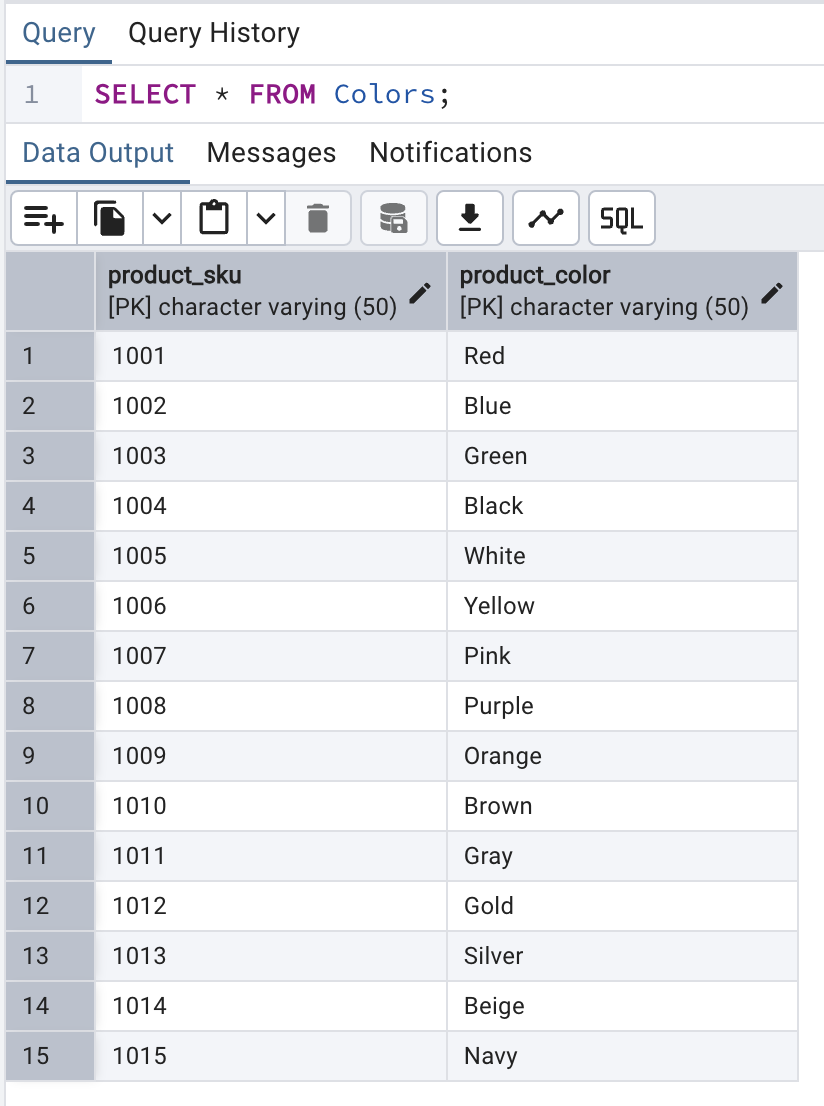
\includegraphics[width=1\textwidth]{images/sql/select/colors.png}
  \caption{\textit{Select from Colors Table}}
\end{figure}

\subsubsubsection{Coupon}
The following script selects data from the Coupon table.
\lstinputlisting[language=SQL, caption={\textit{Select from Coupon Table}}]{sql/select/coupon.sql}

\begin{figure}[H]
  \centering
  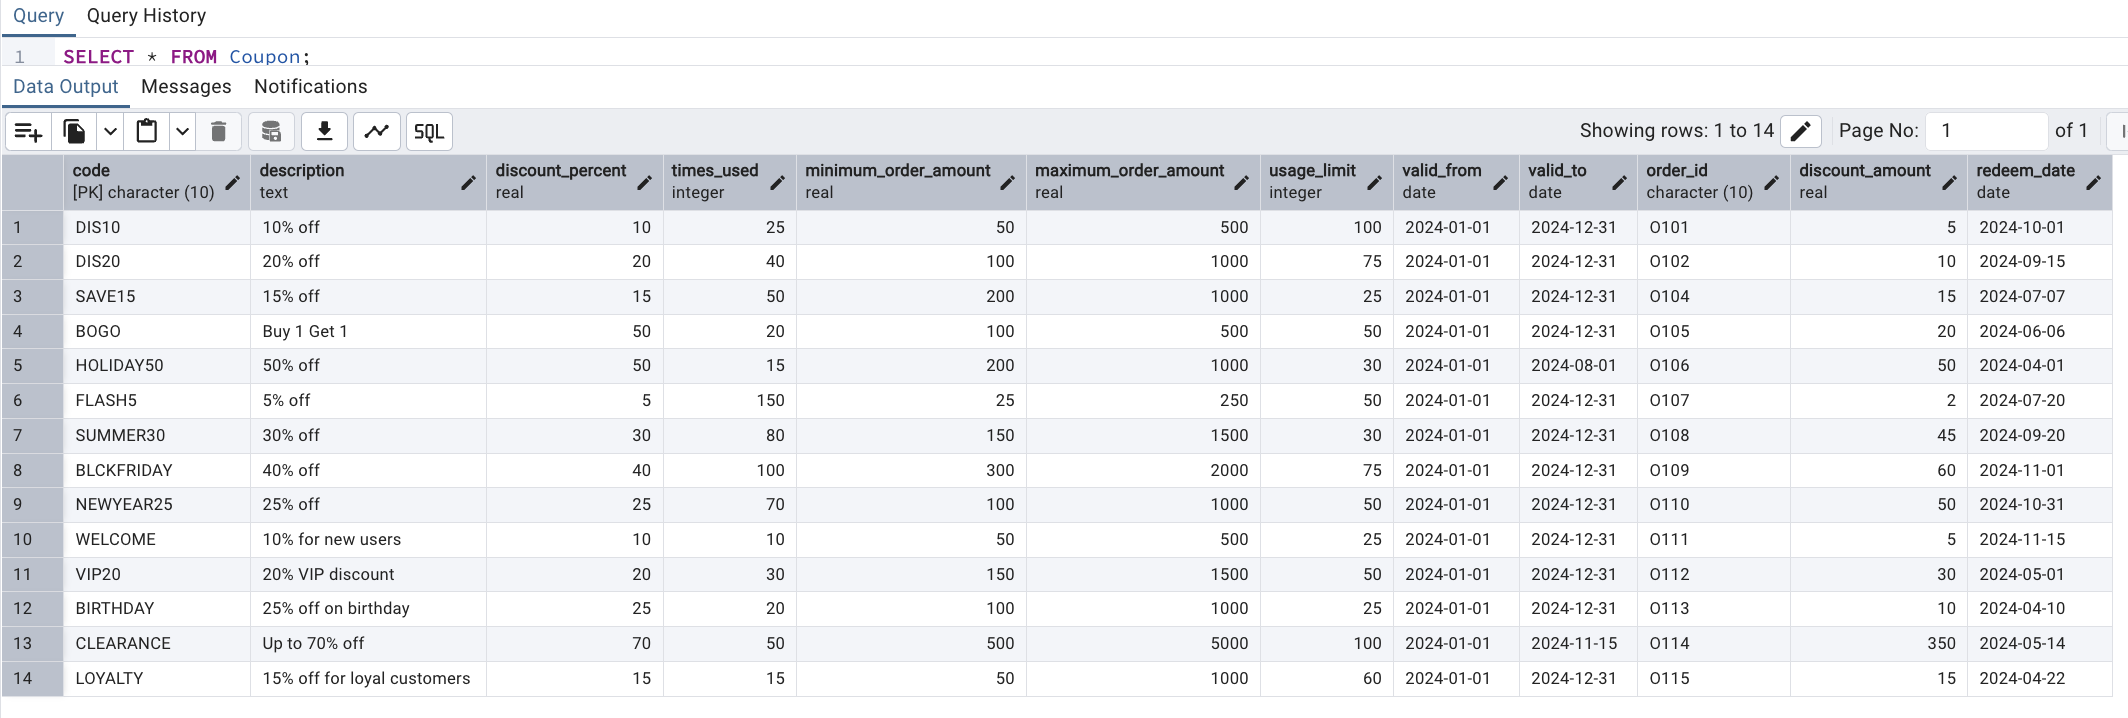
\includegraphics[width=1\textwidth]{images/sql/select/coupon.png}
  \caption{\textit{Select from Coupon Table}}
\end{figure}

\subsubsubsection{Department Location}
The following script selects data from the Department Location table.
\lstinputlisting[language=SQL, caption={\textit{Select from Department Location Table}}]{sql/select/department_location.sql}

\begin{figure}[H]
  \centering
  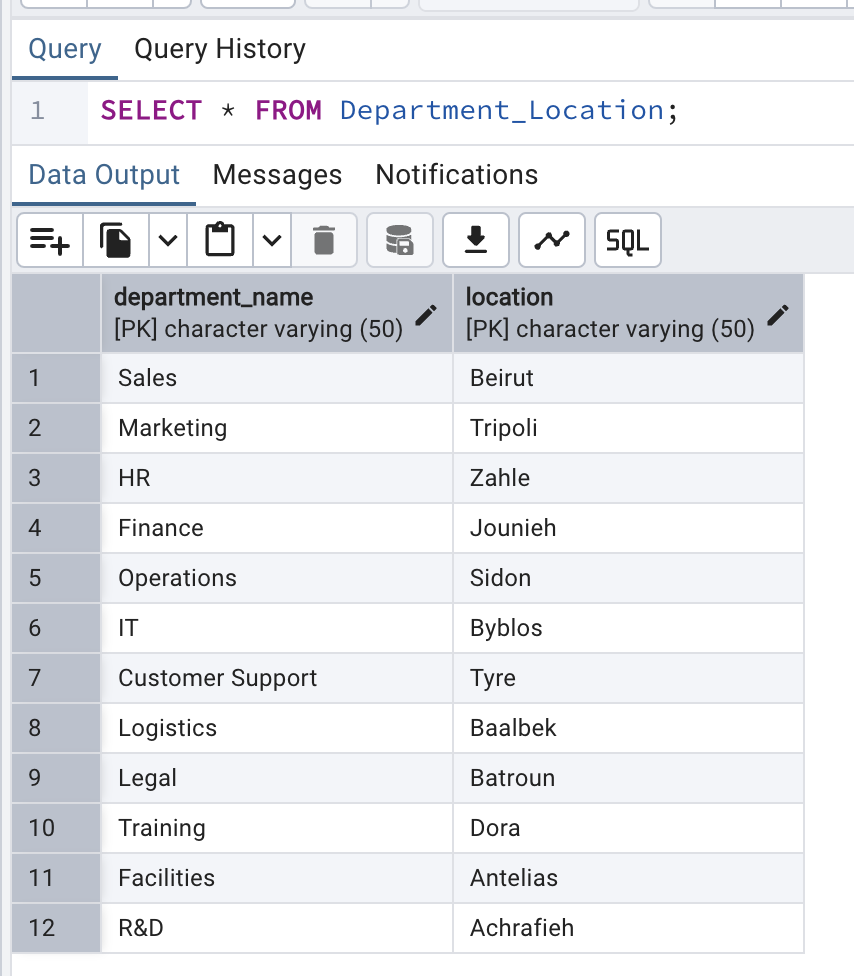
\includegraphics[width=1\textwidth]{images/sql/select/department_location.png}
  \caption{\textit{Select from Department Location Table}}
\end{figure}

\subsubsection{Complex Queries}

\subsubsubsection{Customer with Highest Number of Orders}

\lstinputlisting[language=SQL, caption={\textit{Customer with Highest Number of Orders}}]{sql/complex-queries/customer_with_highest_number_of_orders.sql}

\begin{figure}[H]
  \centering
  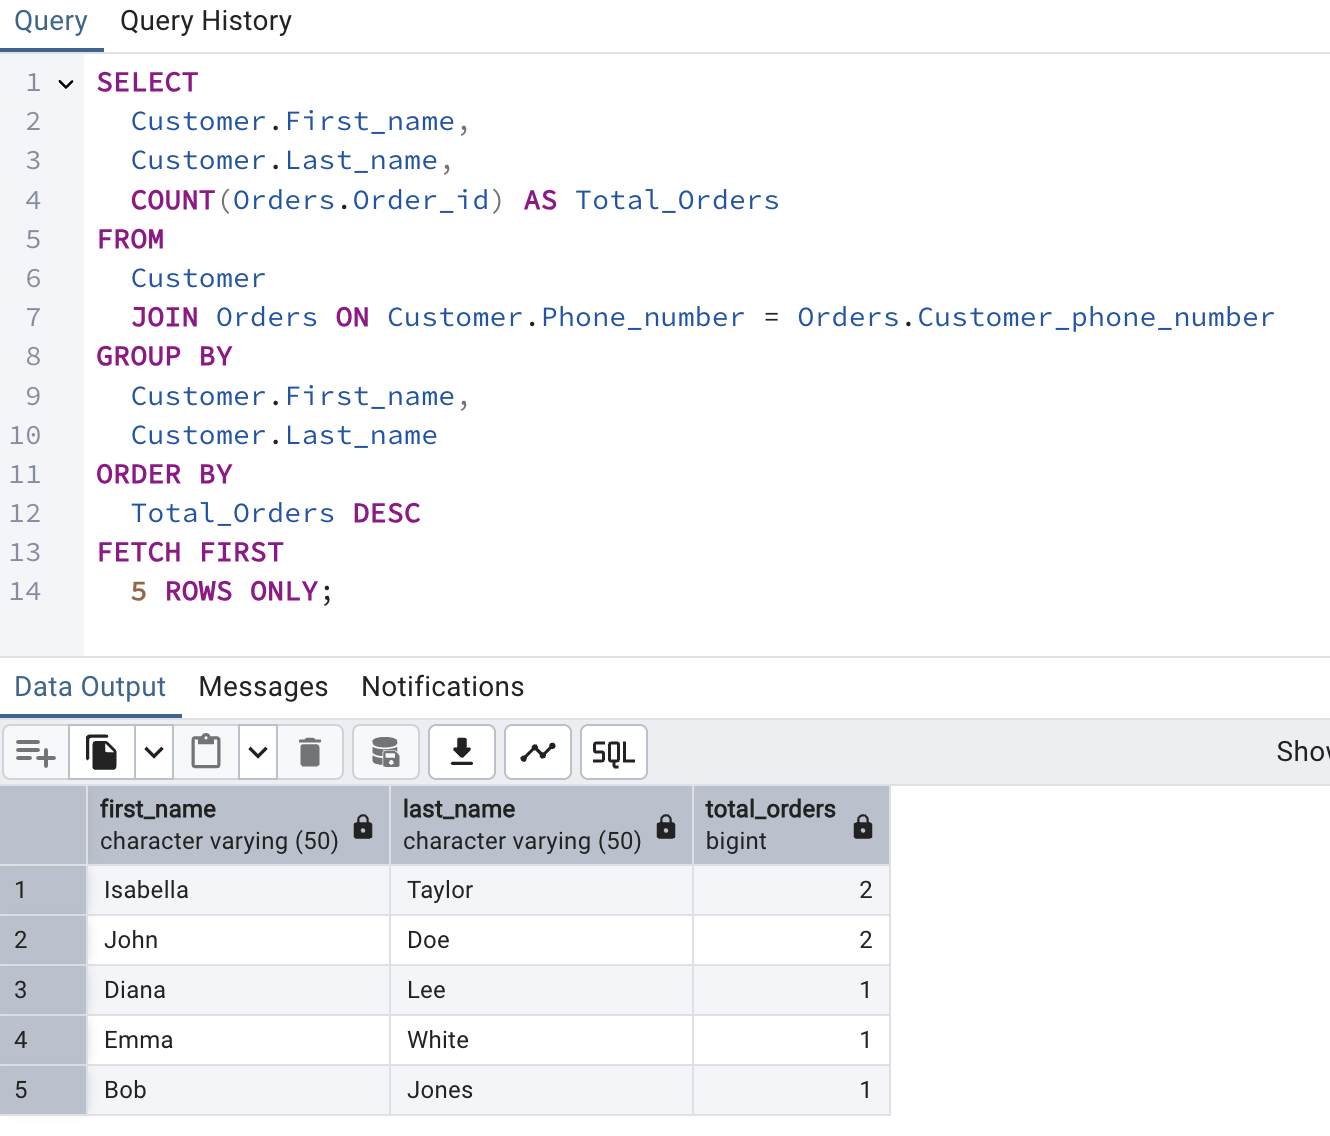
\includegraphics[width=1\textwidth]{images/sql/complex-queries/customer_with_highest_number_of_orders.png}
  \caption{\textit{Customer with Highest Number of Orders}}
\end{figure}

This SQL query retrieves the top 5 customers who have placed the highest number of orders. It joins the Customer and Order tables on the Phone\_number and Customer\_phone\_number fields, respectively. The query groups the results by the customers' first and last names, counts the number of orders for each customer, and orders the results in descending order based on the total number of orders. Finally, it limits the output to the top 5 customers. This query is useful for identifying the most active customers, which can help in targeting marketing efforts, improving customer service, and understanding customer behavior.

\subsubsubsection{Products with Highest Revenue}

\lstinputlisting[language=SQL, caption={\textit{Products with Highest Revenue}}]{sql/complex-queries/products_with_highest_revenue.sql}

\begin{figure}[H]
  \centering
  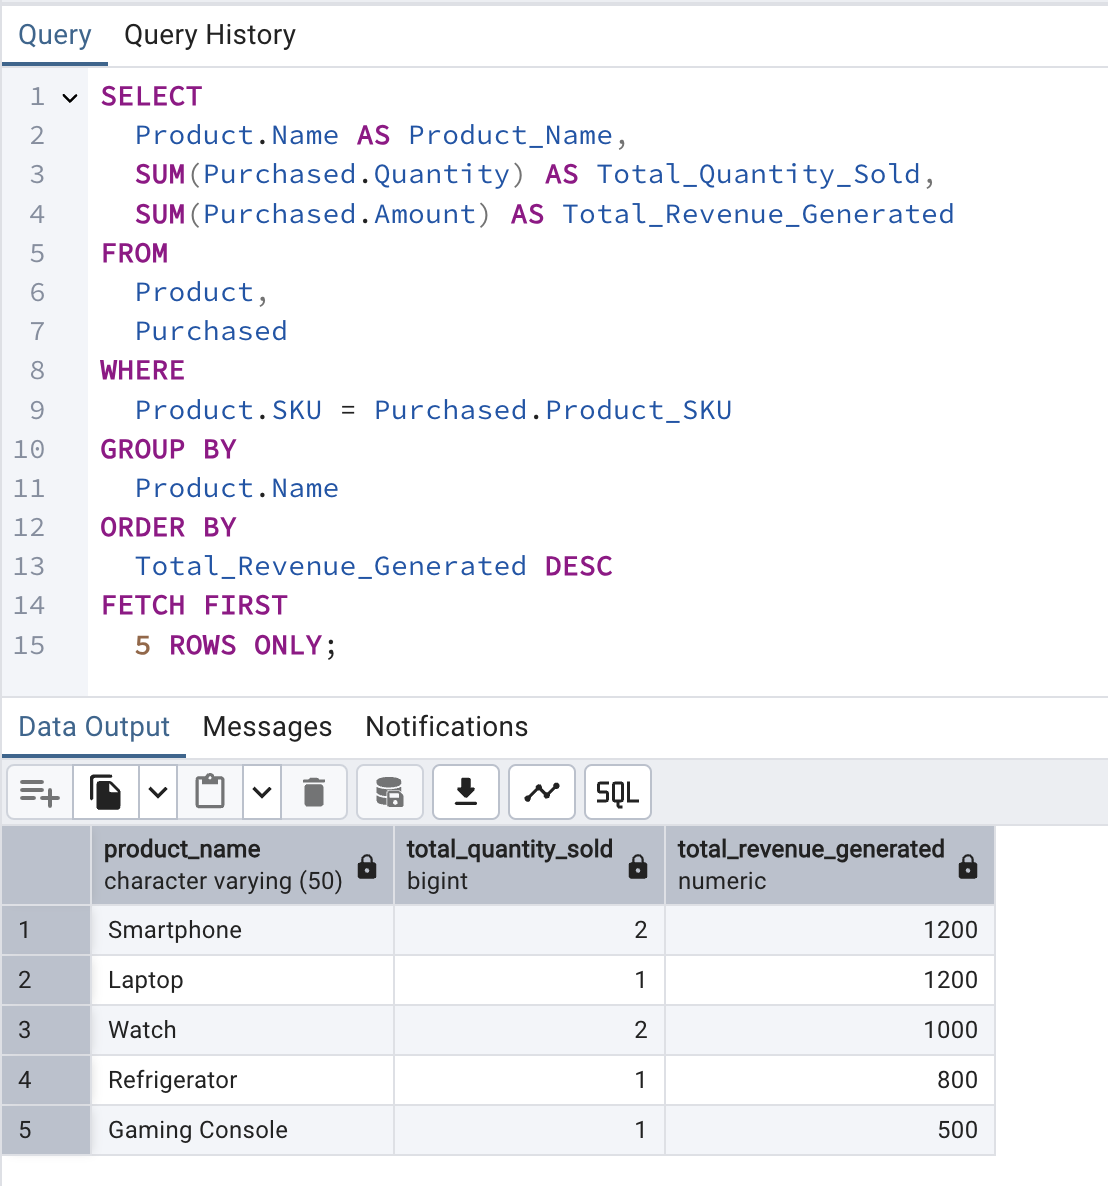
\includegraphics[width=1\textwidth]{images/sql/complex-queries/products_with_highest_revenue.png}
  \caption{\textit{Products with Highest Revenue}}
\end{figure}

This SQL query retrieves the top 5 products that have generated the highest revenue. It selects the product name, the total quantity sold, and the total revenue generated for each product. The query joins the Product and Purchased tables on the SKU and Product\_SKU columns, respectively. It then groups the results by product name and orders them by total revenue in descending order. Finally, it limits the results to the top 5 rows. This is useful for businesses to identify their best-selling products and make informed decisions about inventory, marketing, and sales strategies.

\subsubsubsection{Most Sold Product in Each Branch}

\lstinputlisting[language=SQL, caption={\textit{Most Sold Product in Each Branch}}]{sql/complex-queries/most_sold_product_in_each_branch.sql}

\begin{figure}[H]
  \centering
  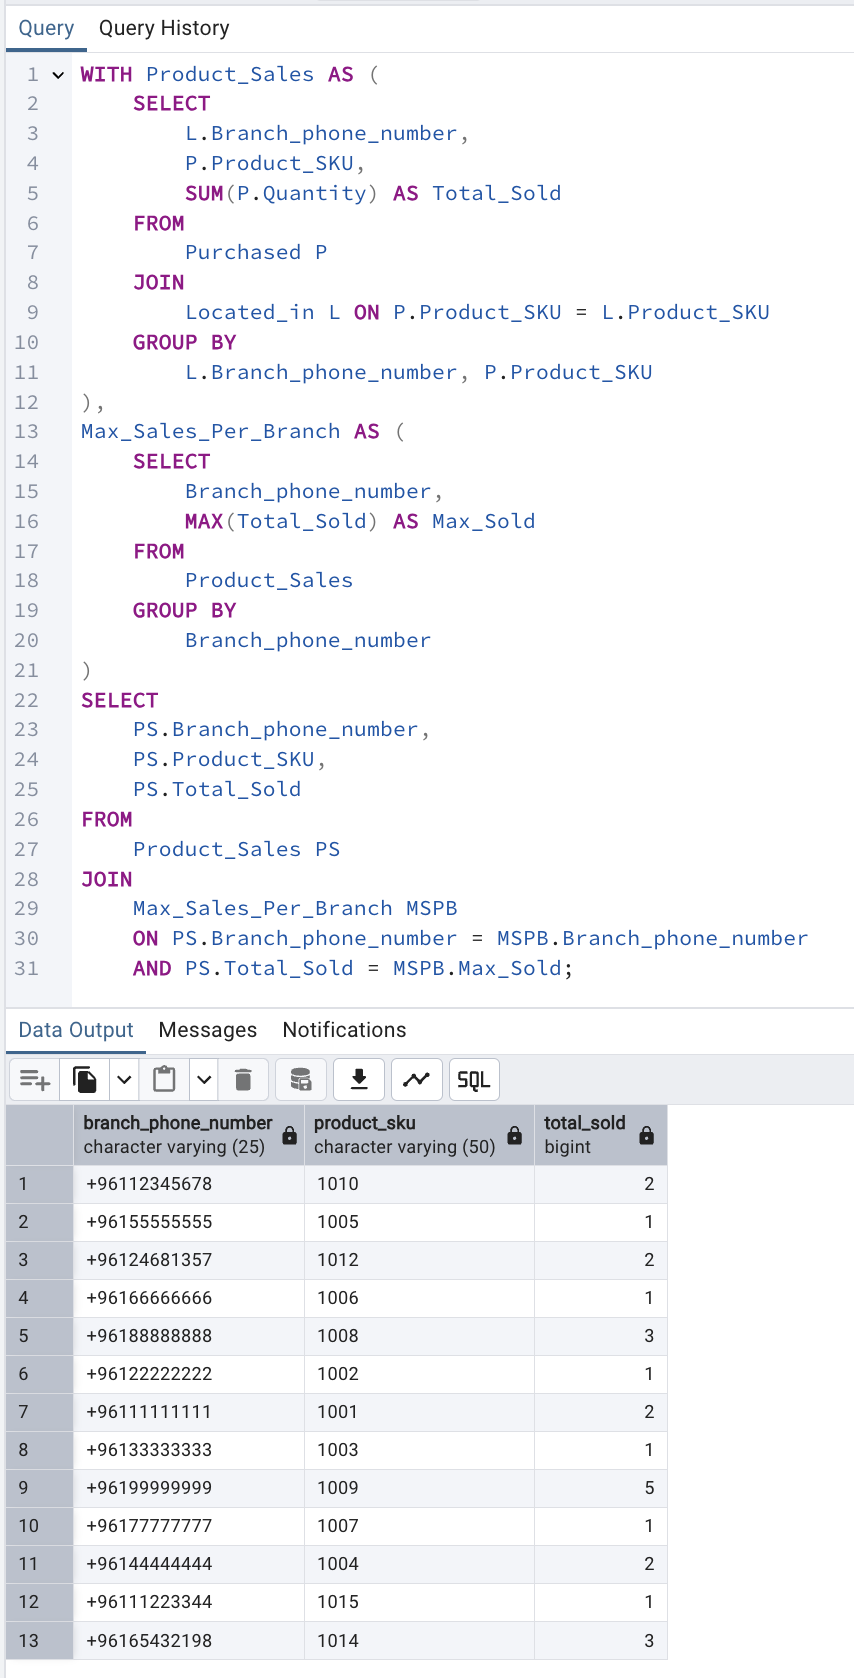
\includegraphics[width=0.7\textwidth]{images/sql/complex-queries/most_sold_product_in_each_branch.png}
  \caption{\textit{Most Sold Product in Each Branch}}
\end{figure}

This SQL query identifies the most sold product in each branch by calculating the total quantity sold for each product at each branch. It first joins the Purchased and Located\_in tables on the Product\_SKU field. Then, it groups the results by branch phone number and product SKU, summing the quantities sold. The HAVING clause filters these groups to only include the product with the maximum total quantity sold per branch. This is useful for businesses to understand which products are the top sellers at each branch, enabling better inventory management and targeted marketing strategies.

\subsubsubsection{Calculate Customer Lifetime Value for Each Customer}

\lstinputlisting[language=SQL, caption={\textit{Calculate Customer Lifetime Value for Each Customer}}]{sql/complex-queries/calculate_customer_lifetime_value.sql}

\begin{figure}[H]
  \centering
  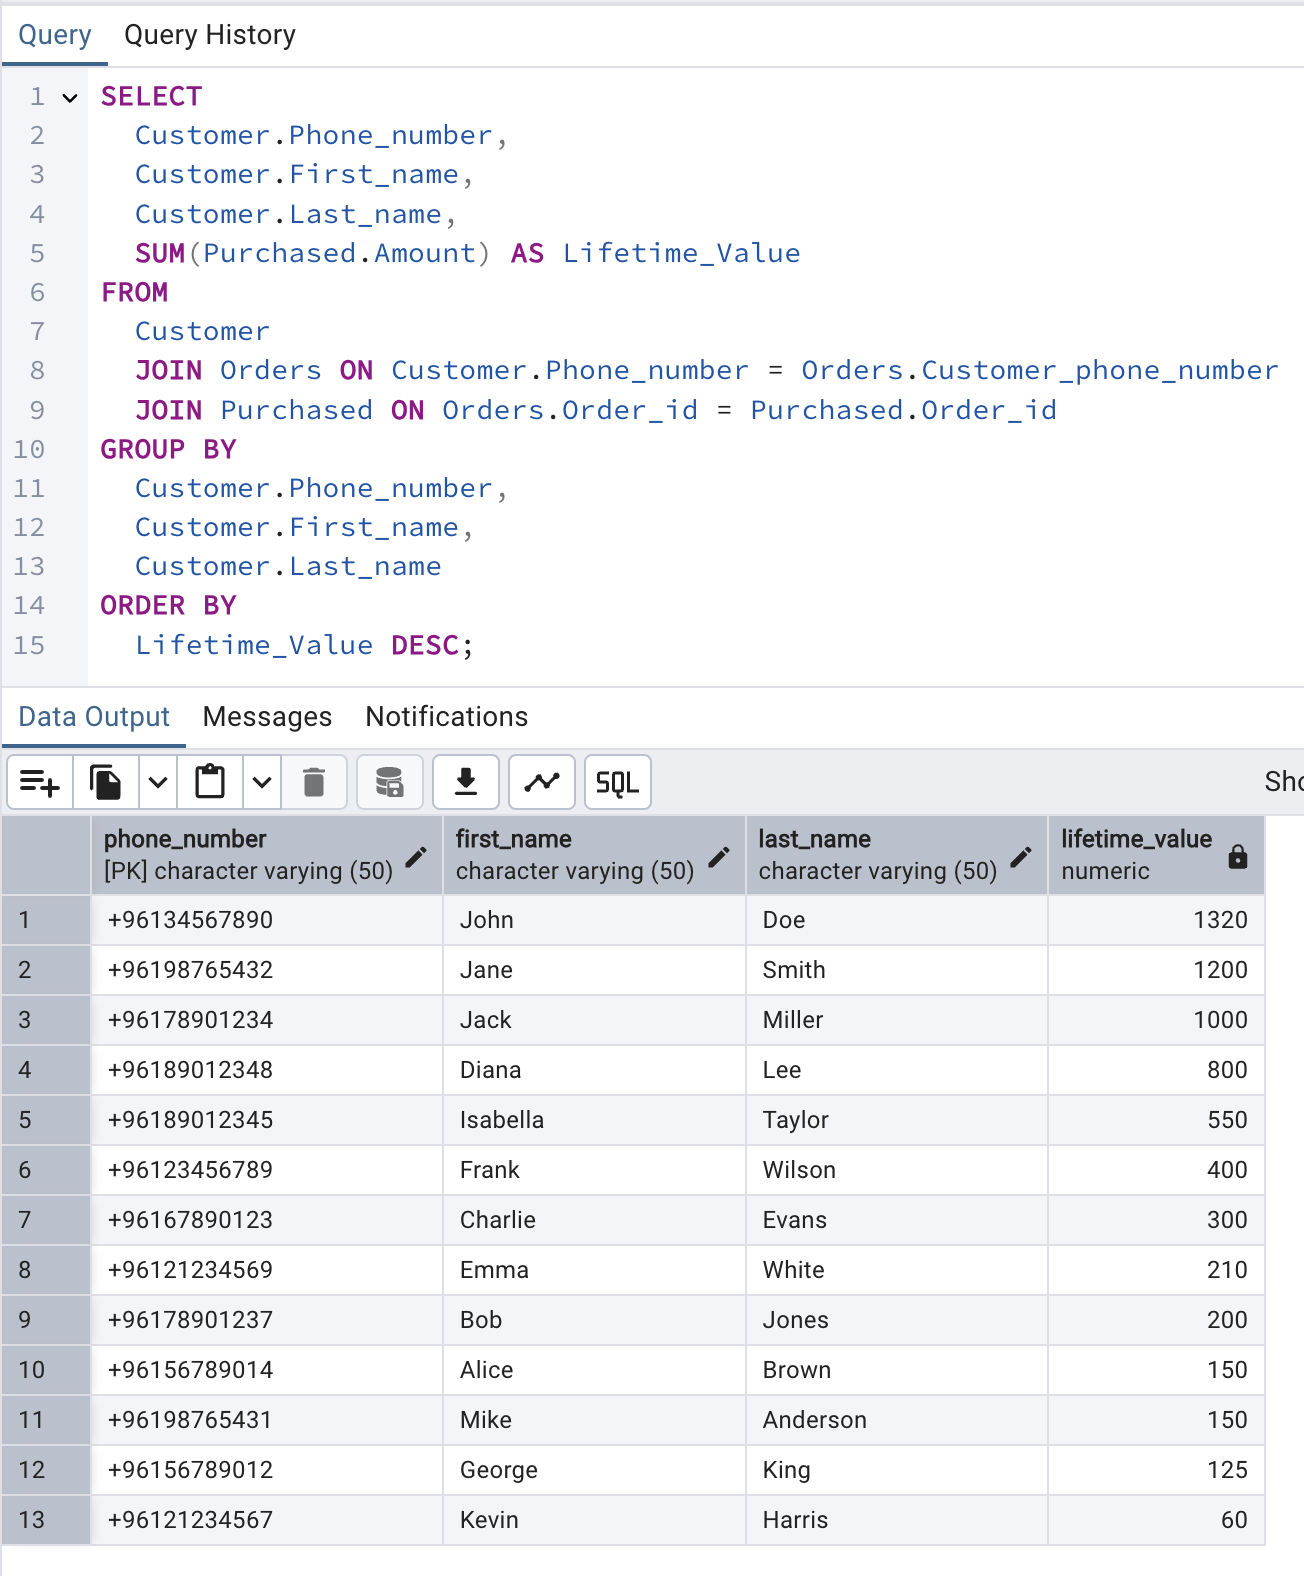
\includegraphics[width=1\textwidth]{images/sql/complex-queries/calculate_customer_lifetime_value.png}
  \caption{\textit{Calculate Customer Lifetime Value for Each Customer}}
\end{figure}

This SQL query calculates the Customer Lifetime Value for each customer by summing up the total amount spent by each customer across all their orders. It joins three tables: Customer, Orders, and Purchased, using the customer's phone number and order ID to link the data. The results are grouped by the customer's phone number, first name, and last name, and then ordered by the lifetime value in descending order. This is useful for businesses to identify their most valuable customers, enabling them to tailor marketing strategies, improve customer retention, and allocate resources more effectively.

\subsubsubsection{Underperforming Products}

\lstinputlisting[language=SQL, caption={\textit{Underperforming Products}}]{sql/complex-queries/underperforming_products.sql}

\begin{figure}[H]
  \centering
  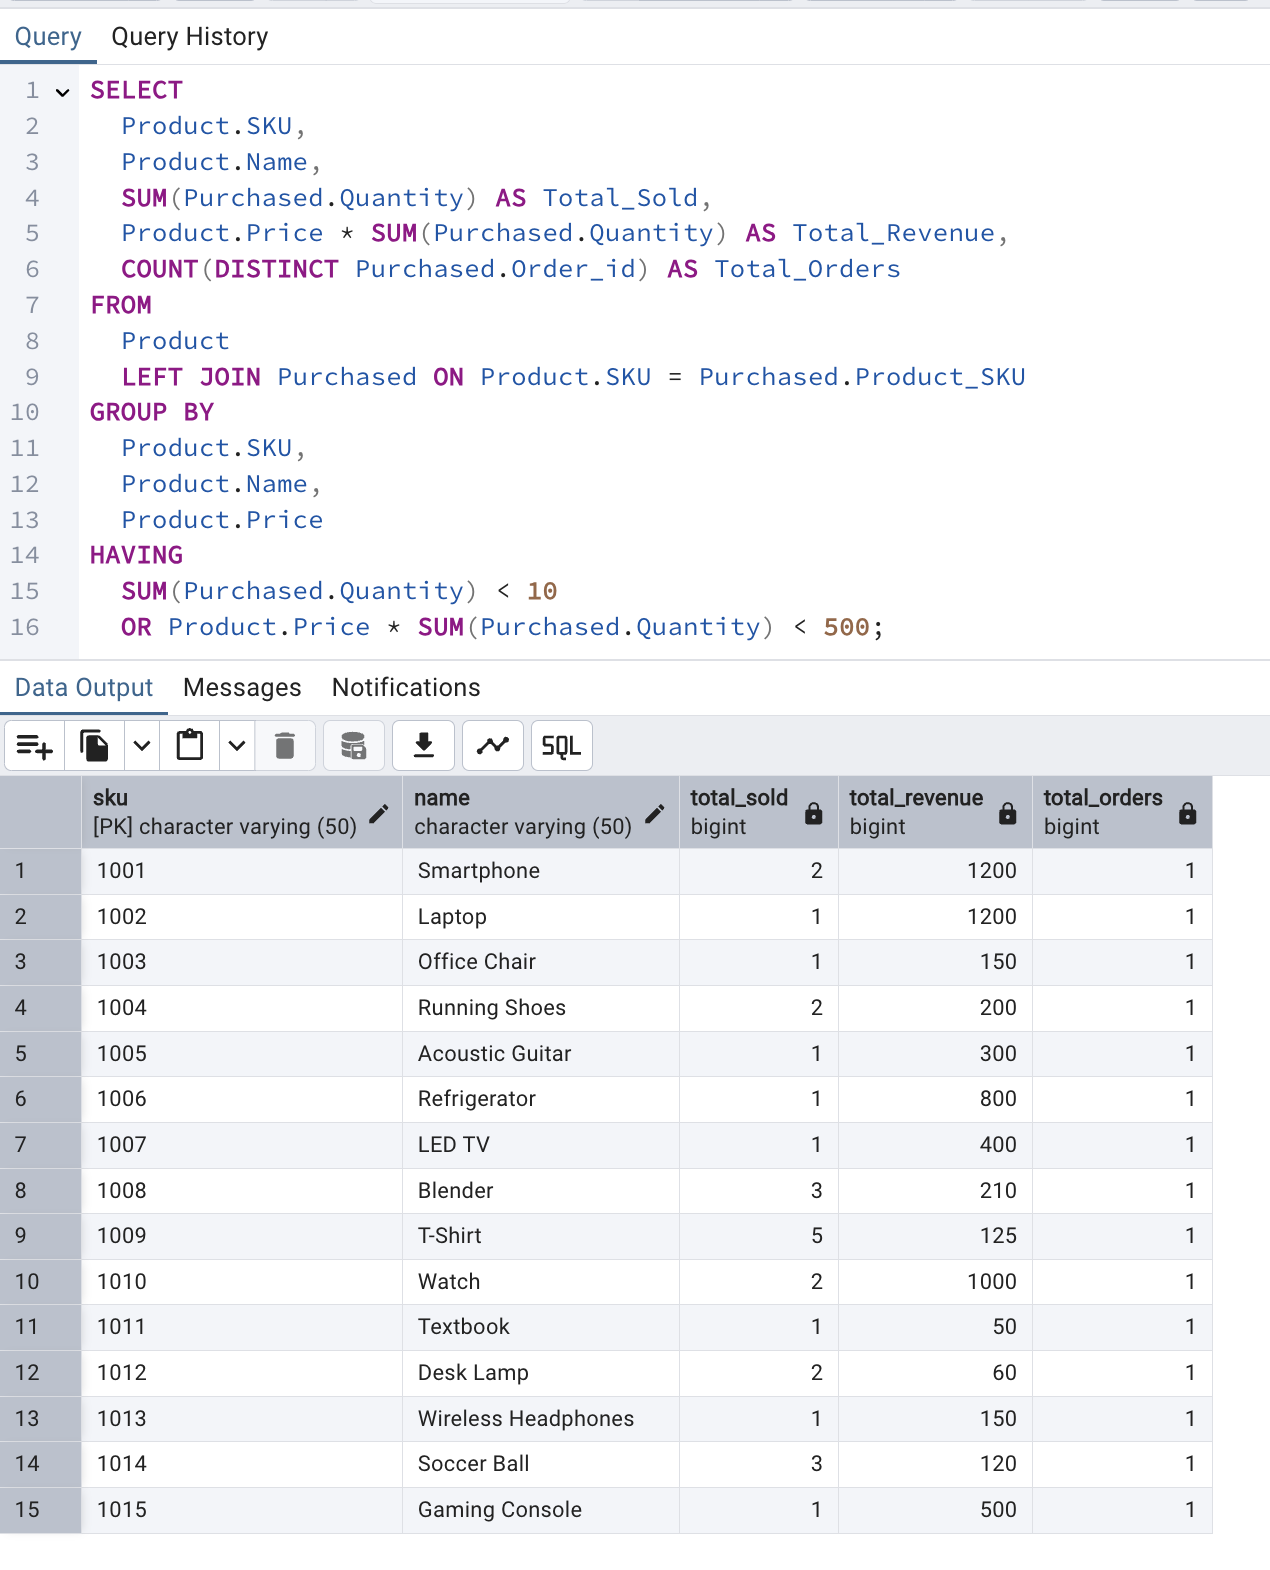
\includegraphics[width=1\textwidth]{images/sql/complex-queries/underperforming_products.png}
  \caption{\textit{Underperforming Products}}
\end{figure}

This SQL query identifies underperforming products by selecting products that have either sold fewer than 10 units or generated less than \$500 in total revenue. It joins the Product table with the Purchased table on the SKU field to aggregate sales data. The query calculates the total quantity sold (Total\_Sold), total revenue (Total\_Revenue), and the number of distinct orders (Total\_Orders) for each product. The HAVING clause filters the results to include only those products that meet the underperformance criteria. This is useful for businesses to identify products that may need marketing attention, discounts, or discontinuation.

\subsubsubsection{Find Popular Products Combinations}

\lstinputlisting[language=SQL, caption={\textit{Find Popular Products Combinations}}]{sql/complex-queries/find_popular_products_combinations.sql}

\begin{figure}[H]
  \centering
  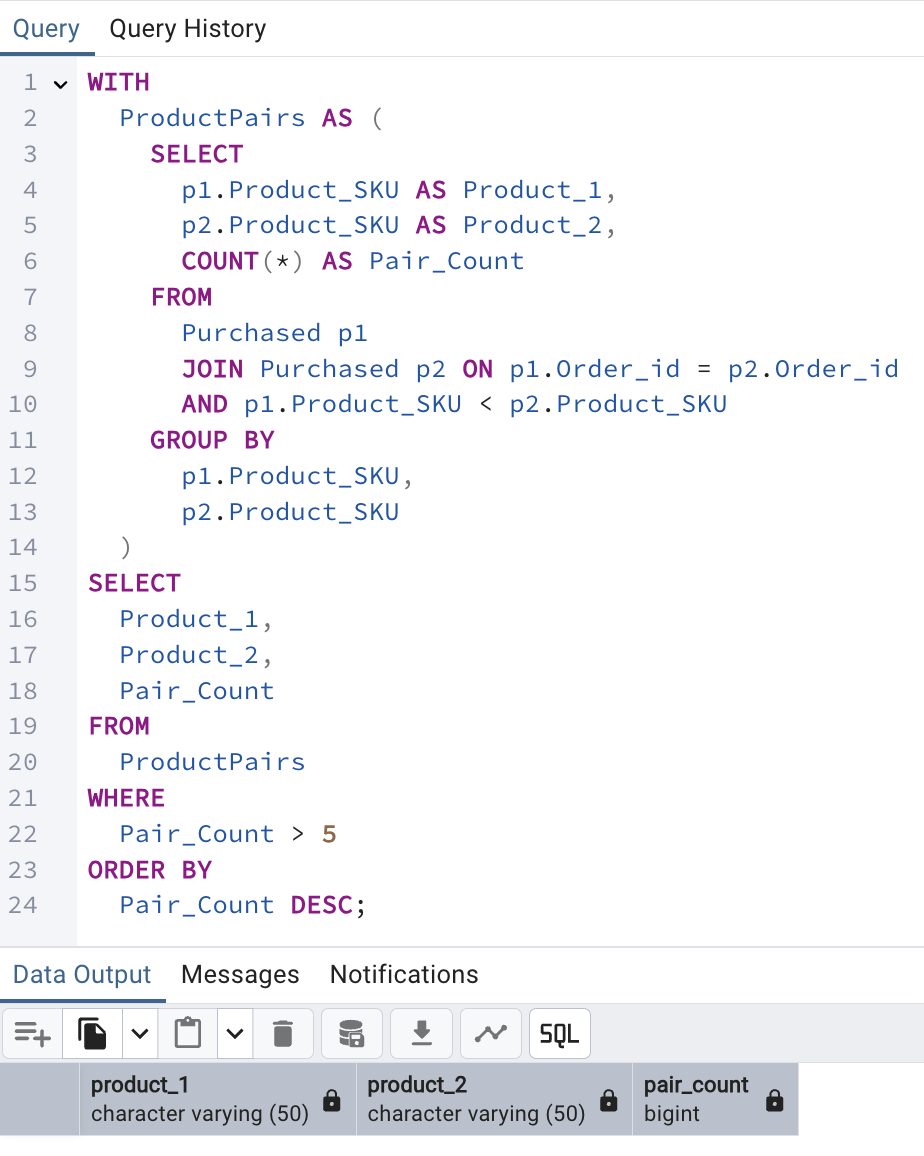
\includegraphics[width=1\textwidth]{images/sql/complex-queries/find_popular_products_combinations.png}
  \caption{\textit{Find Popular Products Combinations}}
\end{figure}

This SQL query identifies popular product combinations that are frequently purchased together. It uses a Common Table Expression (CTE) named ProductPairs to join the Purchased table with itself, matching rows where the Order\_id is the same but the Product\_SKU is different. The condition p1.Product\_SKU < p2.Product\_SKU ensures that each pair is counted only once. The query then groups these pairs and counts how often each combination appears. Finally, it selects pairs that appear more than five times and orders them by their frequency in descending order. This information is useful for understanding customer purchasing behavior, which can inform marketing strategies, product placement, and inventory management.

\subsubsubsection{Products with the Most Discounts}

\lstinputlisting[language=SQL, caption={\textit{Products with the Most Discounts}}]{sql/complex-queries/products_with_the_most_discounts.sql}

\begin{figure}[H]
  \centering
  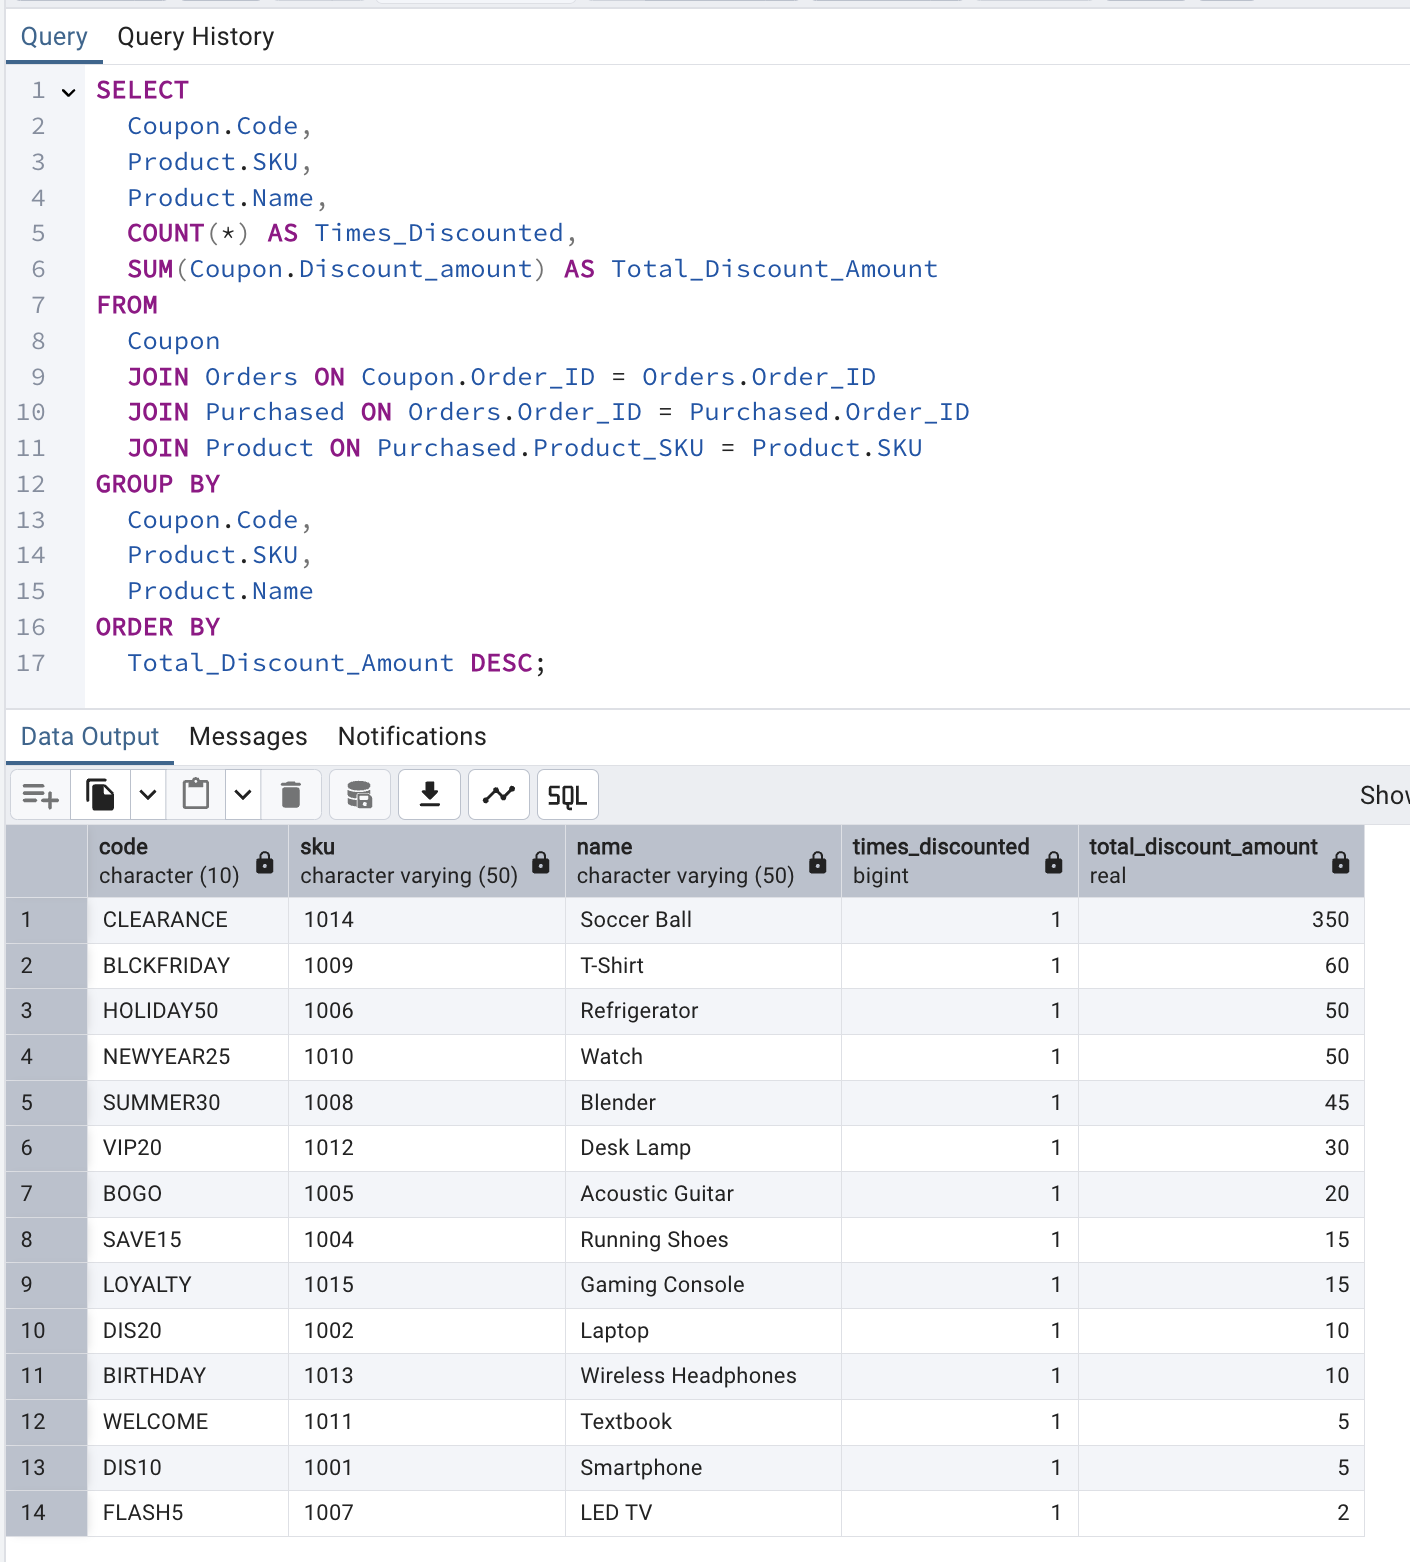
\includegraphics[width=1\textwidth]{images/sql/complex-queries/products_with_the_most_discounts.png}
  \caption{\textit{Products with the Most Discounts}}
\end{figure}

This SQL query retrieves and aggregates data about discounts applied to products. It joins four tables: Coupon, Orders, Purchased, and Product. The query selects the coupon code, product SKU, product name, the count of times each coupon was used (Times\_Discounted), and the total discount amount for each product (Total\_Discount\_Amount). The results are grouped by coupon code, product SKU, and product name, and then ordered by the total discount amount in descending order. This is useful for analyzing the effectiveness of different coupons and understanding which products benefit most from discounts, aiding in marketing and sales strategy decisions.

\subsubsubsection{Seasonal Trends for Product Categories}

\lstinputlisting[language=SQL, caption={\textit{Seasonal Trends for Product Categories}}]{sql/complex-queries/seasonal_trends_for_product_categories.sql}

\begin{figure}[H]
  \centering
  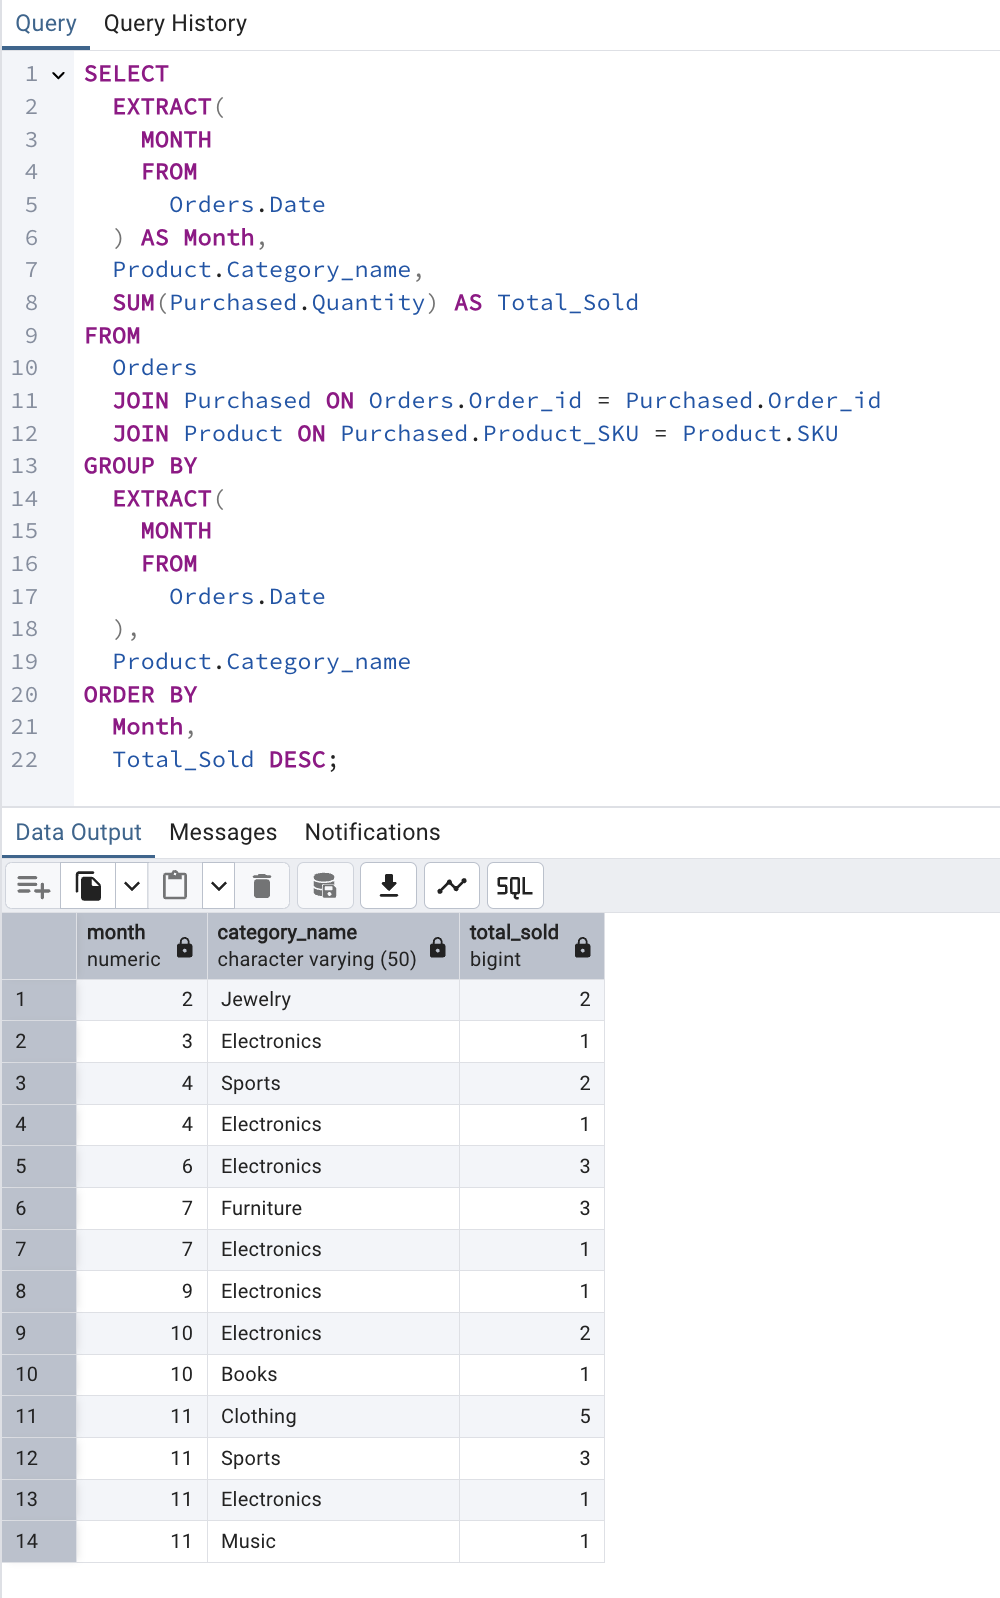
\includegraphics[width=0.7\textwidth]{images/sql/complex-queries/seasonal_trends_for_product_categories.png}
  \caption{\textit{Seasonal Trends for Product Categories}}
\end{figure}

This SQL query is designed to analyze seasonal trends in product categories by aggregating sales data on a monthly basis. It extracts the month from the Orders.Date field and groups the results by both the month and the product category name. The query then sums the quantity of products sold (Purchased.Quantity) for each category within each month. The results are ordered first by month and then by the total quantity sold in descending order. This analysis is useful for identifying which product categories perform best during different times of the year, enabling businesses to make informed decisions about inventory management, marketing strategies, and sales forecasting.

\subsubsubsection{Branches with Stock Shortages}

\lstinputlisting[language=SQL, caption={\textit{Branches with Stock Shortages}}]{sql/complex-queries/branches_with_stock_shortages.sql}

\begin{figure}[H]
  \centering
  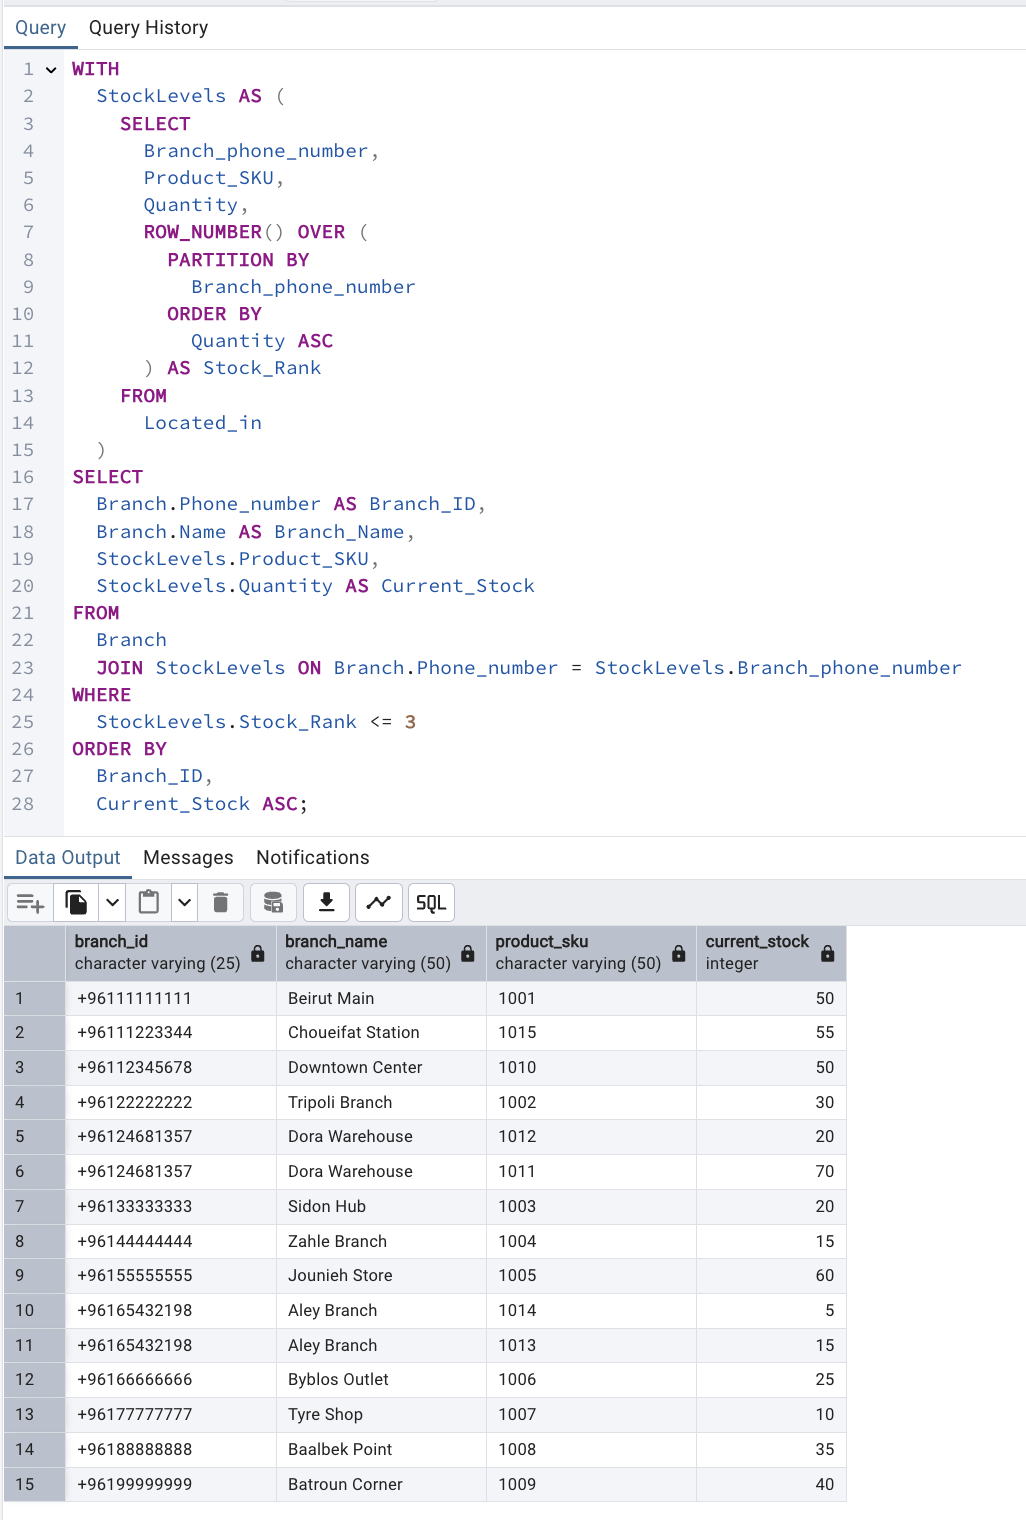
\includegraphics[width=1\textwidth]{images/sql/complex-queries/branches_with_stock_shortages.png}
  \caption{\textit{Branches with Stock Shortages}}
\end{figure}

This SQL query identifies branches with stock shortages by ranking products based on their quantity at each branch. The StockLevels Common Table Expression (CTE) calculates the rank of each product's stock quantity within each branch using the ROW\_NUMBER() function. The main query then selects branches and their products where the stock quantity ranks in the lowest three (Stock\_Rank <= 3). This information is useful for the company to quickly identify and address potential stock shortages, ensuring that branches are adequately stocked and can meet customer demand, thereby improving inventory management and operational efficiency.

\subsubsubsection{Best Performing Branch}

\lstinputlisting[language=SQL, caption={\textit{Best Performing Branch}}]{sql/complex-queries/best_performing_branch.sql}

\begin{figure}[H]
  \centering
  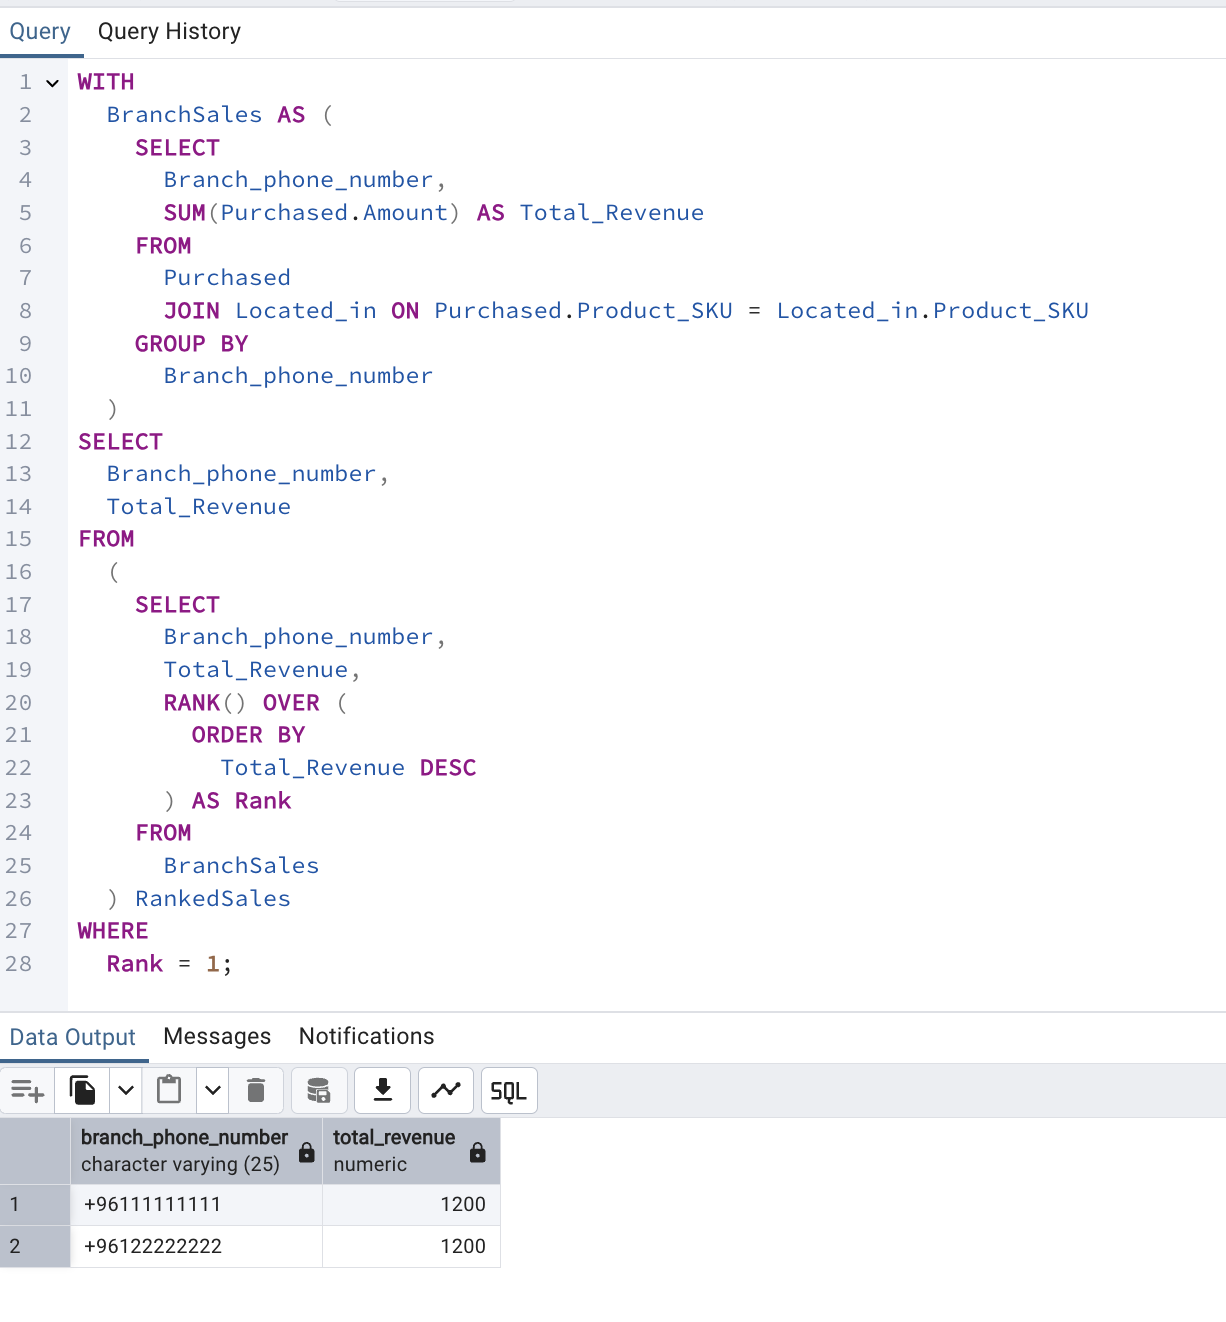
\includegraphics[width=1\textwidth]{images/sql/complex-queries/best_performing_branch.png}
  \caption{\textit{Best Performing Branch}}
\end{figure}

This SQL query identifies the best-performing branch based on total revenue from sales. It first calculates the total revenue for each branch by summing the amounts from the Purchased table, joined with the Located\_in table to associate products with branches. The results are grouped by branch phone number. Then, it ranks these branches by total revenue in descending order. Finally, it selects the branch with the highest total revenue (ranked 1). This information is useful for the company as it highlights the most successful branch, allowing management to analyze and replicate its strategies across other branches to improve overall performance.

\subsection{Views}

\subsubsection{Customer orders}

\lstinputlisting[language=SQL, caption={\textit{Customer Orders View}}]{sql/views/customer_orders.sql}

\begin{figure}[H]
  \centering
  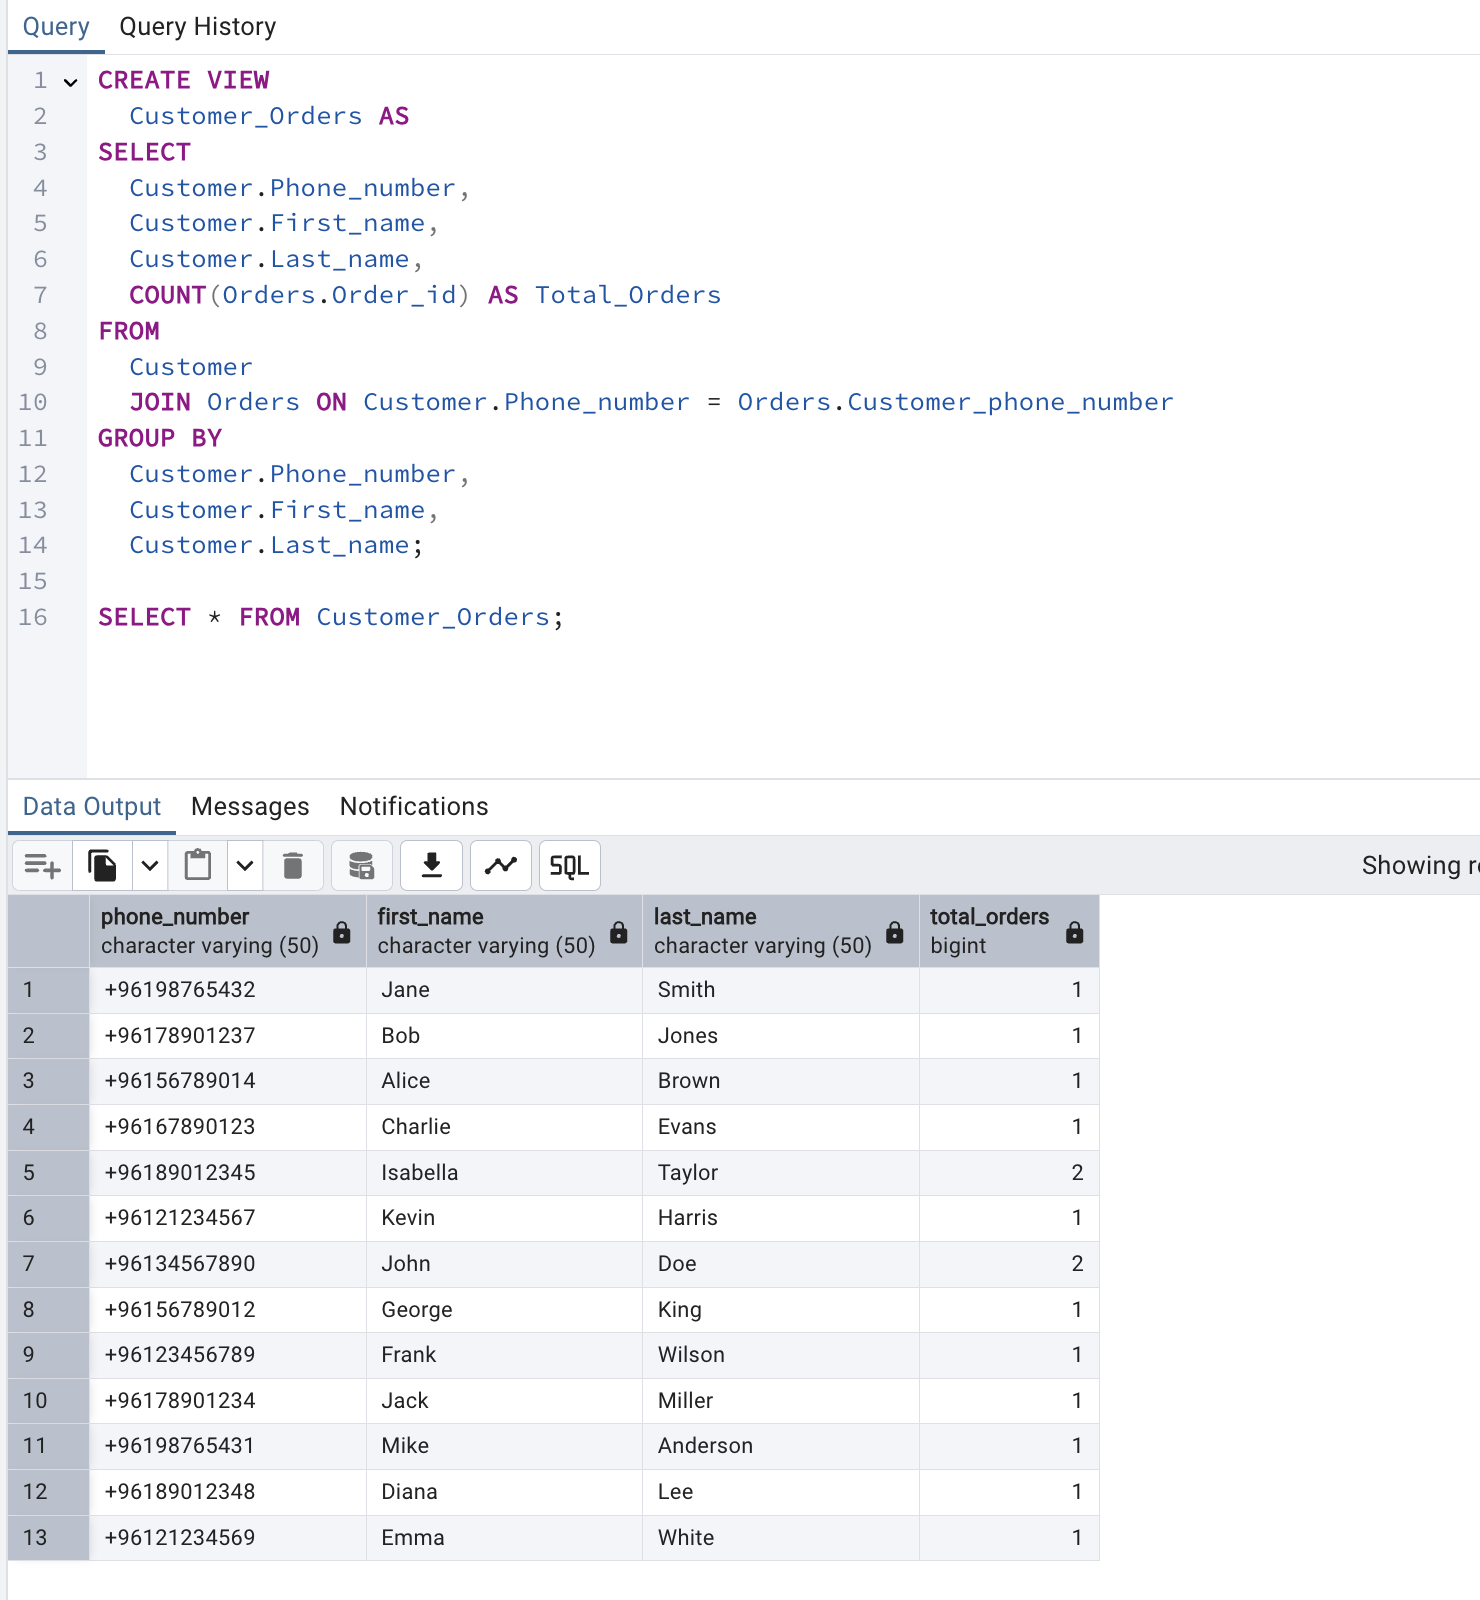
\includegraphics[width=1\textwidth]{images/sql/views/customer_orders.png}
  \caption{\textit{Customer Orders View}}
\end{figure}

Creating the Customer\_Orders view is essential for simplifying and organizing data retrieval related to customer orders. This view consolidates information from the Customer and Order tables, providing a clear and concise summary of each customer's total orders. By joining these tables on the customer's phone number and grouping the results by customer details, the view enables efficient querying and reporting without repeatedly writing complex SQL joins and aggregations. This enhances readability, maintainability, and performance of database operations, making it easier for analysts and developers to access and analyze customer order data.

\subsubsection{Update of the number of employees in the Department}

\lstinputlisting[language=SQL, caption={\textit{Update of the Number of Employees in the Department View}}]{sql/views/update_number_of_employees_in_department.sql}

\begin{figure}[H]
  \centering
  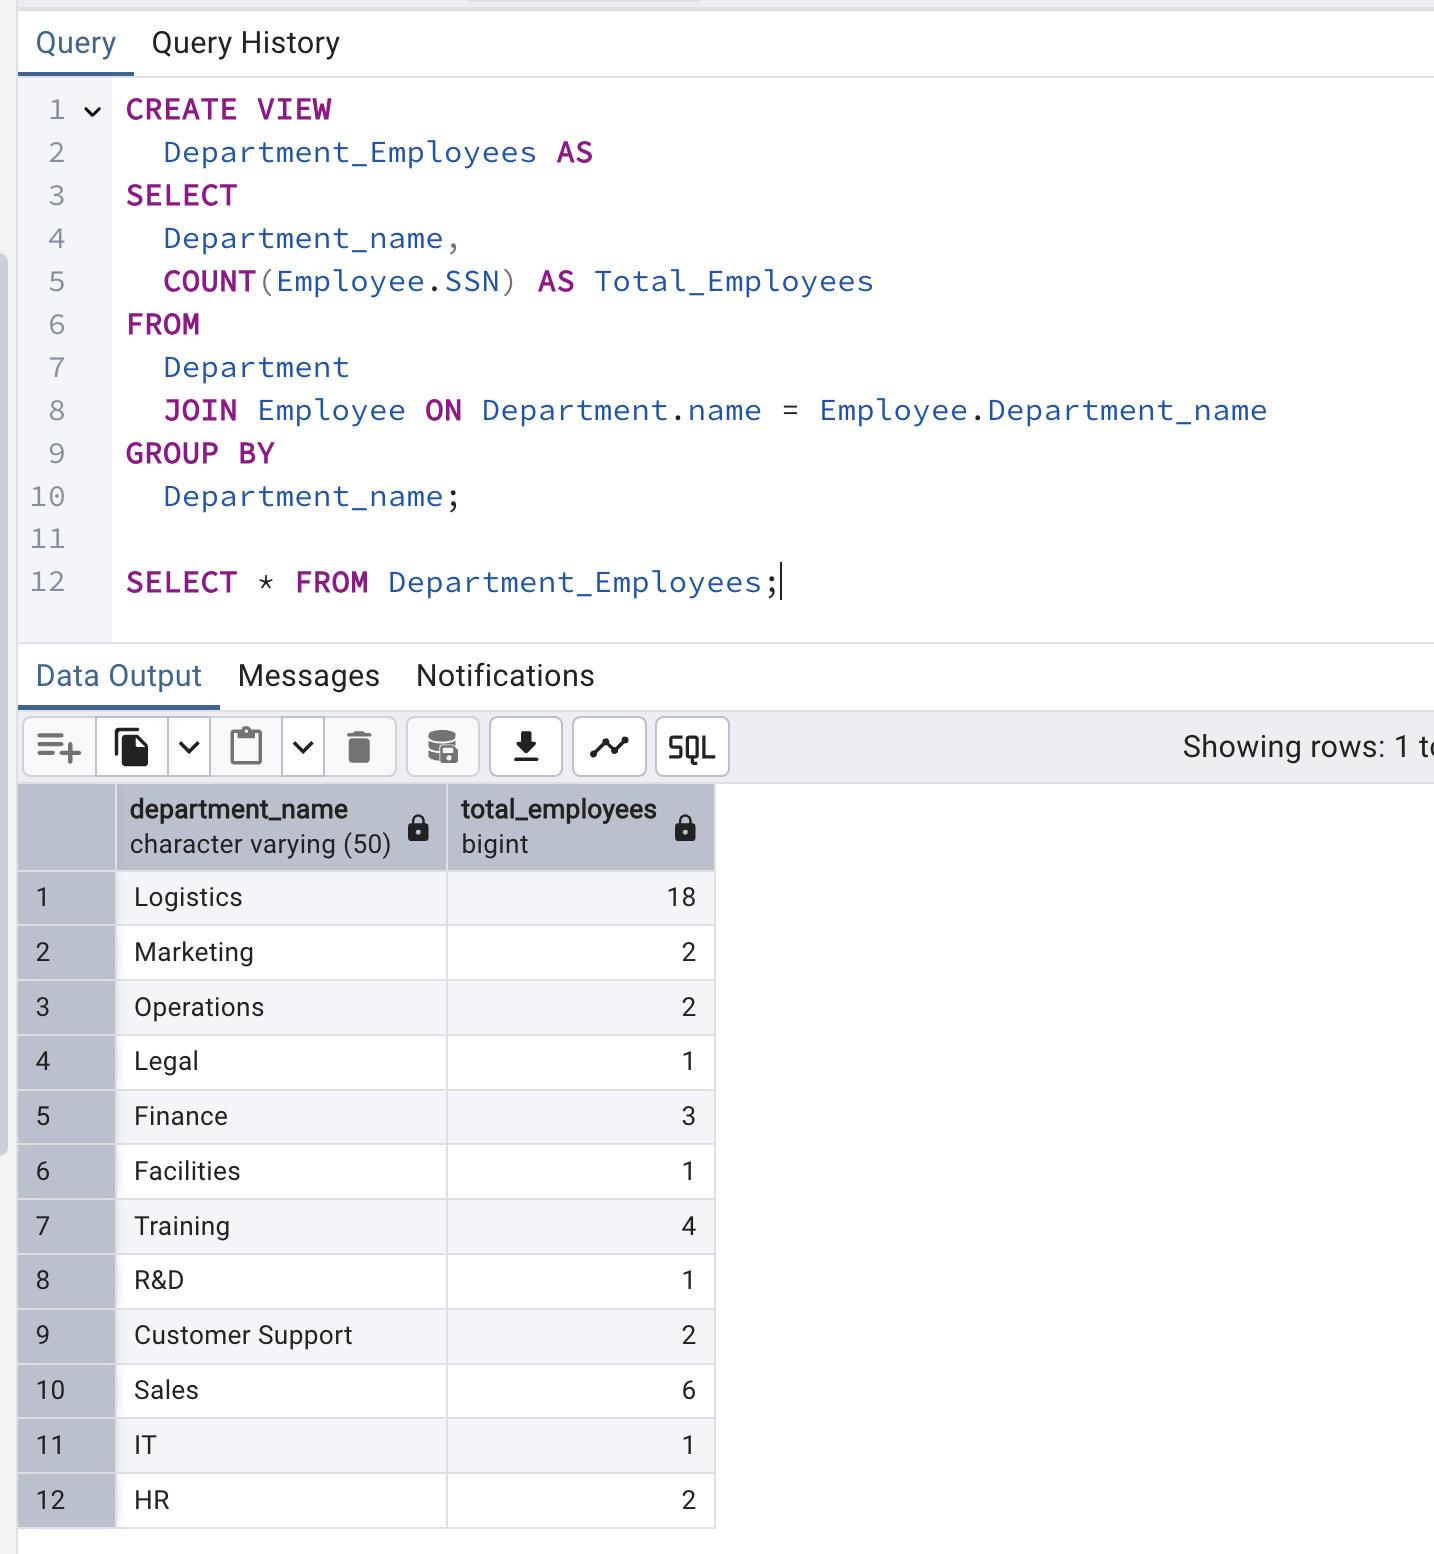
\includegraphics[width=1\textwidth]{images/sql/views/update_number_of_employees_in_department.png}
  \caption{\textit{Update of the Number of Employees in the Department View}}
\end{figure}

The Department\_Employees view is necessary for our DBMS as it provides a simplified and aggregated representation of the number of employees in each department. By creating this view, we can easily query and retrieve the total count of employees per department without repeatedly writing complex SQL joins and group by operations. This enhances query efficiency, improves readability, and ensures consistency in how this specific data is accessed and reported across different parts of the application.

\subsubsection{Total Revenue Generated by Each Product}

\lstinputlisting[language=SQL, caption={\textit{Total Revenue Generated by Each Product View}}]{sql/views/total_revenue_generated_by_each_product.sql}

Creating the Product\_Revenue view is necessary to simplify and streamline the process of analyzing the total revenue generated by each product. By encapsulating the SQL query within a view, you provide a reusable and easily accessible way to retrieve this aggregated data without repeatedly writing the same complex query. This enhances code maintainability, improves readability, and ensures consistency in how revenue data is calculated and presented across different parts of the application or for various reporting purposes

\subsection{Triggers}

\subsubsection{Update Product Revenue Trigger}

\lstinputlisting[language=SQL, caption={\textit{Update Product Revenue Trigger}}]{sql/triggers/update_product_revenue.sql}

This code defines a PostgreSQL trigger and its associated function to automatically update the total revenue for a product whenever a new order is placed. The Update\_Product\_Revenue function increments the Total\_Revenue in the Product\_Revenue table by the amount of the newly inserted order (NEW.Amount) for the corresponding product (NEW.Product\_SKU). This trigger is set to fire after an insert operation on the Purchased table, ensuring that the revenue data remains accurate and up-to-date without manual intervention. This trigger is important because it maintains data integrity and consistency by automating the update process, reducing the risk of human error and ensuring that revenue calculations are always current.

\subsubsection{Update Customer Orders Trigger}

\lstinputlisting[language=SQL, caption={\textit{Update Customer Orders Trigger}}]{sql/triggers/update_customer_orders.sql}

This code defines a PostgreSQL trigger and a corresponding function to automatically update the total number of orders placed by each customer whenever a new order is inserted into the Order table. The Update\_Customer\_Orders function increments the Total\_Orders field in the Customer\_Orders table for the customer associated with the new order, identified by their phone number. The trigger Update\_Customer\_Orders is set to execute this function after each new row is inserted into the Order table. This automation ensures that the Total\_Orders count remains accurate and up-to-date without requiring manual updates, thereby maintaining data integrity and consistency.

\subsubsection{Update Department Employees Trigger}

\lstinputlisting[language=SQL, caption={\textit{Update Department Employees Trigger}}]{sql/triggers/update_department_employees.sql}

This code defines a PostgreSQL trigger function named Update\_Department\_Employees that updates the total number of employees in a department whenever a new employee is added. The function increments the Total\_Employees field in the Department\_Employees table by 1 for the department specified in the NEW.Department\_name field, which represents the department of the newly added employee. This trigger is important because it ensures that the Total\_Employees count in the Department\_Employees table is always accurate and up-to-date, reflecting the current number of employees in each department without requiring manual updates or additional queries. This helps maintain data integrity and consistency within the database.

\subsubsection{Update Department Employees Remove Trigger}

\lstinputlisting[language=SQL, caption={\textit{Update Department Employees Remove Trigger}}]{sql/triggers/update_department_employees_remove.sql}

This code defines a PostgreSQL trigger and a corresponding function to automatically update the total number of employees in a department whenever an employee is removed from the Employee table. The Update\_Department\_Employees\_Remove function decreases the Total\_Employees count in the Department\_Employees table by 1 for the department from which the employee was deleted. The trigger Update\_Department\_Employees\_Remove is set to fire after a delete operation on the Employee table, ensuring the department's employee count remains accurate. This automation is useful for maintaining data integrity and consistency without requiring manual updates.

\subsubsection{Update Product Revenue Sold Trigger}

\lstinputlisting[language=SQL, caption={\textit{Update Product Revenue Sold Trigger}}]{sql/triggers/update_product_revenue_sold.sql}

This code defines a PostgreSQL trigger and a corresponding function to automatically update the total revenue for a product whenever a new sale is recorded. The Update\_Product\_Revenue\_Sold function increments the Total\_Revenue in the Product\_Revenue table by the amount of the newly inserted sale (NEW.Amount) for the product identified by NEW.Product\_SKU. This trigger is set to fire after an insert operation on the Purchased table, ensuring that every time a new purchase record is added, the total revenue for the corresponding product is updated accordingly. This mechanism is necessary to maintain accurate and up-to-date revenue data without requiring manual updates, thereby reducing the risk of errors and improving data consistency.

\subsection{Functions}

\subsubsection{Get Product Revenue Function}

\lstinputlisting[language=SQL, caption={\textit{Get Product Revenue Function}}]{sql/functions/get_product_revenue.sql}

This SQL script defines a function named Get\_Product\_Revenue using PL/pgSQL, a procedural language for PostgreSQL. The function calculates the total revenue generated by a specific product identified by its Product\_SKU. It does this by summing the Amount from the Purchased table where the Product\_SKU matches the input parameter. The result is stored in the Total\_Revenue variable and then returned. This function is necessary because it encapsulates the logic for revenue calculation into a reusable and maintainable unit, allowing for consistent and efficient retrieval of revenue data for any product across the database.

\begin{figure}[H]
  \centering
  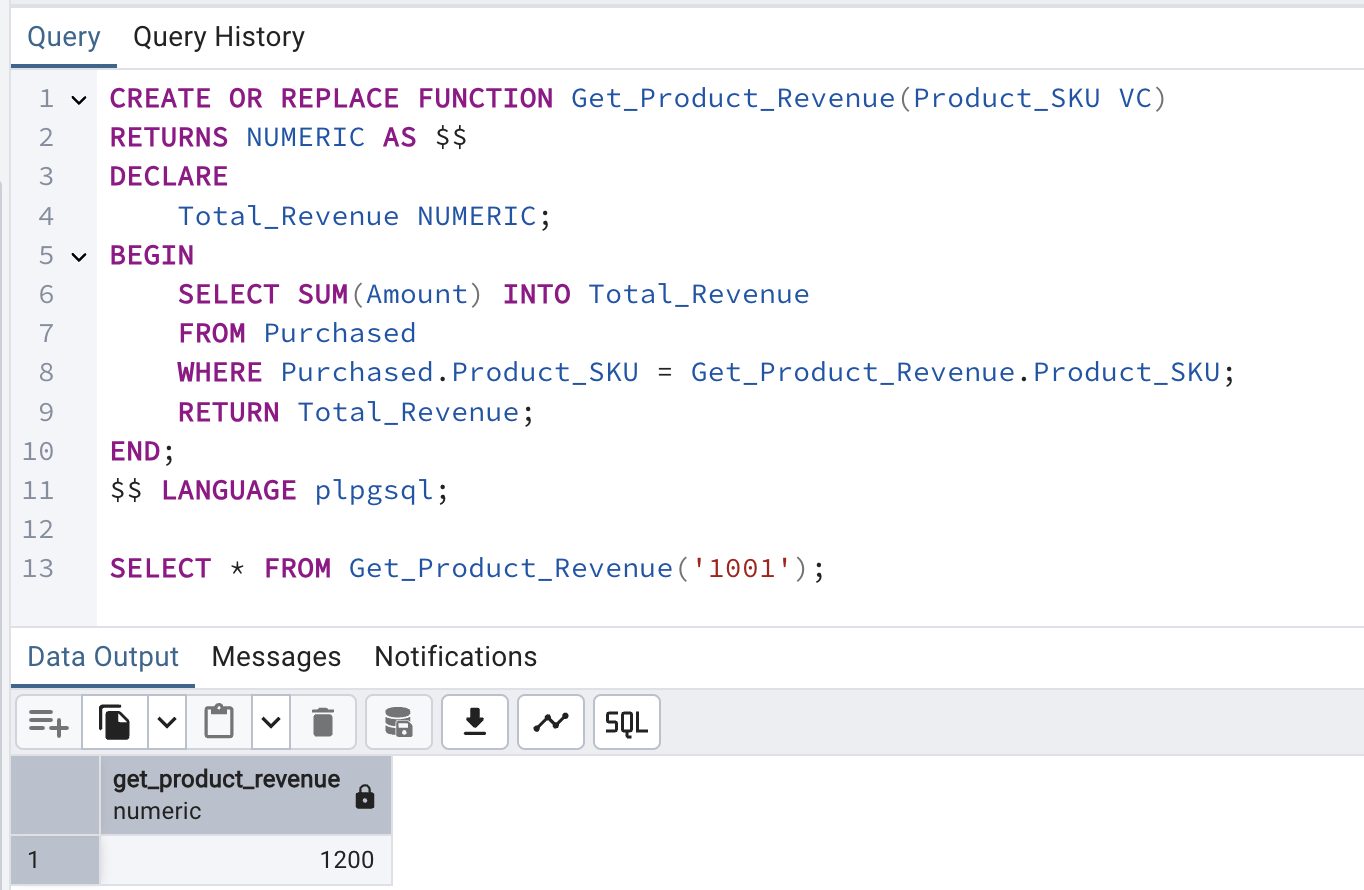
\includegraphics[width=1\textwidth]{images/sql/functions/get_product_revenue.png}
  \caption{\textit{Get Product Revenue Function}}
\end{figure}

\subsubsection{Get Customer Orders Function}

\lstinputlisting[language=SQL, caption={\textit{Get Customer Orders Function}}]{sql/functions/get_customer_orders.sql}

This SQL code defines a function named Get\_Customer\_Orders that calculates the total number of orders placed by a specific customer, identified by their phone number. The function takes a customer's phone number as an input parameter and returns an integer representing the total count of orders. Inside the function, a variable Total\_Orders is declared to store the result of a SELECT COUNT(Order\_id) query, which counts the number of orders associated with the given phone number in the Order table. This function is useful for quickly retrieving the number of orders for a customer, which can be helpful for customer relationship management, analytics, and reporting purposes. Note that the function uses PL/pgSQL, a procedural language for PostgreSQL.

\begin{figure}[H]
  \centering
  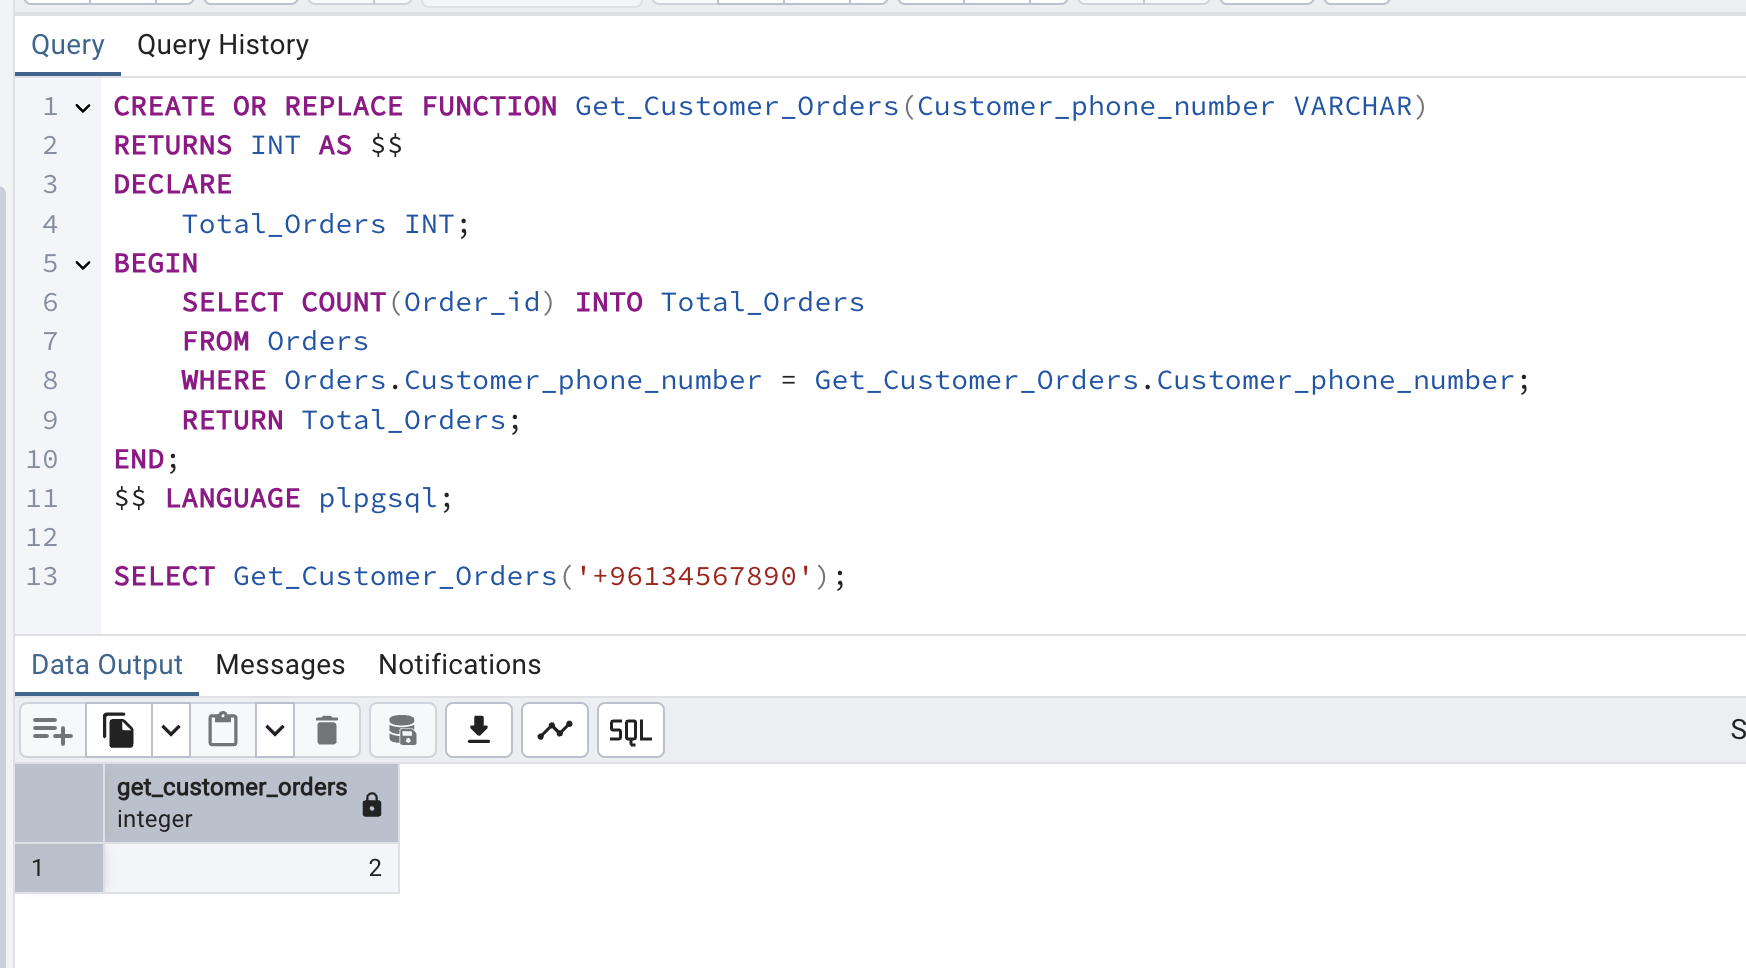
\includegraphics[width=1\textwidth]{images/sql/functions/get_customer_orders.png}
  \caption{\textit{Get Customer Orders Function}}
\end{figure}

\subsubsection{Get Department Employees Function}

\lstinputlisting[language=SQL, caption={\textit{Get Department Employees Function}}]{sql/functions/get_department_employees.sql}

This SQL script defines a function named Get\_Department\_Employees that calculates the total number of employees in a specific department. The function takes a single parameter, Department\_name, which is the name of the department for which the employee count is needed. Inside the function, a variable Total\_Employees is declared to store the count of employees. The SELECT COUNT(SSN) INTO Total\_Employees statement counts the number of employees (identified by their SSN) in the specified department and stores the result in Total\_Employees. Finally, the function returns this count. This function is useful for quickly retrieving the number of employees in any given department, which can be helpful for reporting and analysis purposes in a database management system.

\begin{figure}[H]
  \centering
  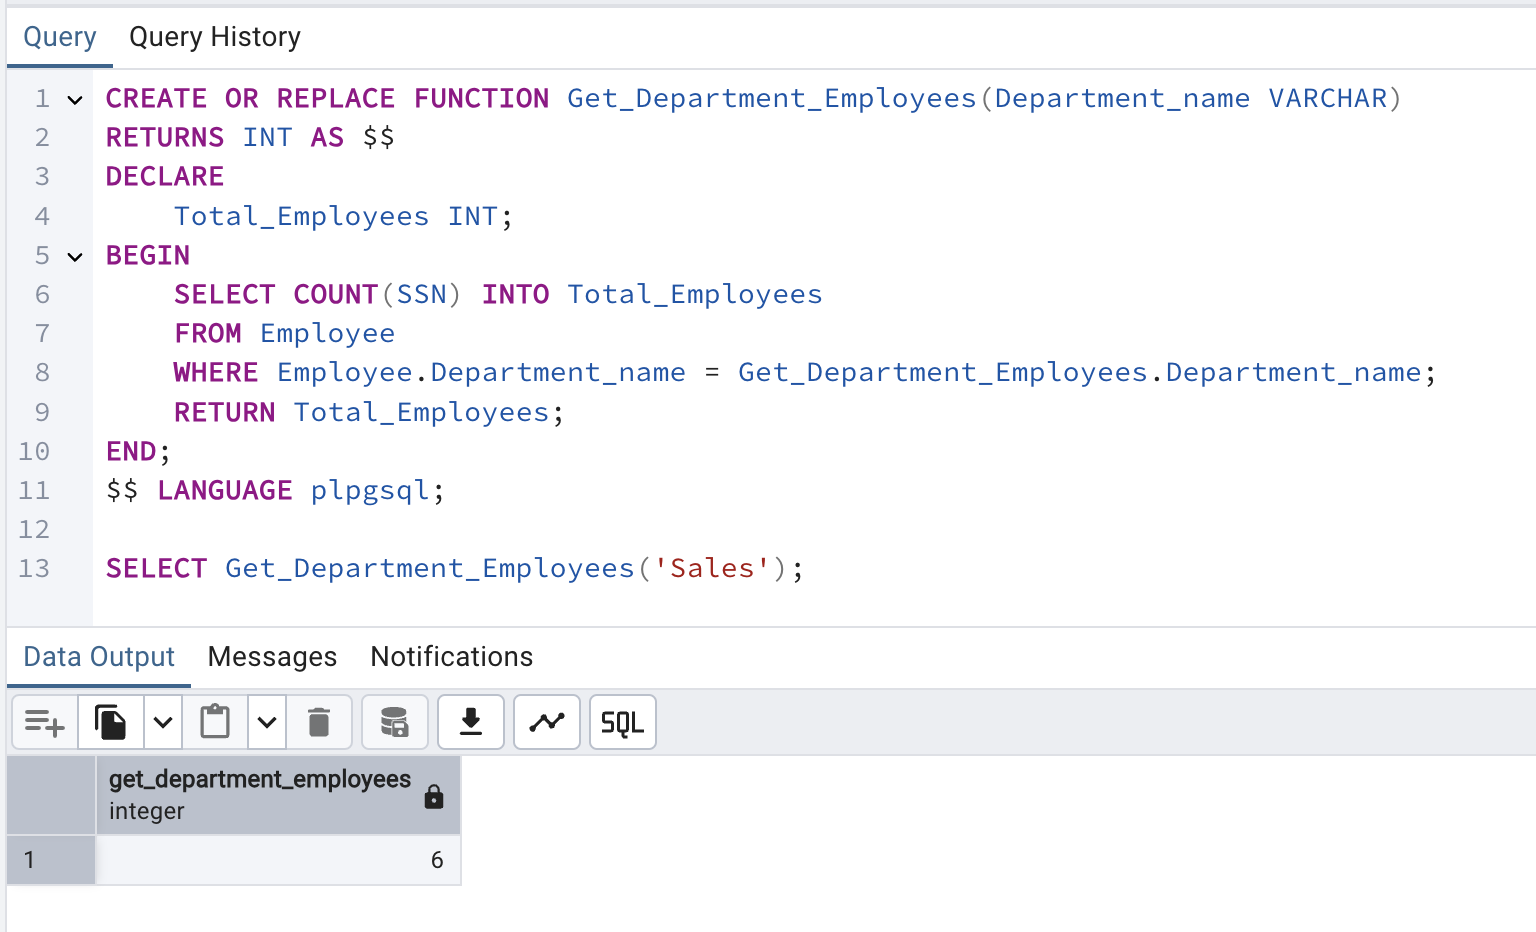
\includegraphics[width=1\textwidth]{images/sql/functions/get_department_employees.png}
  \caption{\textit{Get Department Employees Function}}
\end{figure}

\subsection{Stored Procedures}

\subsubsection{Calculate Category Revenue Procedure}

\lstinputlisting[language=SQL, caption={\textit{Calculate Category Revenue Procedure}}]{sql/stored-procedures/calculate_category_revenue.sql}

This SQL script creates a stored procedure named Calculate\_Category\_Revenue in PL/pgSQL, which is a procedural language for PostgreSQL. The procedure takes a single parameter, Category\_name, which specifies the product category for which the total revenue needs to be calculated. Inside the procedure, a variable Total\_Revenue is declared to store the sum of the amounts from the Purchased table. The procedure performs a SELECT query that joins the Purchased table with the Product table on the Product\_SKU field and filters the results by the given Category\_name. The total revenue is then stored in the Total\_Revenue variable. Finally, the procedure raises a notice displaying the total revenue for the specified category. This query is useful for businesses to quickly calculate and report the total revenue generated by different product categories, aiding in financial analysis and decision-making.

\begin{figure}[H]
  \centering
  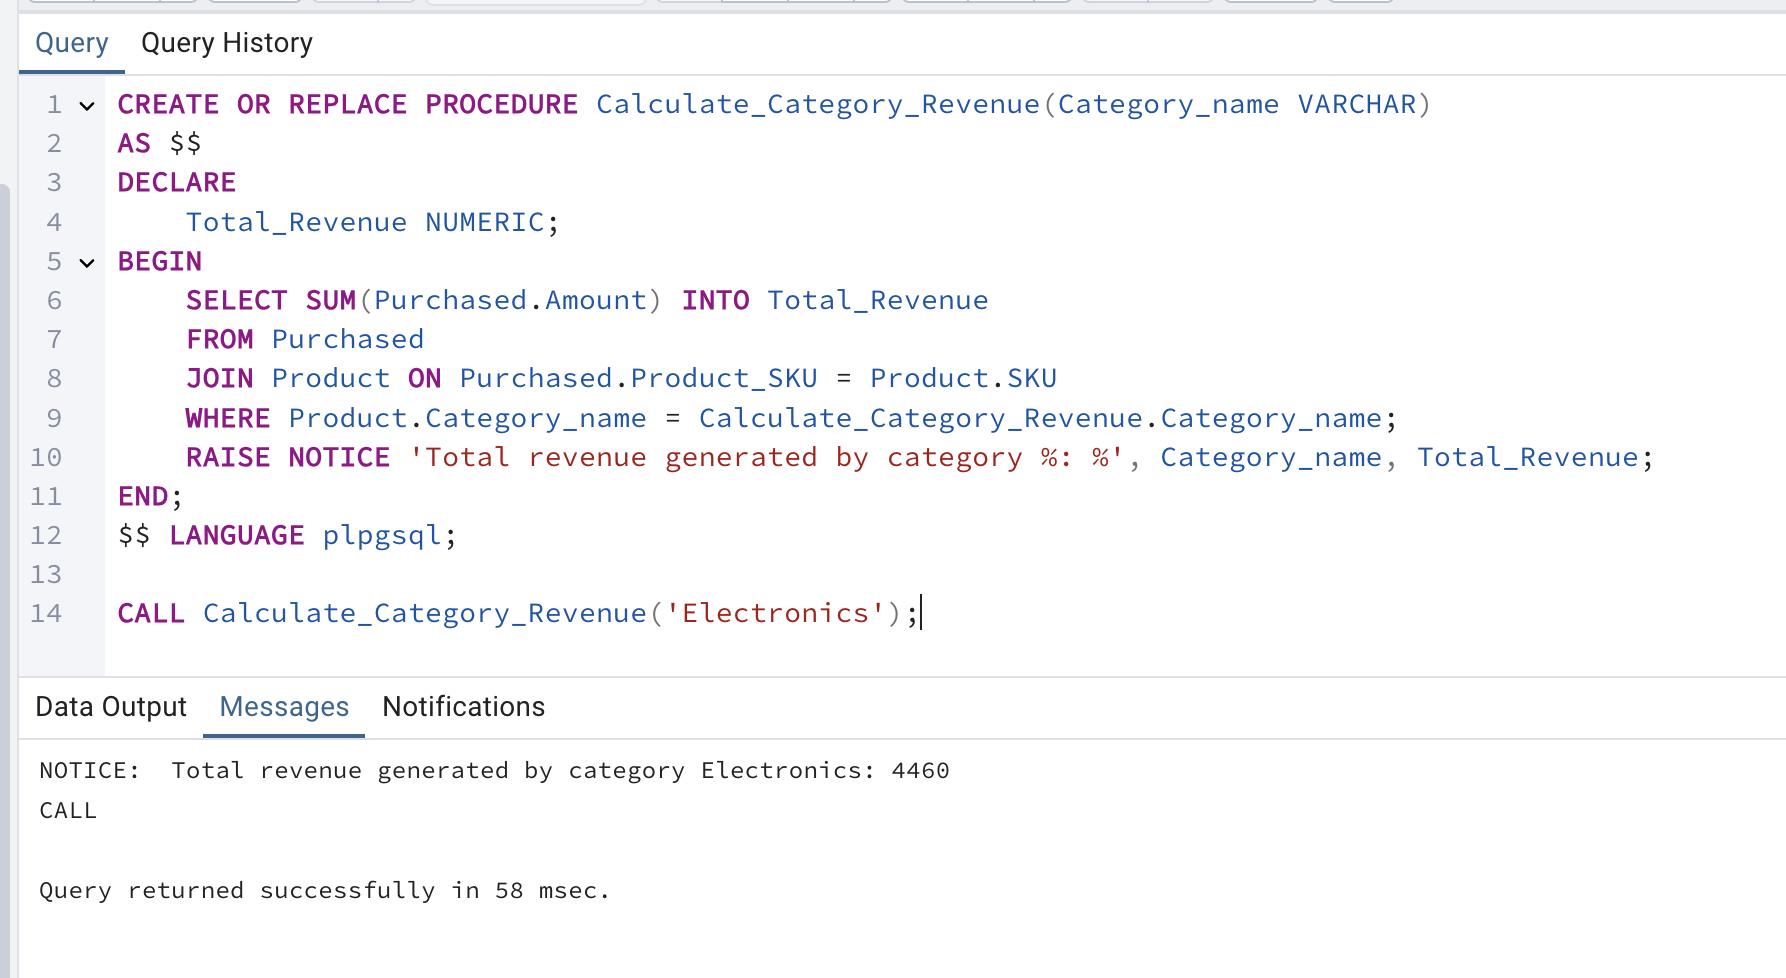
\includegraphics[width=1\textwidth]{images/sql/stored-procedures/calculate_category_revenue.png}
  \caption{\textit{Calculate Category Revenue Procedure}}
\end{figure}
